\documentclass[10pt, landscape]{article}
\usepackage[scaled=0.92]{helvet}
\usepackage{multicol}
\usepackage{calc}
\usepackage{ifthen}
\usepackage[landscape]{geometry}
%\usepackage{hyperref}

\usepackage{newtxtext} 

%for strikeout
\usepackage{ulem}

%For editing parbox
\usepackage[table]{xcolor}
%For editing itemise margins, reduce iterm separaion and list separation
\usepackage{enumitem}
% For math
\usepackage{amsmath,amsthm,amsfonts,amssymb}

%For pictures / figures
\usepackage{color,graphicx,overpic}
\graphicspath{ {./images/} }

%\usepackage{newtxtext} 
%\usepackage{amssymb}
%\usepackage[table]{xcolor}
%\usepackage{vwcol}
%\usepackage{tikz}
%\usepackage{wrapfig}
%\usepackage{makecell}

\pdfinfo{
  /Title (CS2106-notes.pdf)
  /Creator (Ger Teck)
  /Author (Ger Teck)
  /Subject ()
  /Keywords (tex)}

%% Margins for PAPER

% This sets page margins to .5 inch if using letter paper, and to 1cm
% if using A4 paper. (This probably isn't strictly necessary.)
% If using another size paper, use default 1cm margins.
\ifthenelse{\lengthtest { \paperwidth = 11in}}
	{ \geometry{top=.3in,left=.3in,right=.3in,bottom=.3in} }
	{\ifthenelse{ \lengthtest{ \paperwidth = 297mm}}
		{\geometry{top=0.5cm,left=0.5cm,right=0.5cm,bottom=0.5cm} }
		{\geometry{top=0.5cm,left=0.5cm,right=0.5cm,bottom=0.5cm} }
	}

% Turn off header and footer
\pagestyle{empty}
% for tight centres (less spacing)
\newenvironment{tightcenter}{%
  \setlength\topsep{0.5pt}
  \setlength\parskip{0.5pt}
  \begin{center}
}{%
  \end{center}
}

% Redefine section commands to use less space
\makeatletter
\renewcommand{\section}{\@startsection{section}{1}{0mm}%
                                {-1ex plus -.5ex minus -.2ex}%
                                {0.5ex plus .2ex}%x
                                {\normalfont\large\bfseries}}
\renewcommand{\subsection}{\@startsection{subsection}{2}{0mm}%
                                {-1explus -.5ex minus -.2ex}%
                                {0.5ex plus .2ex}%
                                {\normalfont\normalsize\bfseries}}
\renewcommand{\subsubsection}{\@startsection{subsubsection}{3}{0mm}%
                                {-1ex plus -.5ex minus -.2ex}%
                                {1ex plus .2ex}%
                                {\normalfont\small\bfseries}}
% change font
%\renewcommand{\familydefault}{\sfdefault}
%\renewcommand\rmdefault{\sfdefault}
\linespread{1.05}

\makeatother

% Define BibTeX command
\def\BibTeX{{\rm B\kern-.05em{\sc i\kern-.025em b}\kern-.08em
    T\kern-.1667em\lower.7ex\hbox{E}\kern-.125emX}}

% Don't print section numbers
\setcounter{secnumdepth}{0}

\setlength{\parindent}{0pt}
\setlength{\parskip}{0pt plus 0.5ex}

%% this changes all items (enumerate and itemize, reduce margins) ITEMIZE SEPARATION HERE
\setlength{\leftmargini}{0.5cm}
\setlength{\leftmarginii}{0.5cm}
\setlist[itemize,1]{leftmargin=2mm,labelindent=1mm,labelsep=1mm, itemsep = 0mm}
\setlist[itemize,2]{leftmargin=4mm,labelindent=1mm,labelsep=1mm, itemsep = 0mm}

% For Code Blocks
\usepackage{xcolor}
\usepackage{listings}

\lstdefinestyle{mystyle}{
	backgroundcolor=\color{gray!25!white},
	basicstyle=\scriptsize,
	numbers=none,    %or = none or left
	showstringspaces=false,
	breaklines=true,
	breakatwhitespace=false,                  
	captionpos=b,                    
	keepspaces=true,                                 
	numbersep=5pt,                  
	showspaces=false,                
	showtabs=false,                  
	tabsize=2,
 }
%Helpful:
%[linewidth = 1.0 \linewidth]
%\lstinline{}
% use \code{} for \lstinline with colorbox.
\newcommand{\code}[1]{\colorbox{gray!25!}{\lstinline|#1|}}
\lstset{style=mystyle}

%\begin{lstlisting} [linewidth = 1.0 \linewidth],
% code here
%\end{lstlisting}

%itemsep = 0mm
%\setlist{nosep}

% -------------------------------------------------------------------------------

% START OF DOCUMENT HERE

\begin{document}
\raggedright
\footnotesize
\begin{multicols*}{3}

% multicol parameters
% These lengths are set only within the two main columns
%\setlength{\columnseprule}{0.25pt}
\setlength{\premulticols}{1pt}
\setlength{\postmulticols}{1pt}
\setlength{\multicolsep}{1pt}
\setlength{\columnsep}{2pt}

%% DOCUMENT NAME HERE
\begin{center}
     \Large{\textbf{CS2106 Intro Op. Systems Notes}} \\
\end{center}
AY23/24 Sem 2, github.com/gerteck


\section{1. Introduction}
\textbf{Course objectives:} Introduces basic concepts in operating systems. Focusing on: \\
- OS structure and architecture, process management, memory management, file management and OS protection mechanism. \\
- Identify and understand major functionalities of modern operating systems. \\
- Extend and apply the knowledge in future courses.

\textbf{Supplementary Text}: Modern Operating System (5th Edition), by Andrew S. Tanenbaum, Pearson, 2023.

\subsection{Learning Outcomes}
\begin{itemize}
	\item Understand how an \textbf{OS manages computational resources for multiple users and applications, and the impact on application performance}
	\item Appreciate the \textbf{abstractions and interfaces provided by OS}
	\item Write \textbf{multi-process / thread programs} and avoid common pitfalls such as \textbf{deadlocks, starvation and race conditions.}
	\item Write system programs that utilizes \textbf{POSIX} syscall for process, memory and I/O management.
	\item Self-learn and explore advanced OS topics.
	\item Understand important design principles in complex systems.
\end{itemize}

Areas to focus on: Try to understand how things are running in parallel, since we naturally think sequentially. Secondly, how we can manage memory and how they combine and interact (in strange ways), synchronization.

\subsection{Operating System OS}
An OS is a program that acts as an intermediary between a computer user and the computer hardware. Motivation for OS:
\begin{itemize}
\item Manage resources and coordination. (Resource Allocator: Process synchronization, resource sharing)
\item Simplify programming (Abstraction of hardware / hardware virtualization, convenient services)
\item Enforce usage policies
\item Security and protection
\item User Program Portability (across different hardware)
\item Efficiency (Optimize for particular usage and hardware).
\end{itemize}

\textbf{Kernel Mode}: Complete access to all hardware resources. \\
\textbf{User Mode}: Limited / Controlled access to hardware resources.

\hspace{0.5cm}

\centerline{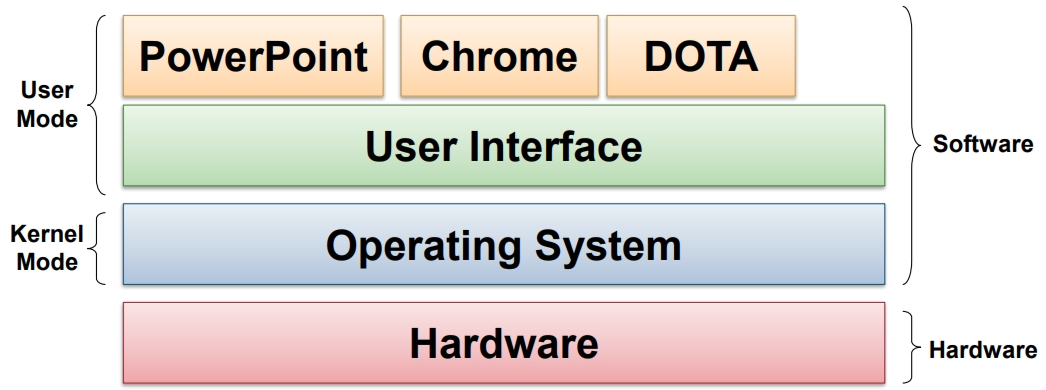
\includegraphics[width=0.5\linewidth]{highlevelOS}}

\subsubsection{Generic OS Components}
\centerline{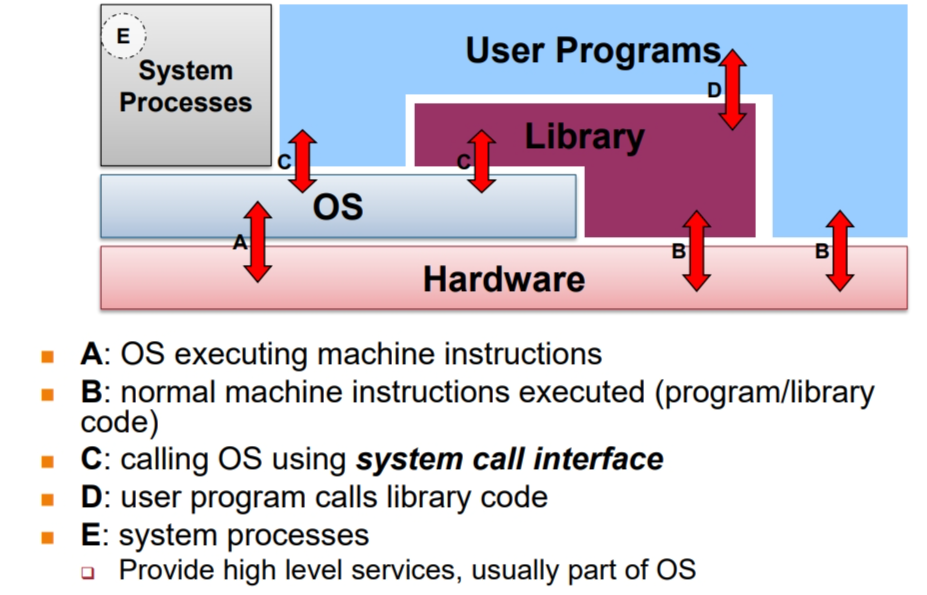
\includegraphics[width=0.7\linewidth]{genericOS}}
\begin{itemize}
\item OS is known as the \textbf{kernel}. \\
		Program that deals with hardware issues, provide system call interface and special code for interrupt handlers, device drivers.
\item Kernel code is different from normal programs: \\
		No use of system call in kernel code, can't use normal libraries, no normal I/O (must do I/O itself).
\item \textbf{Implementing OS}: Historically in assembly/machine, now in HLLs (C, C++). Heavily hardware architecture dependent. Challenges include complexity, debugging, codebase size.
\end{itemize}

\subsubsection{OS Structures}
\textbf{Monolithic OS}: One Big program.
\begin{itemize}
\item Well understood, good performance, but highly coupled components (everything running in kernel mode) and usually devolved into very complicated internal structure.
\end{itemize}

\textbf{Microkernel OS}: 
\begin{itemize}
\item Kernel is very small and clean, only providing basic and essential facilities.
\item Inter-Process Communication \textbf{(IPC)}, Address space management, Thread management etc.
\item Higher level services are built on top of basic facilities, run as server process \textit{outside} of OS, use IPC to communicate.
\item Kernel is more robust and extendible, better isolation and protection between kernel and high level services. But, lower performance. (Latency)
\end{itemize}
\centerline{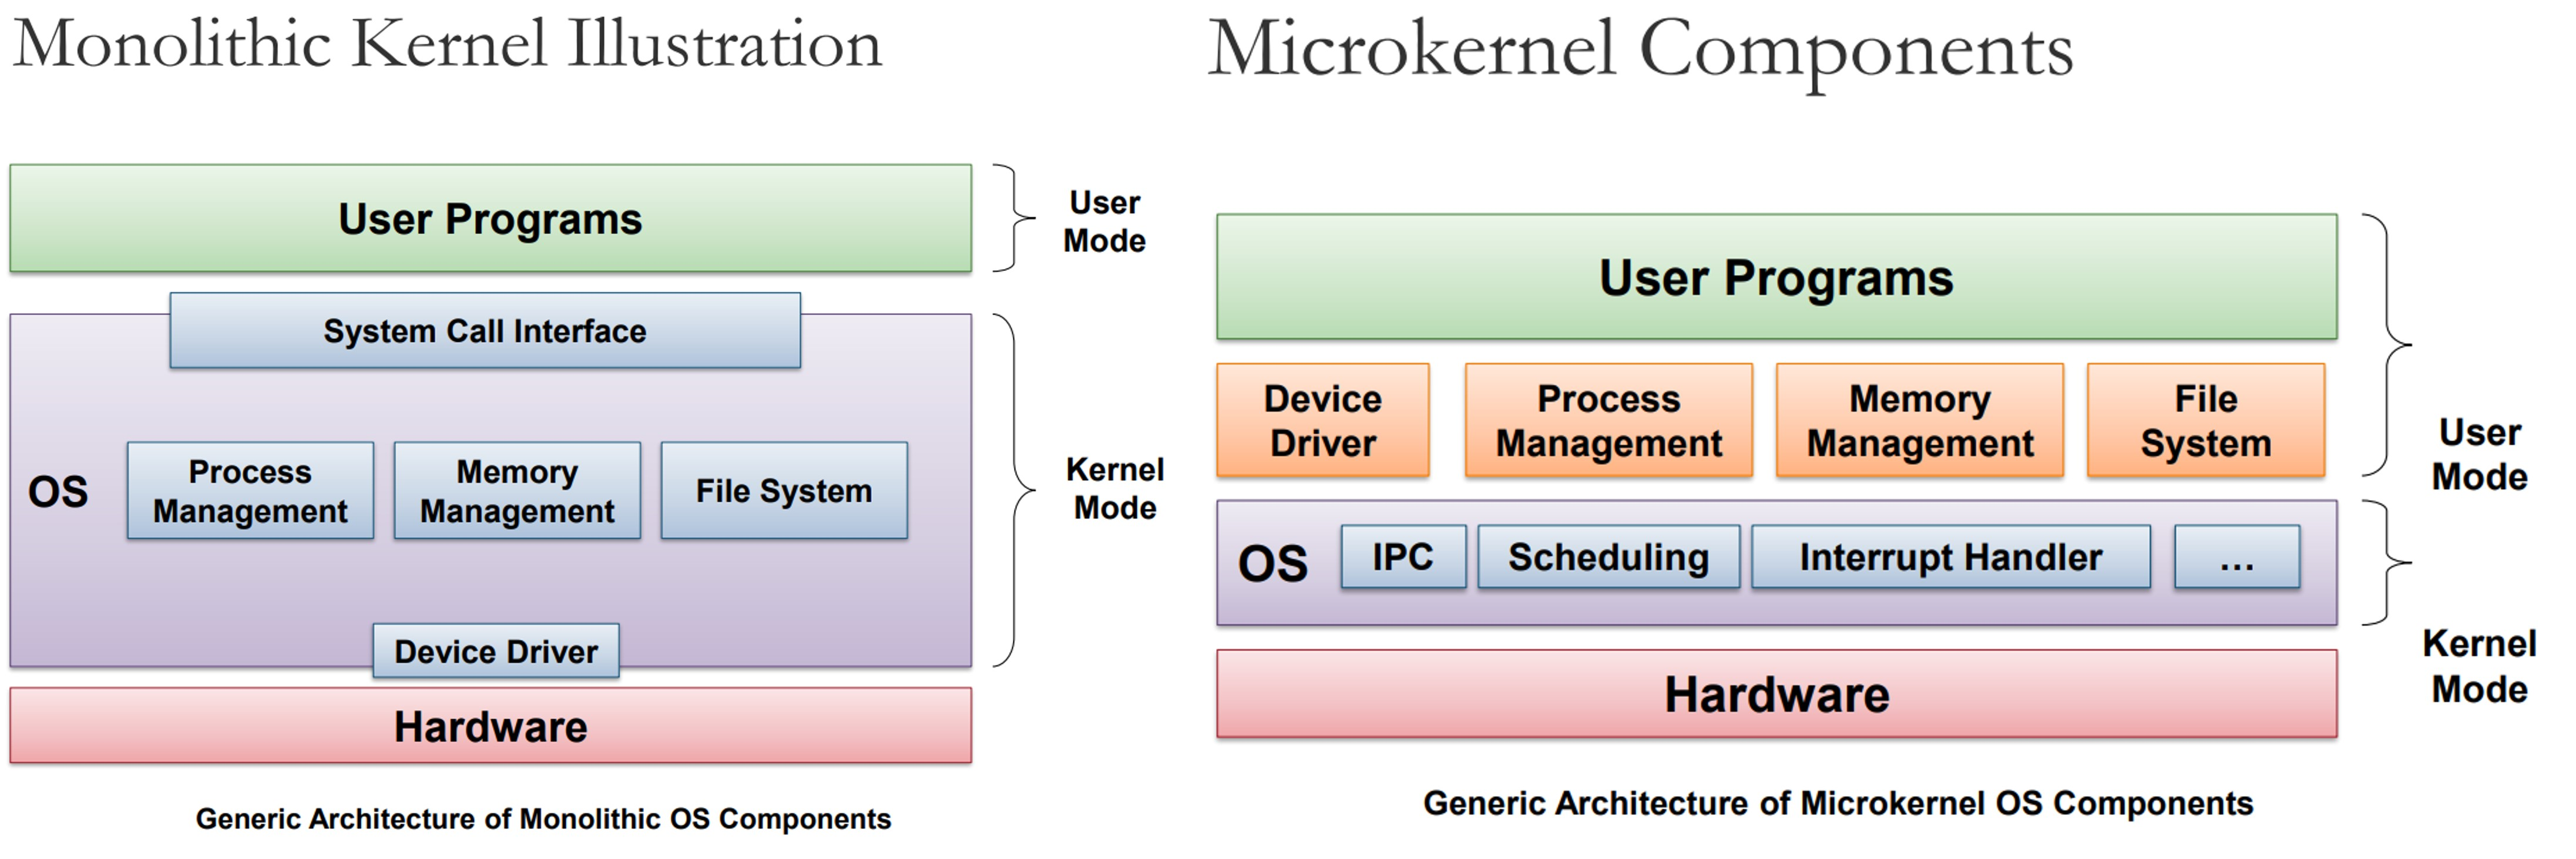
\includegraphics[width=0.95\linewidth]{OSstructure}}

\textbf{Other OS Structure}
\begin{itemize}
\item \textbf{Layered Systems}: Generalization of monolithic system, organize components into hierarchy of layers. Lowest is hardware, highest is user interface.
\item \textbf{Client-Server Model}: Variation of microkernel. Two classes of processes: Client p. request service from server process, server process built on top of microkernel. Client \& Server process can be on separate machine.
\end{itemize}

\subsubsection{Virtual Machines}
\begin{itemize}
\item \textbf{Motivation}: OS assumes total control of hardware, making it hard to run several OS on same hardware at same time. OS is also hard to debug / monitor, hard to observe working of OS, test potentially destructive implementation.
\item \textbf{Virtual Machine}: Software emulation of hardware. 
\item \textbf{Virtualization of underlying hardware}: Illusion of complete hardware to level above. (Memory, CPU etc.) Normal OS can then run on top of virtual machine. Aka \textbf{Hypervisor}. 
	\begin{itemize}
	\item \textbf{Type 1 Hypervisor}: Provides individual virtual machines to guest OSes (e.g. IBM VM/370)
	\item \textbf{Type 2 Hypervisor}: Runs in host OS, Guest OS runs inside Virtual Machine, (e.g. VMware)
	\end{itemize}
\end{itemize}
\centerline{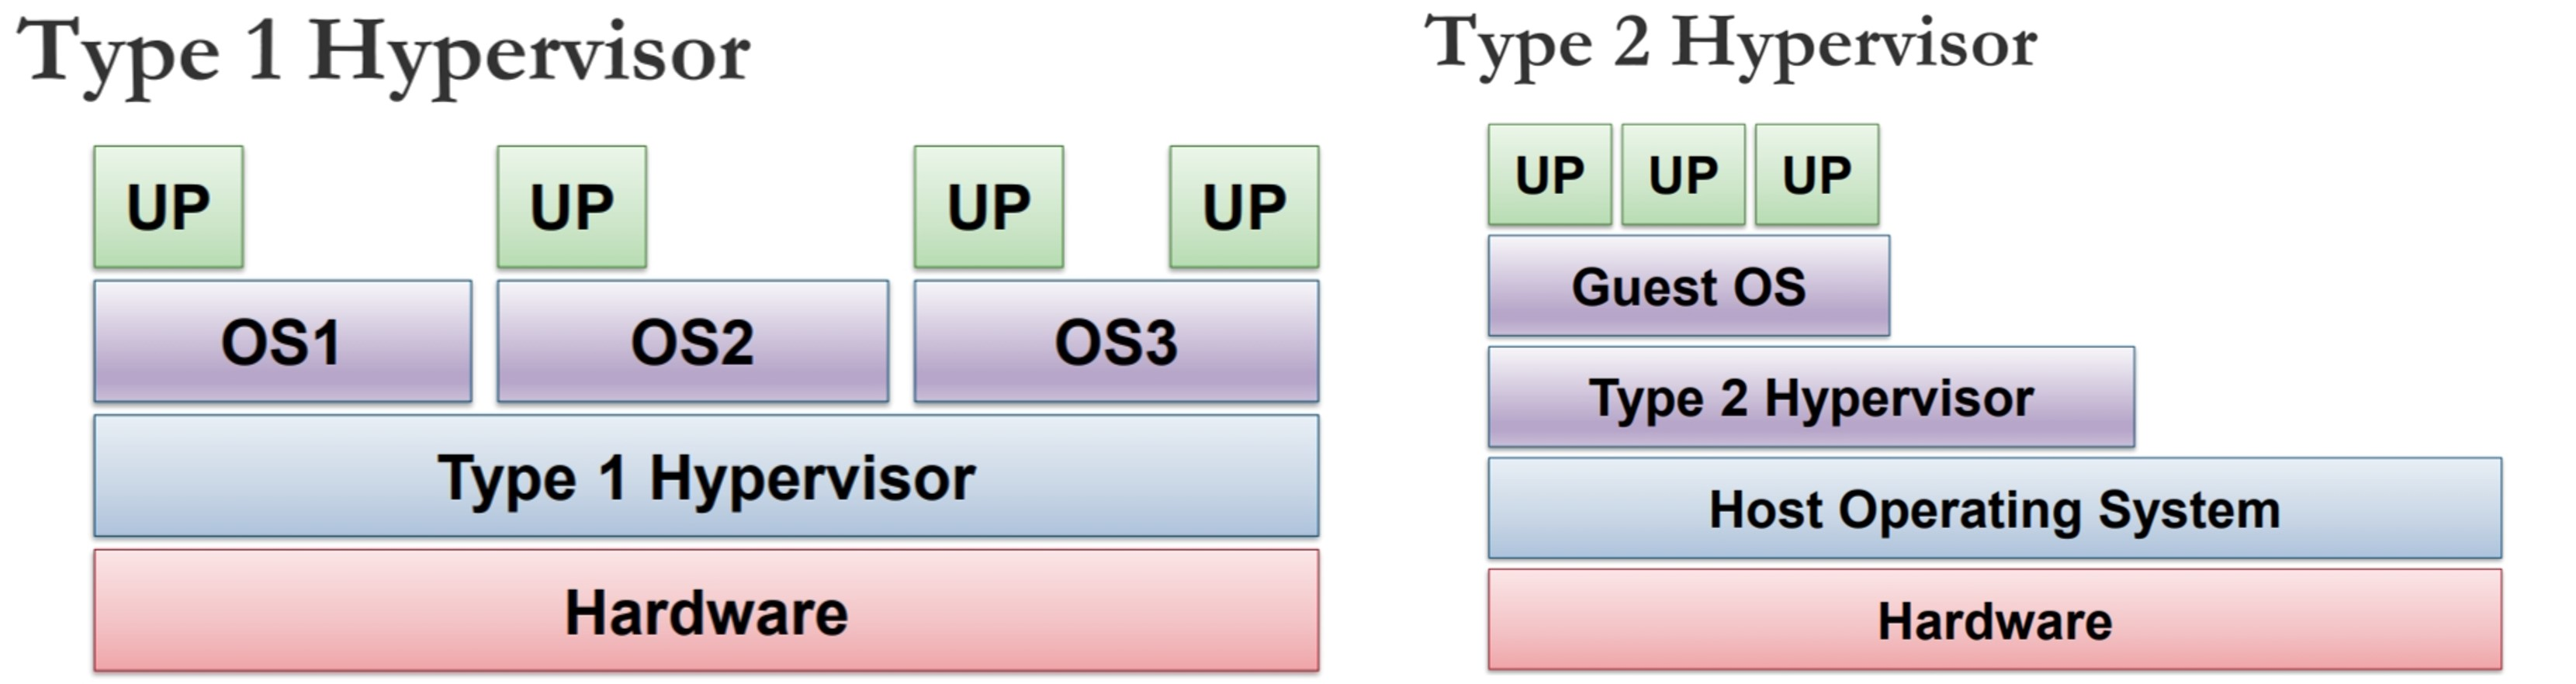
\includegraphics[width=0.9\linewidth]{hypervisor}}

\section{- Upcoming Topics -}
\textbf{OS Process Management}: As OS (to maximise efficiency hardware resources), to be able to switch from running one program to the other (share hardware, e.g. CPU), requires information regarding execution of A stored, and A's information replaced with B's information to run. (E.g. the registers in CPU replaced)
\begin{itemize}
	\item \textbf{2. Process Abstraction}: Info describing executing program
	\item \textbf{3. Process Scheduling}: Deciding which process gets to execute
	\item \textbf{4. Inter-Process Communication}: Passing information between processes (tough)
	\item \textbf{5. Threads + Synchronization}: Alternative to Process (Light-weight process aka Thread)
	\item \textbf{6. Memory Management}
	\item \textbf{7. Disjoint Memory Management}
	\item \textbf{8. File System Management}
	\item \textbf{9. File System Implementation}
\end{itemize}


\null \null \null \null
\null \null \null \null

\columnbreak


\section{2. Process Abstraction}
To switch programs, requires information of both programs. Hence, we need abstraction to describe running program, aka \textbf{process}.
\begin{itemize}
\item \textbf{(Process / Task / Job)} is a dynamic abstraction for executing program. 
\item It is info required to describe a \textit{running program}: \\
- Memory Context (Code/Text, Data, Stack, Heap),\\
- Hardware Context (Register/PC, Stack/Frame Pointer), \\
- OS Context (Process Properties (PID, State), Resources Used).
\end{itemize}

\subsubsection{Computer Organization (Recap)}
\begin{itemize}
\item \textbf{Components}: Memory, Cache, Fetch Unit (Loads instruction, location indicated by special register \textbf{PC}.)
\item \textbf{Functional Units} (Carry out instruction execution, dedicated to diff. instr. type) (CS2100 looked at INT func. unit)
\item Registers (Internal storage, fastest access speed). \\
- \textbf{GPR}: General Purpose Register, accessible by user program / compiler. \\
- \textbf{Special Registers}: PC, Stack/Frame Pointer, PSW etc.
\item \textbf{Binary Executable File}: file in machine language (built by compiler) for specific processor: \\
- Executable (binary) consists two major components: Instr. (Text) \& Data \\
- When under execution, more info: Memory, Hardware, OS context.	
\end{itemize}
\centerline{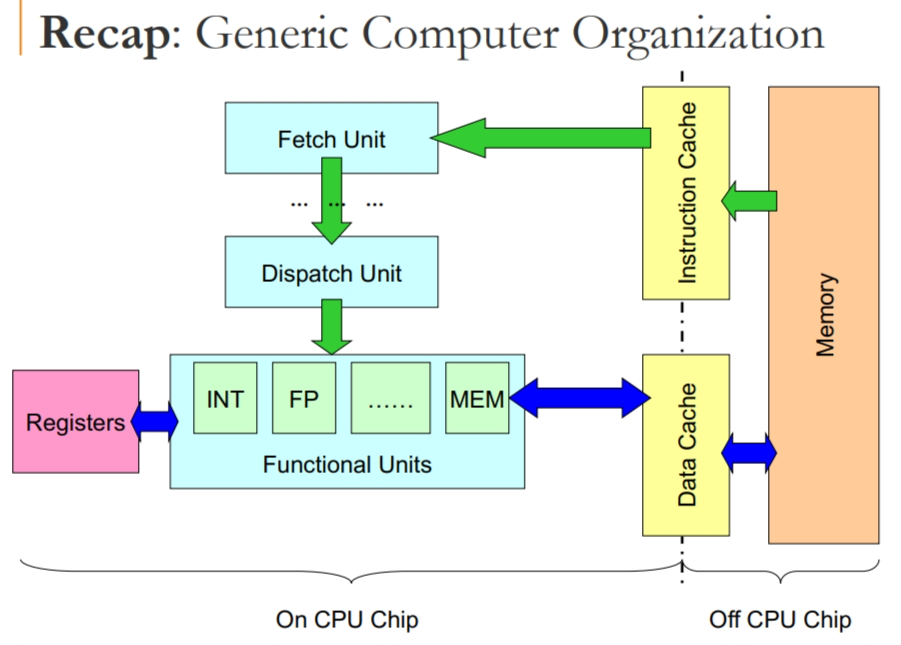
\includegraphics[width=0.6\linewidth]{computerOrg}}

\subsection{Memory Context for Function Call (Stack Memory)}
\textbf{Memory Context Challenges of Functional Calls:}
\begin{itemize}
\item Control Flow Issues: Need to jump to function body, resume after, need to store PC of caller.
\item Data Storage Issues: Need to pass params to function, capture return result, may need declare local variables.
\item Require region of memory dynamically used by function invocations.
\end{itemize}
Hence, portion of memory space used as \textbf{stack memory} that stores executing function using \textbf{stack frame}, which includes usage of \textit{Stack Pointer, Frame Pointer}.

\subsubsection{Stack Memory Region}
\begin{itemize}
\item \textbf{Memory region to store information function invocation.}
\item \textbf{Stack Frame}: Describes information of function invocation.
\item Stack frame added on top when function is invoked, stack "grows", removed from top when function call ends, stack "shrinks".
\item Stack Frame contains return PC address of caller, arguments for function, storage for local variable, etc.
\item \textbf{Stack Pointer}: Indicates top of stack region (first unused memory location). Usually indicated in specialized register.
\end{itemize}


\subsubsection{Function Call Convention: Stack Frame Setup / Teardown}
There are different ways to setup stack frame, known as function call convention, differences about (info stored in frame, which portion of stack frame prepared \& cleared by caller / callee etc). Dependent on hardware \& programming language. \\
\medskip
\textbf{Example Scheme:}
\centerline{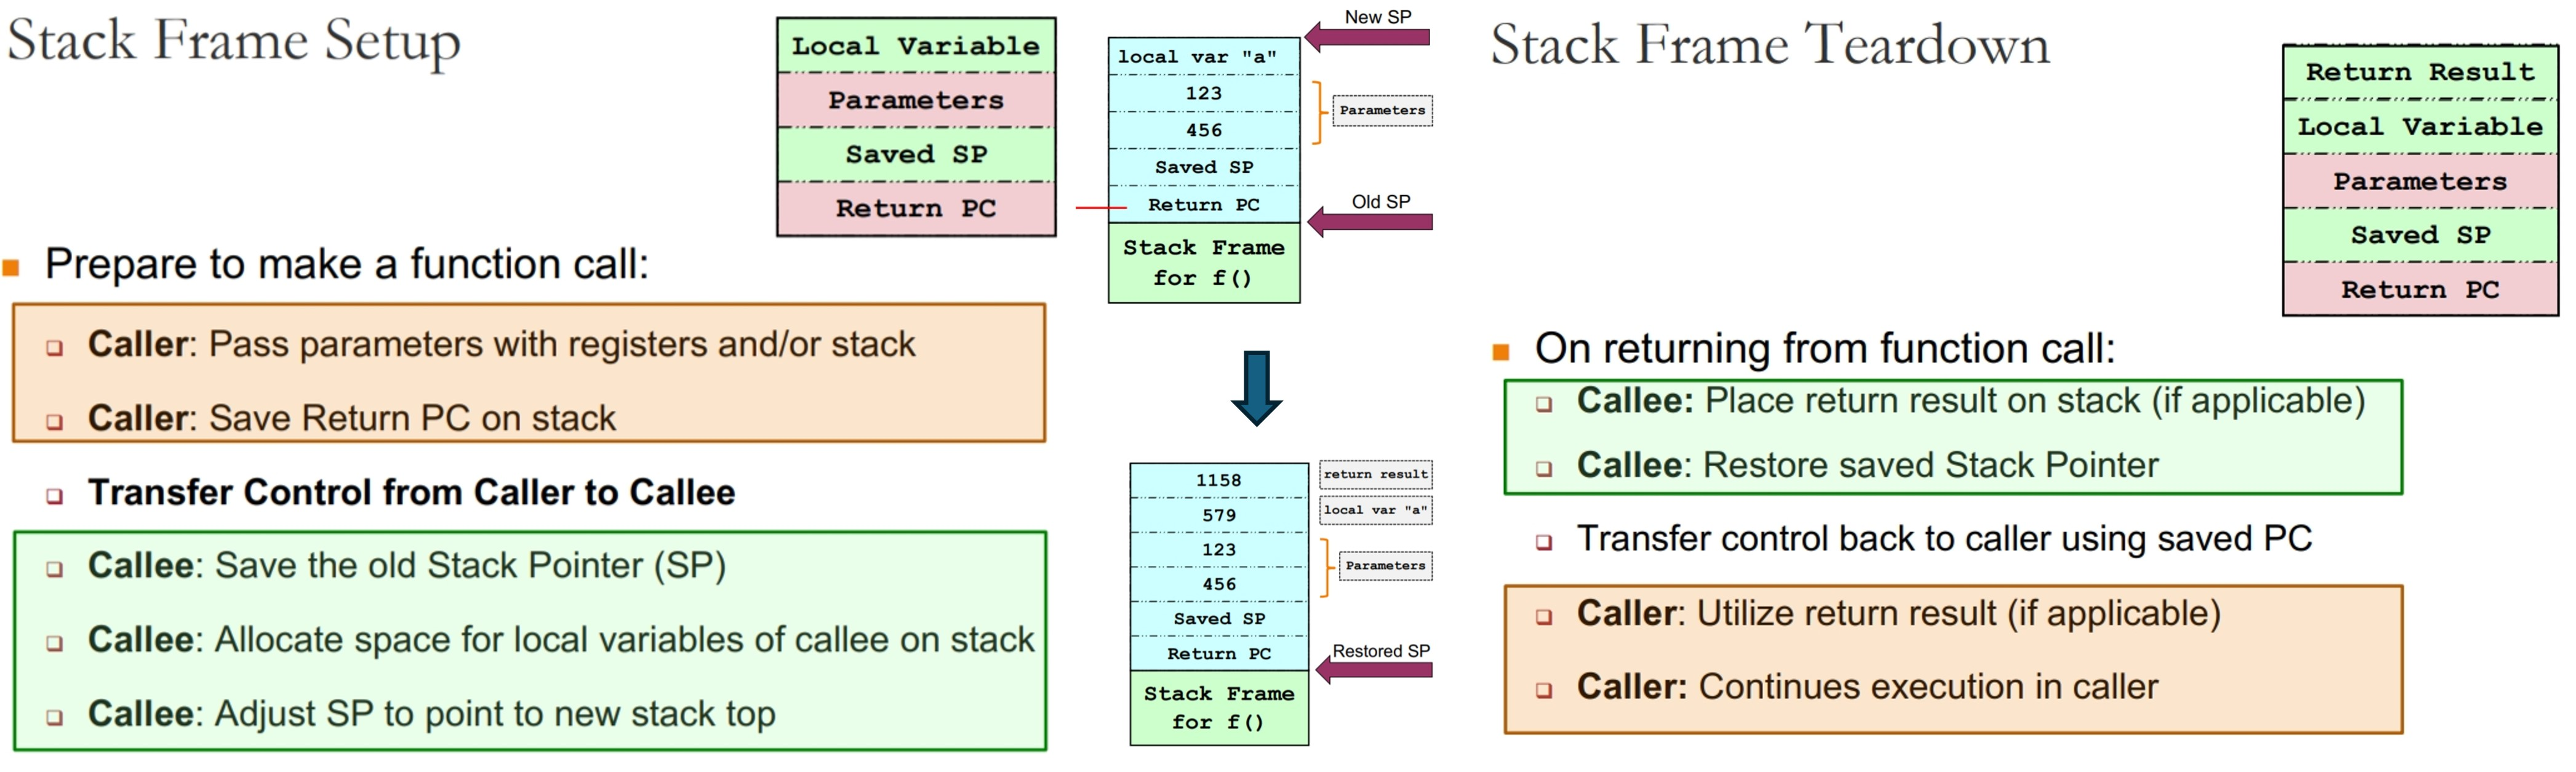
\includegraphics[width=1\linewidth]{stackSetupTeardown}}
\smallskip
\centerline{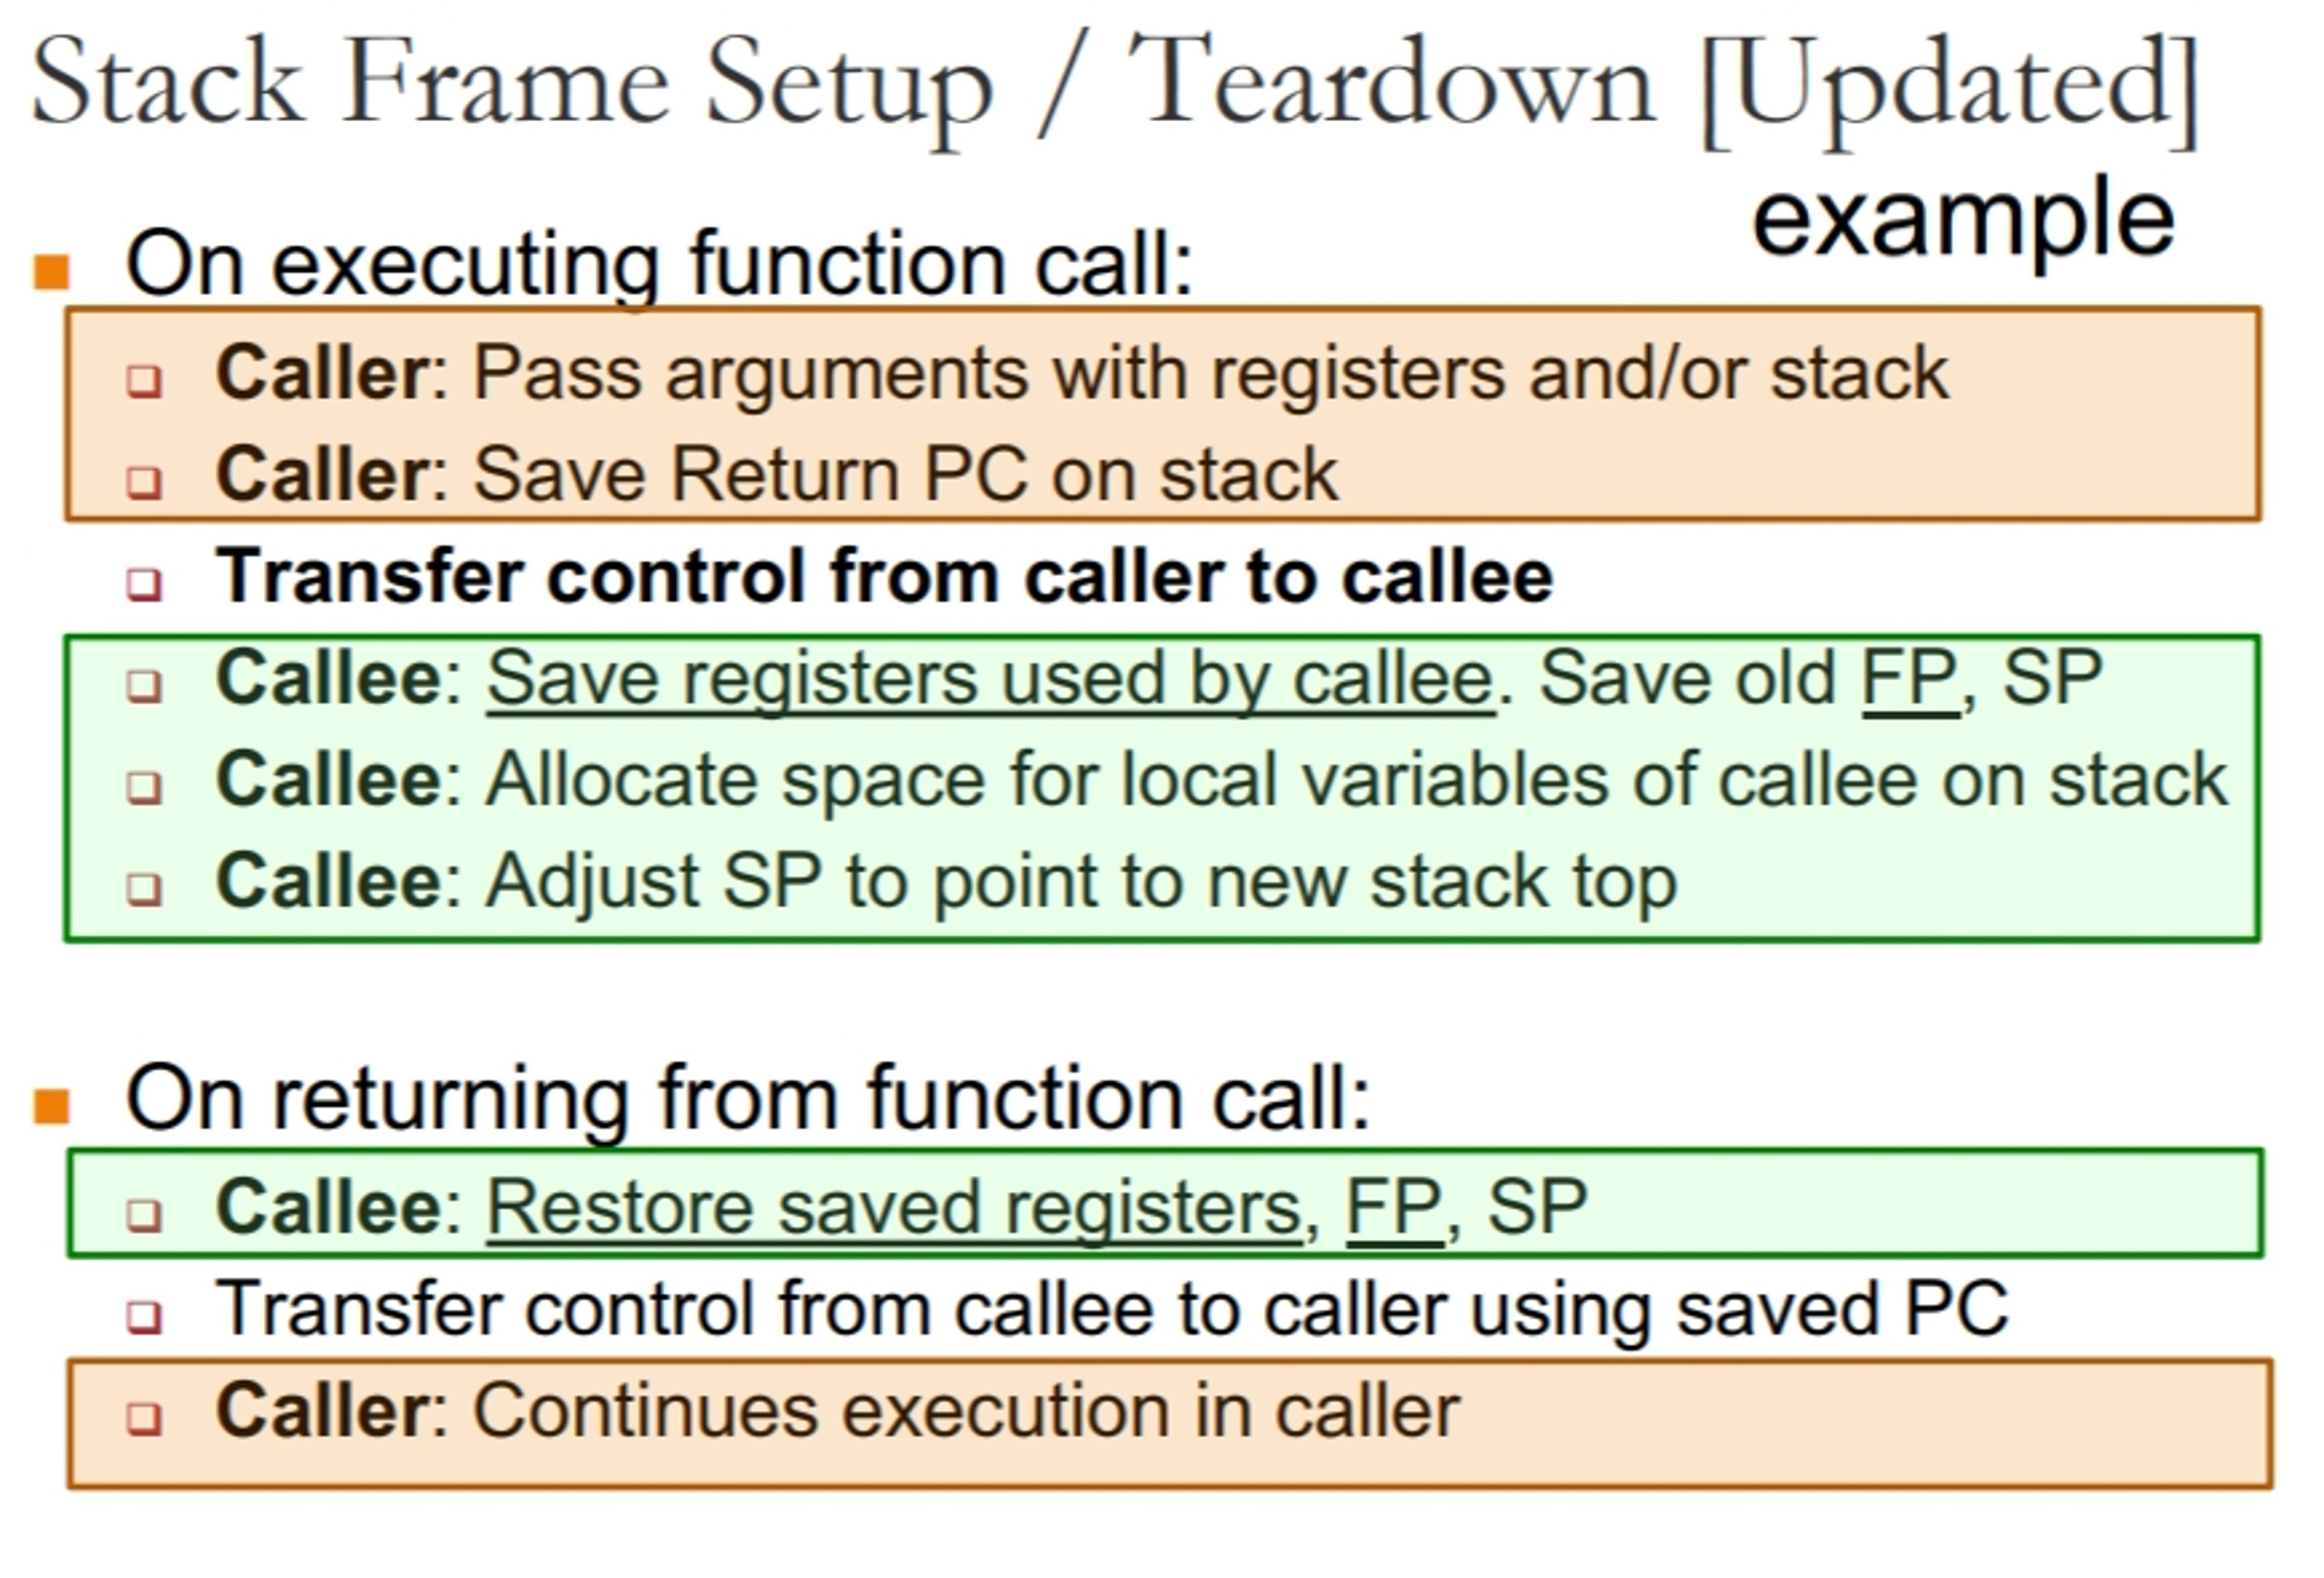
\includegraphics[width=0.45\linewidth]{stackSetupTeardown2}}

\subsubsection{Stack Frame: Other Information}
\textbf{Frame Pointer}
\begin{itemize}
\item To facilitate access of various stack frame items. As stack pointer hard to use as it can change, some processors provide dedicated register Frame Pointer.
\item Frame Pointer points to fixed location in stack frame, other items accessed as displacement from frame pointer, usage of FP is platform dependent.
\end{itemize}

\textbf{Saved Registers}
\begin{itemize}
\item Since number of GPR limited, when GPR exhausted, use memory to temp. hold GPR values for reuse.
\item \textbf{Known as Register Spilling}. Function can spill registers it intends to use before function starts, then restore registers at end of function.
\end{itemize}

\centerline{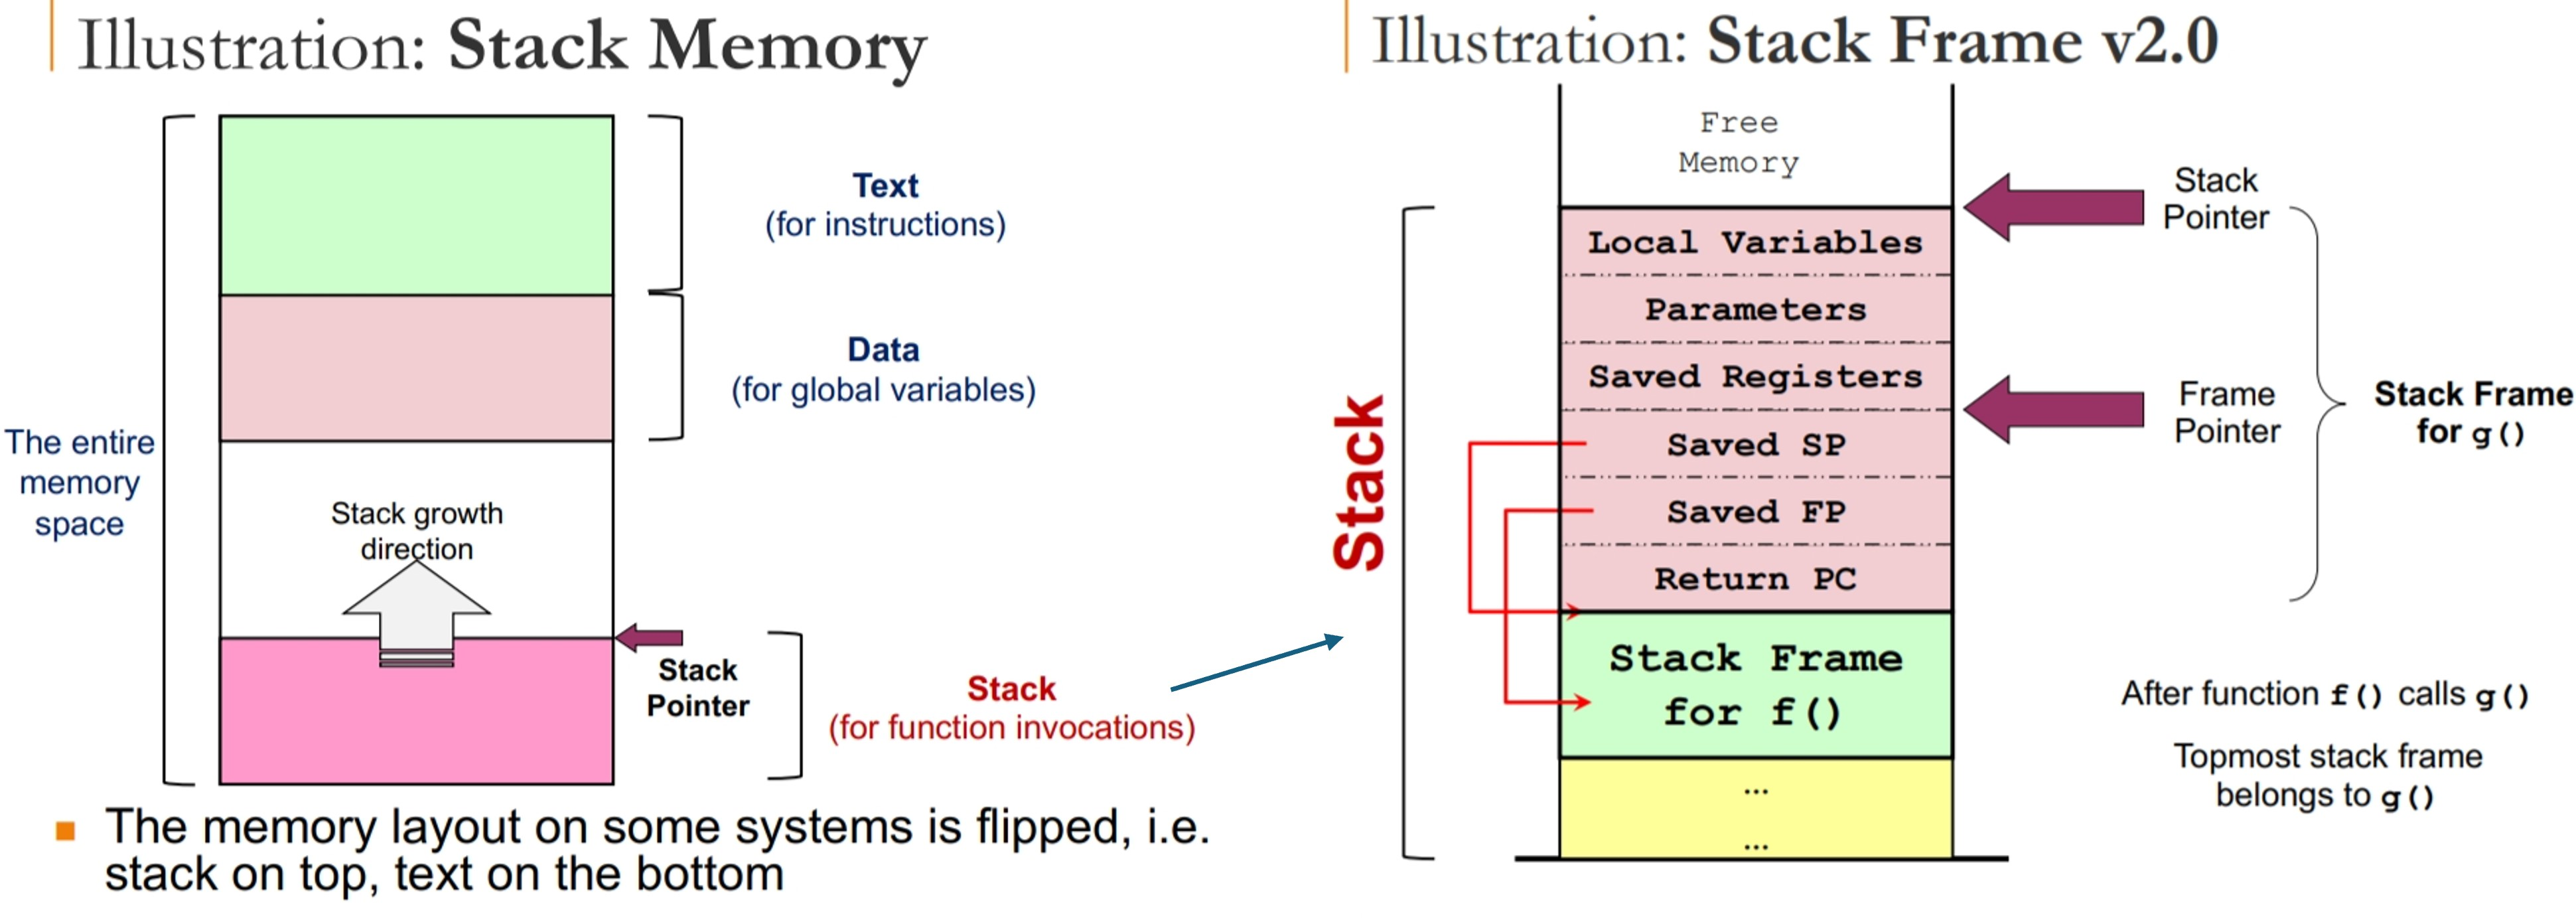
\includegraphics[width=1\linewidth]{stackMemory}}

\subsection{Memory Context for Dynamically Allocated Mem. (Heap)}
Most programming languages allow dynamically allocated memory, i.e. acquire memory space during execution time.
\begin{itemize}
\item In C, \code{malloc()} function call, while C++ / Java: \code{new} keyword.
\item Cannot place in \textit{Data region}, as allocated at runtime, size not known during compilation.
\item Cannot place in \textit{Stack region}, as no definite deallocation time, cannot be freed by garbage collector.
\item Solution: Set up separate \textbf{Heap Memory Region}
\end{itemize}

\columnbreak

\subsubsection{Heap Memory}
\begin{itemize}
\item Managing heap memory trickier due to variable size, variable allocation / deallocation timing.
\item Common situation where heap memory alloc/dealloc creating "holes" in memory. Free memory block squeezed between occupied memory blocks.
\item Covered in memory management.
\end{itemize}
\centerline{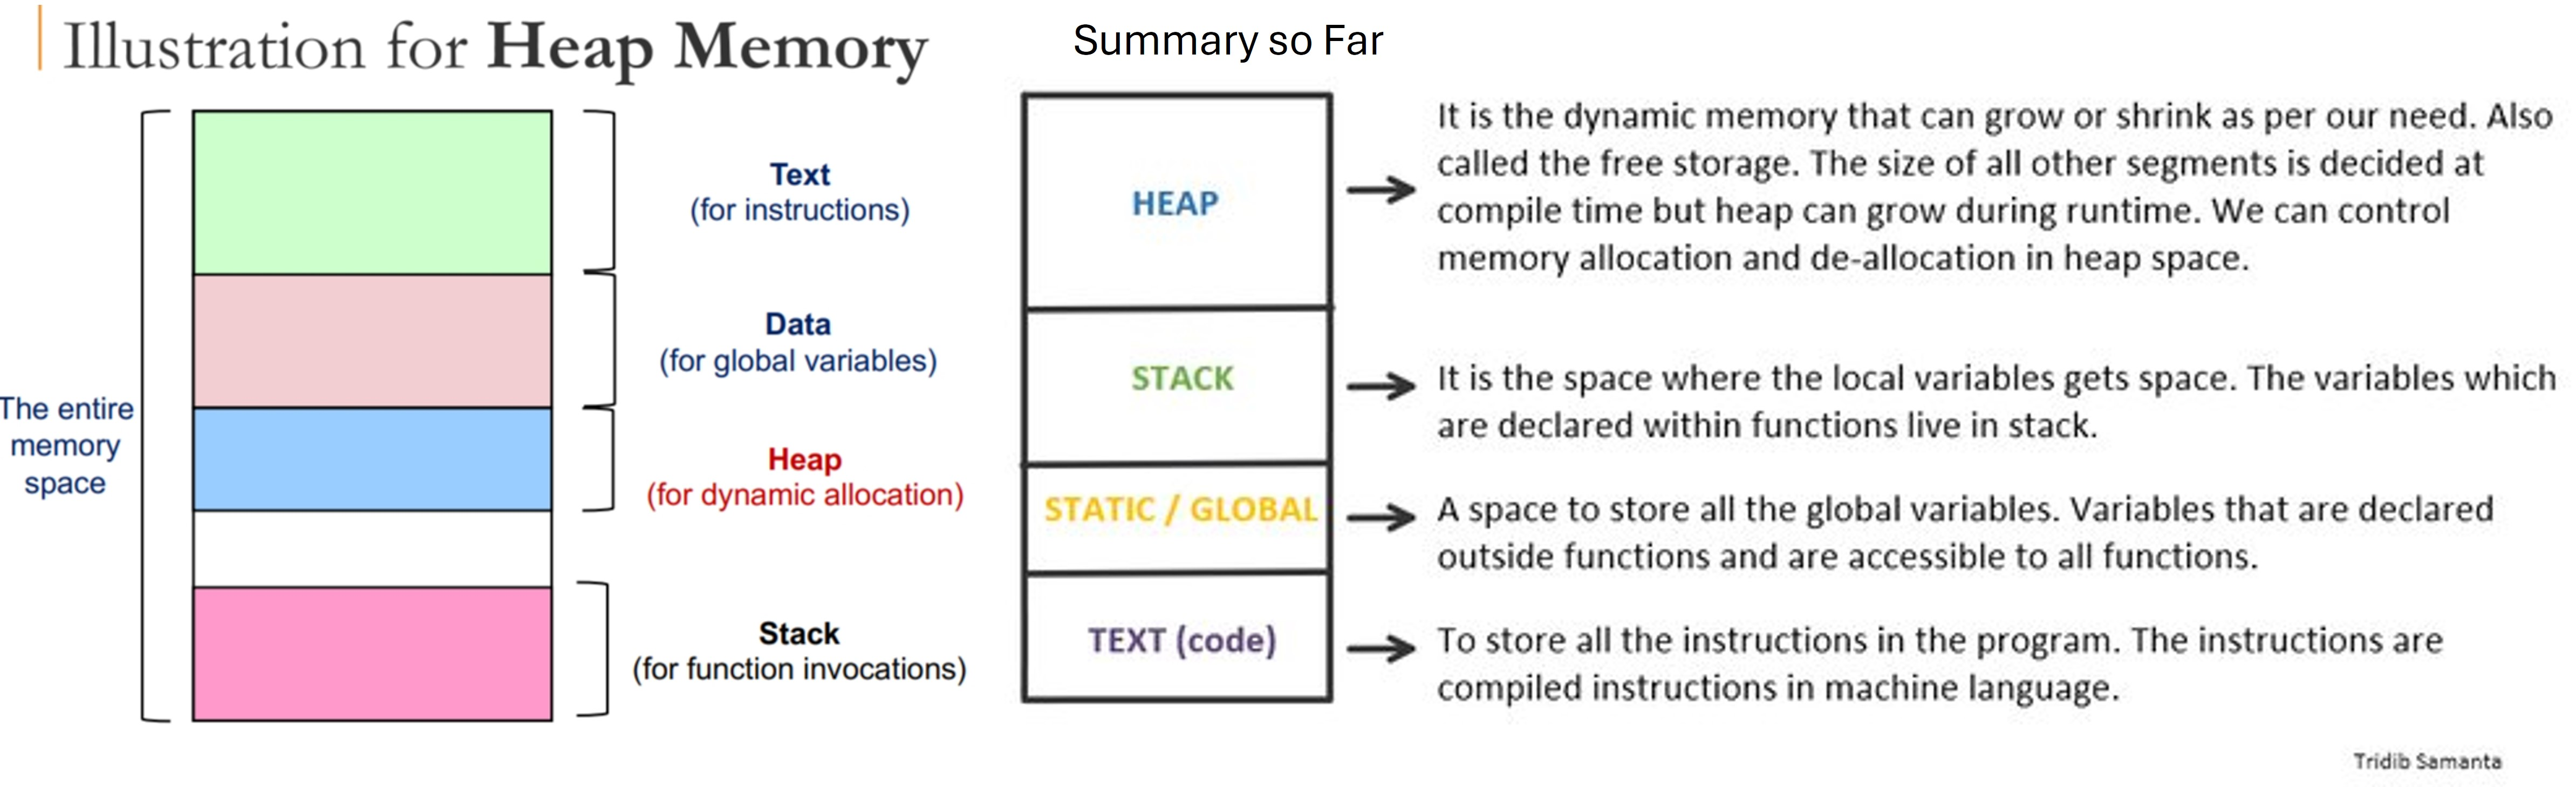
\includegraphics[width=1\linewidth]{heapMemory}}


\subsection{OS Context: Process ID, Process State}
\textbf{Process Identification}:
\begin{itemize}
\item \textbf{Process ID}: To distinguish processes from each other (Just a number, unique among processes)
\item PIDs are OS dependent as well, including if PIDs reused, if limits maximum no. of processes or any PIDs reserved.
\end{itemize}
\textbf{Process State}:
\begin{itemize}
\item Processes require a process state as indication of execution status. (Running / Not Running / Ready to Run etc.)
\item \textbf{Process Model}: Set of states and transitions, describes behaviors of a process.
\item \textbf{Global View of Process States}: Given $n$ processes, \\
- With 1 CPU, $\leq$ 1 process in running state, 1 transition at a time. \\
- With $m$ CPUs, $\leq$ m processes running state, possibly parallel transitions.
\item Different processes may be in different states, each process may be in different part of its state diagram.
\item \textbf{5-State Process Model}: 
\end{itemize}
\centerline{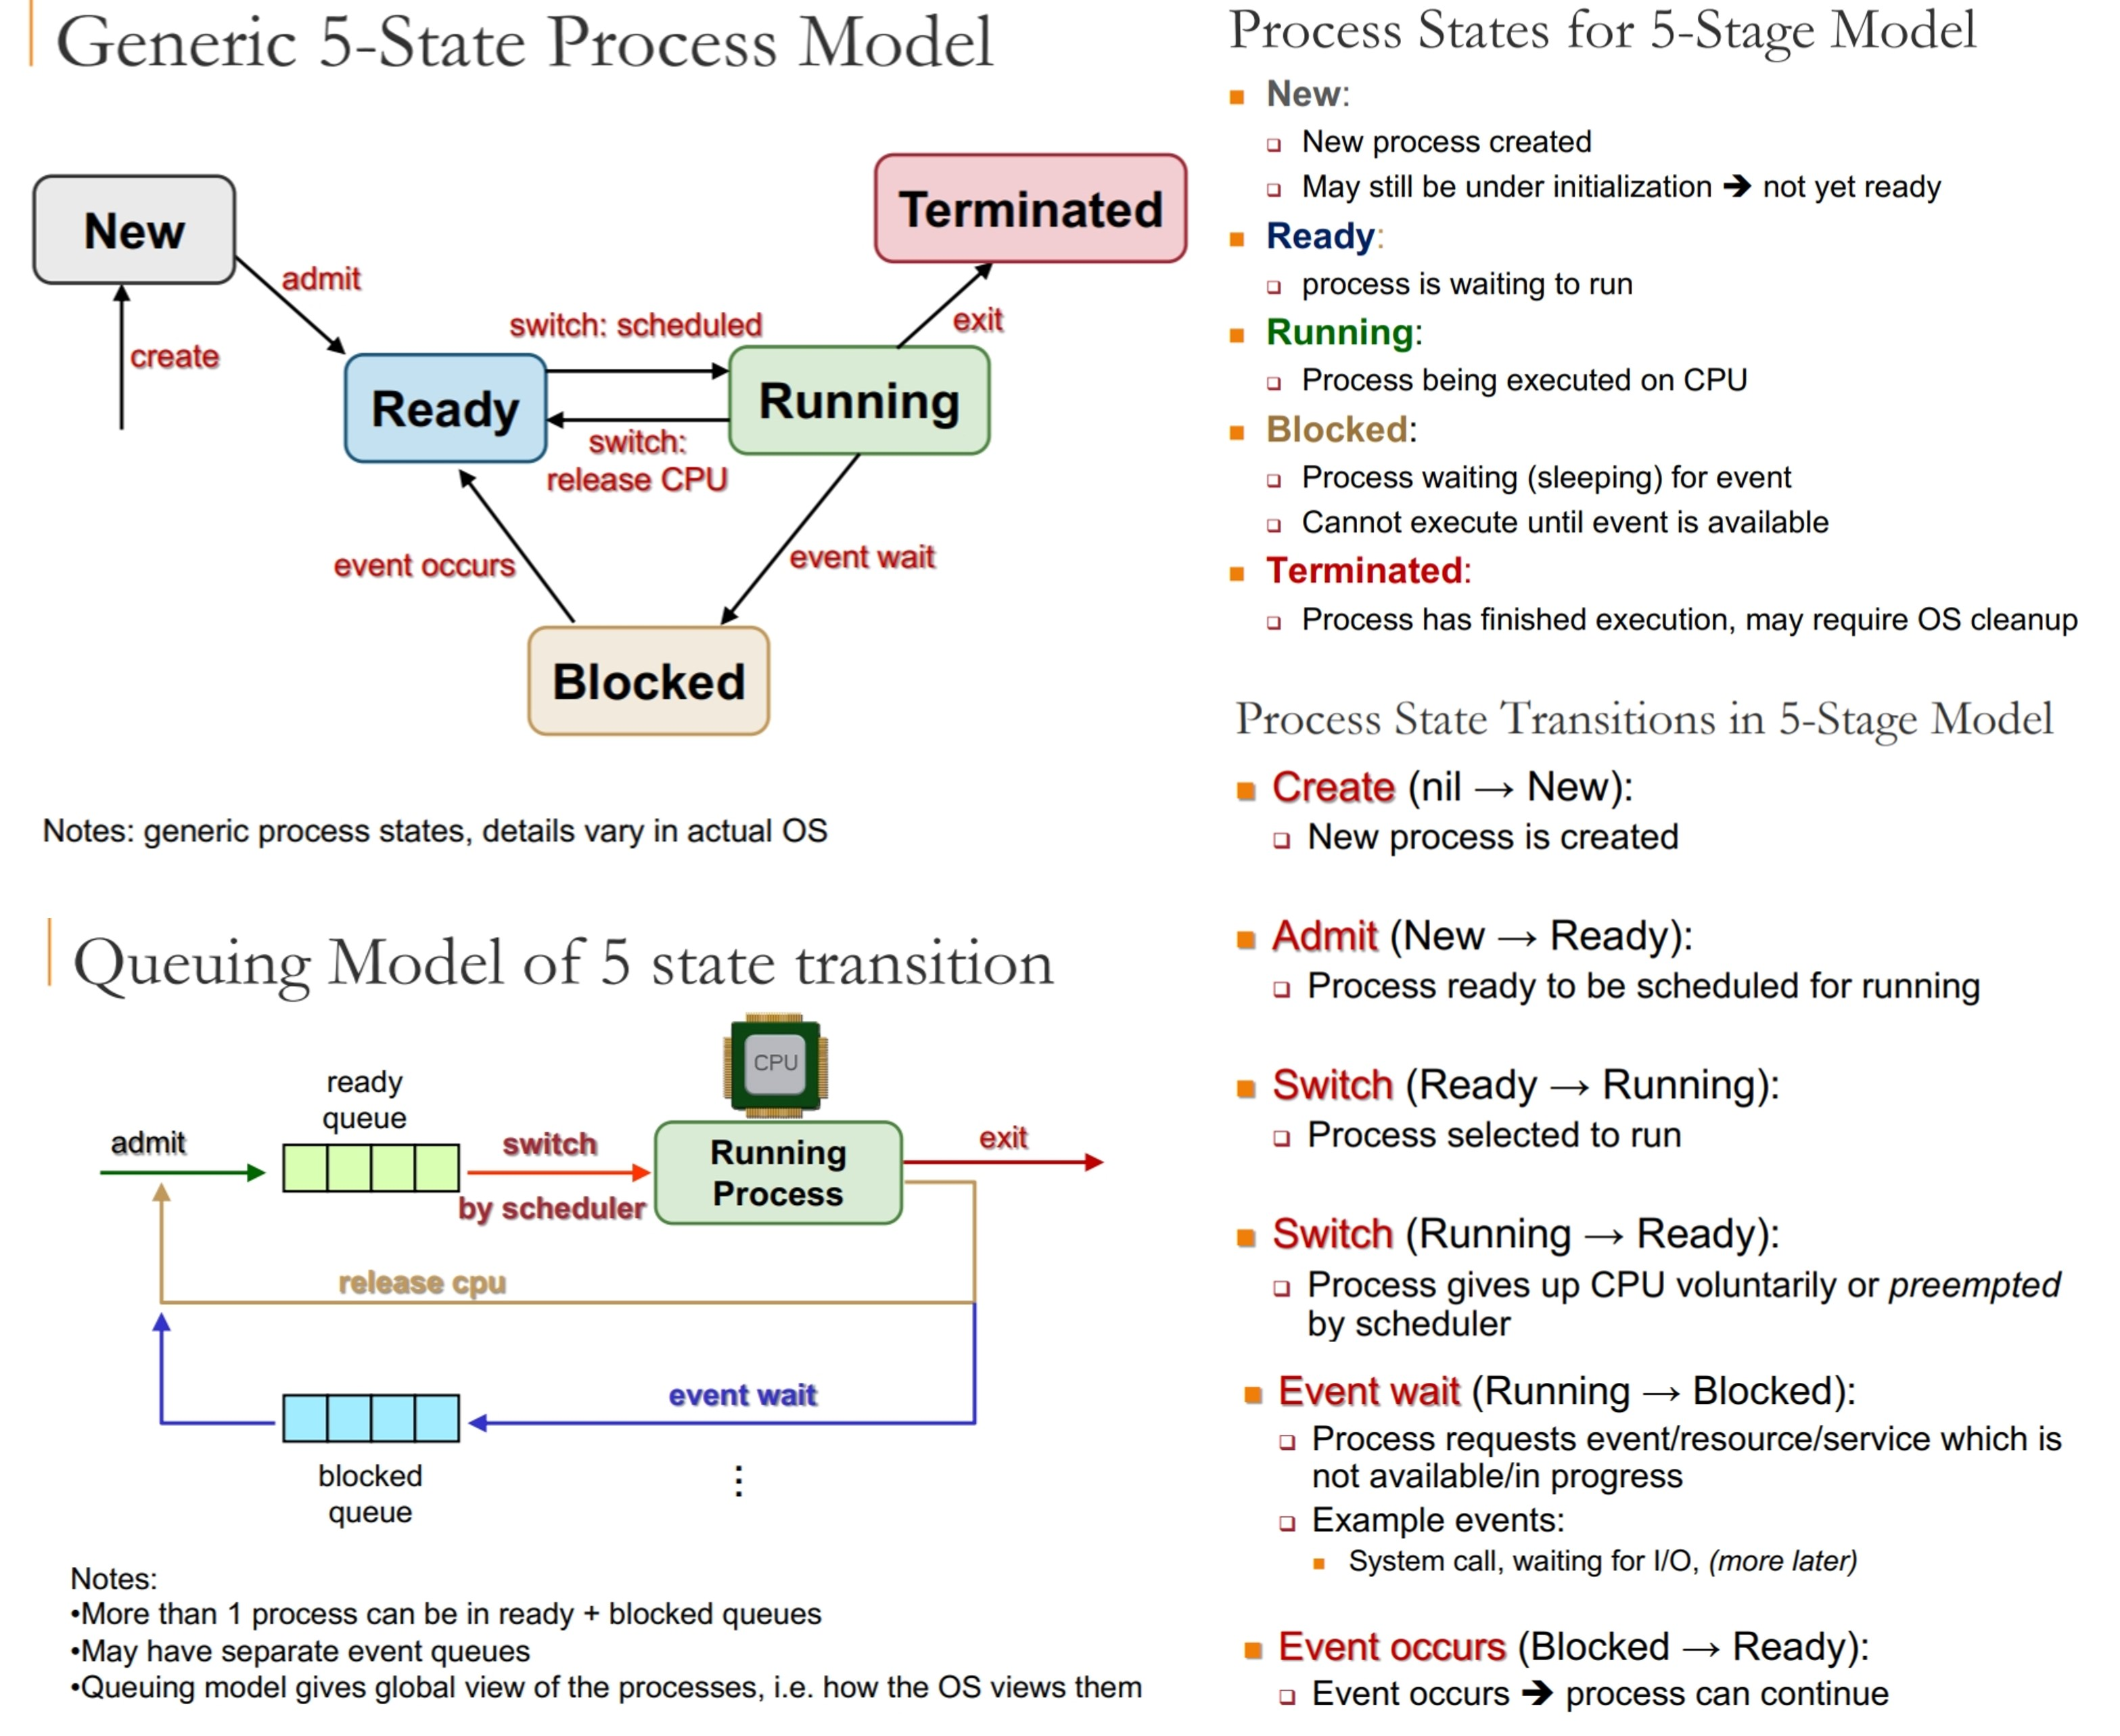
\includegraphics[width=1\linewidth]{5StateProcess}}

\subsection{Process Table \& Process Control Block}
\begin{itemize}
\item Since the OS is just a program as well, need to make use of data structures to track these processes.
\item \textbf{Process Control Block (PCB) or Process Table Entry}: Entire Execution Context for a process.
\item Kernel maintains \textbf{PCB} for all processes. (Conceptually stored as one table representing all processes.)
\item \textbf{Factors to consider}: \\
- Scalability (how many concurrent processes at once). \\
- Efficiency (should provide efficient access with minimum space wastage).
\end{itemize}
\centerline{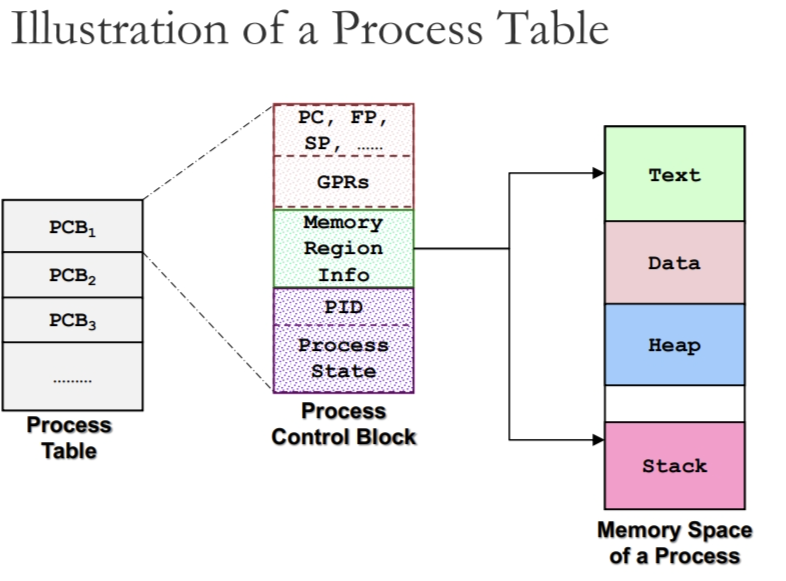
\includegraphics[width=0.6\linewidth]{processTable}}

\subsection{Process Abstraction in Unix}
\begin{itemize}
\item \textbf{Process Identification, Information}
\end{itemize}
\centerline{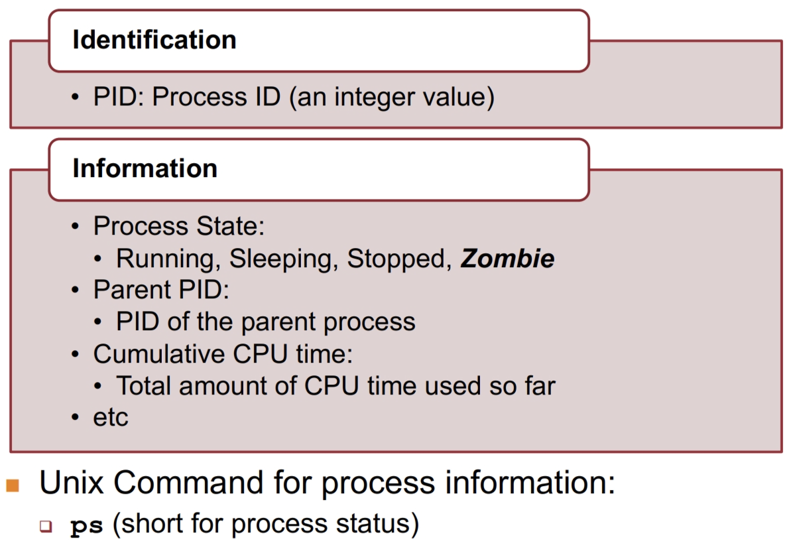
\includegraphics[width=0.6\linewidth]{processAbstraction}}
\begin{itemize}
\item \textbf{Process Creation, Termination, Parent-Child Synchronization}
\end{itemize}

\subsubsection{Note: Command Line Argument in C}
\begin{itemize}
\item We can pass arguments to a program in C.
\item \code{argc}: Number of CL arguments, including program name.
\item \code{argv}: A char strings array, each element in \code{argv[]} is a C character string.
\end{itemize}
\begin{lstlisting} [linewidth = 1.0 \linewidth],
int main( int argc, char* argv[] )
{ int i;
	 for (i = 0; i < argc; i++){
	 printf("Arg \%i: \%s, ",i, argv[i] );
	 }
	 return 0;
}
\end{lstlisting}
\begin{itemize}
\item Example Run: ``a.out 123 hello world''
\item Output: ``Arg 0: a.out, Arg 1: 123, Arg 2: hello, Arg 3: world''
\end{itemize}

\subsubsection{Process Creation: \code{fork()}}
\centerline{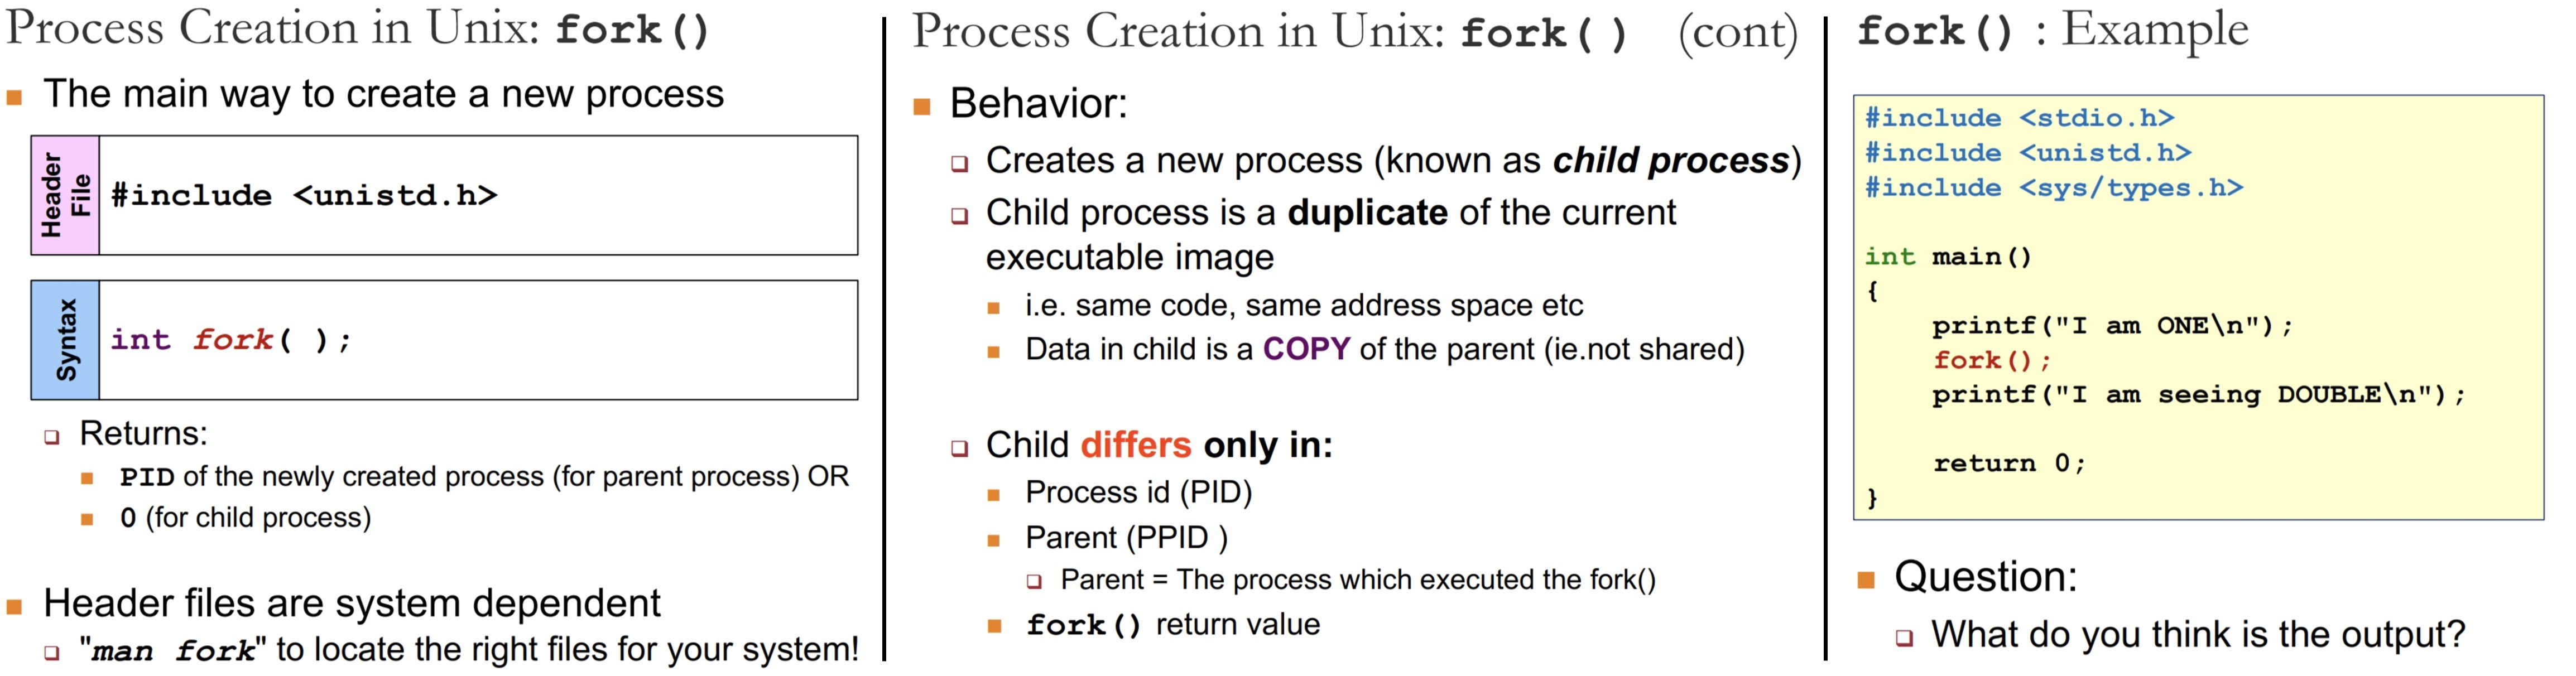
\includegraphics[width=1\linewidth]{processCreation}}
\begin{itemize}
\item \code{fork()}: Create exact copy of the parent, including any variables.
\item \textbf{Output}: Both parent and child resume execution after the point \code{fork()}. 
\item \textbf{Note \code{clone()}}: \code{fork()} not versatile, for scenarios where partial duplication preferred, \code{clone()}, which supersedes \code{fork()}.
\item Both parent and child processes continue executing, common usage is to use the parent/child process differently. (Parent spawn off child to carry out some work, parent ready to take another order.) \\
- Use return value of \code{fork()} to distinguish parent and child.
\end{itemize}
\centerline{\includegraphics[width=0.4\linewidth]{forkResult}}


\subsubsection{Process Replacement: \code{execl()} System Call}
\begin{itemize}
\item Function \textbf{replaces current executing process image} with a new process image specified by path. No return is made because the calling process image is replaced by the new process image.
\item \textbf{Code Replacement}, but \textbf{PID and other information still intact}.
\end{itemize}
\centerline{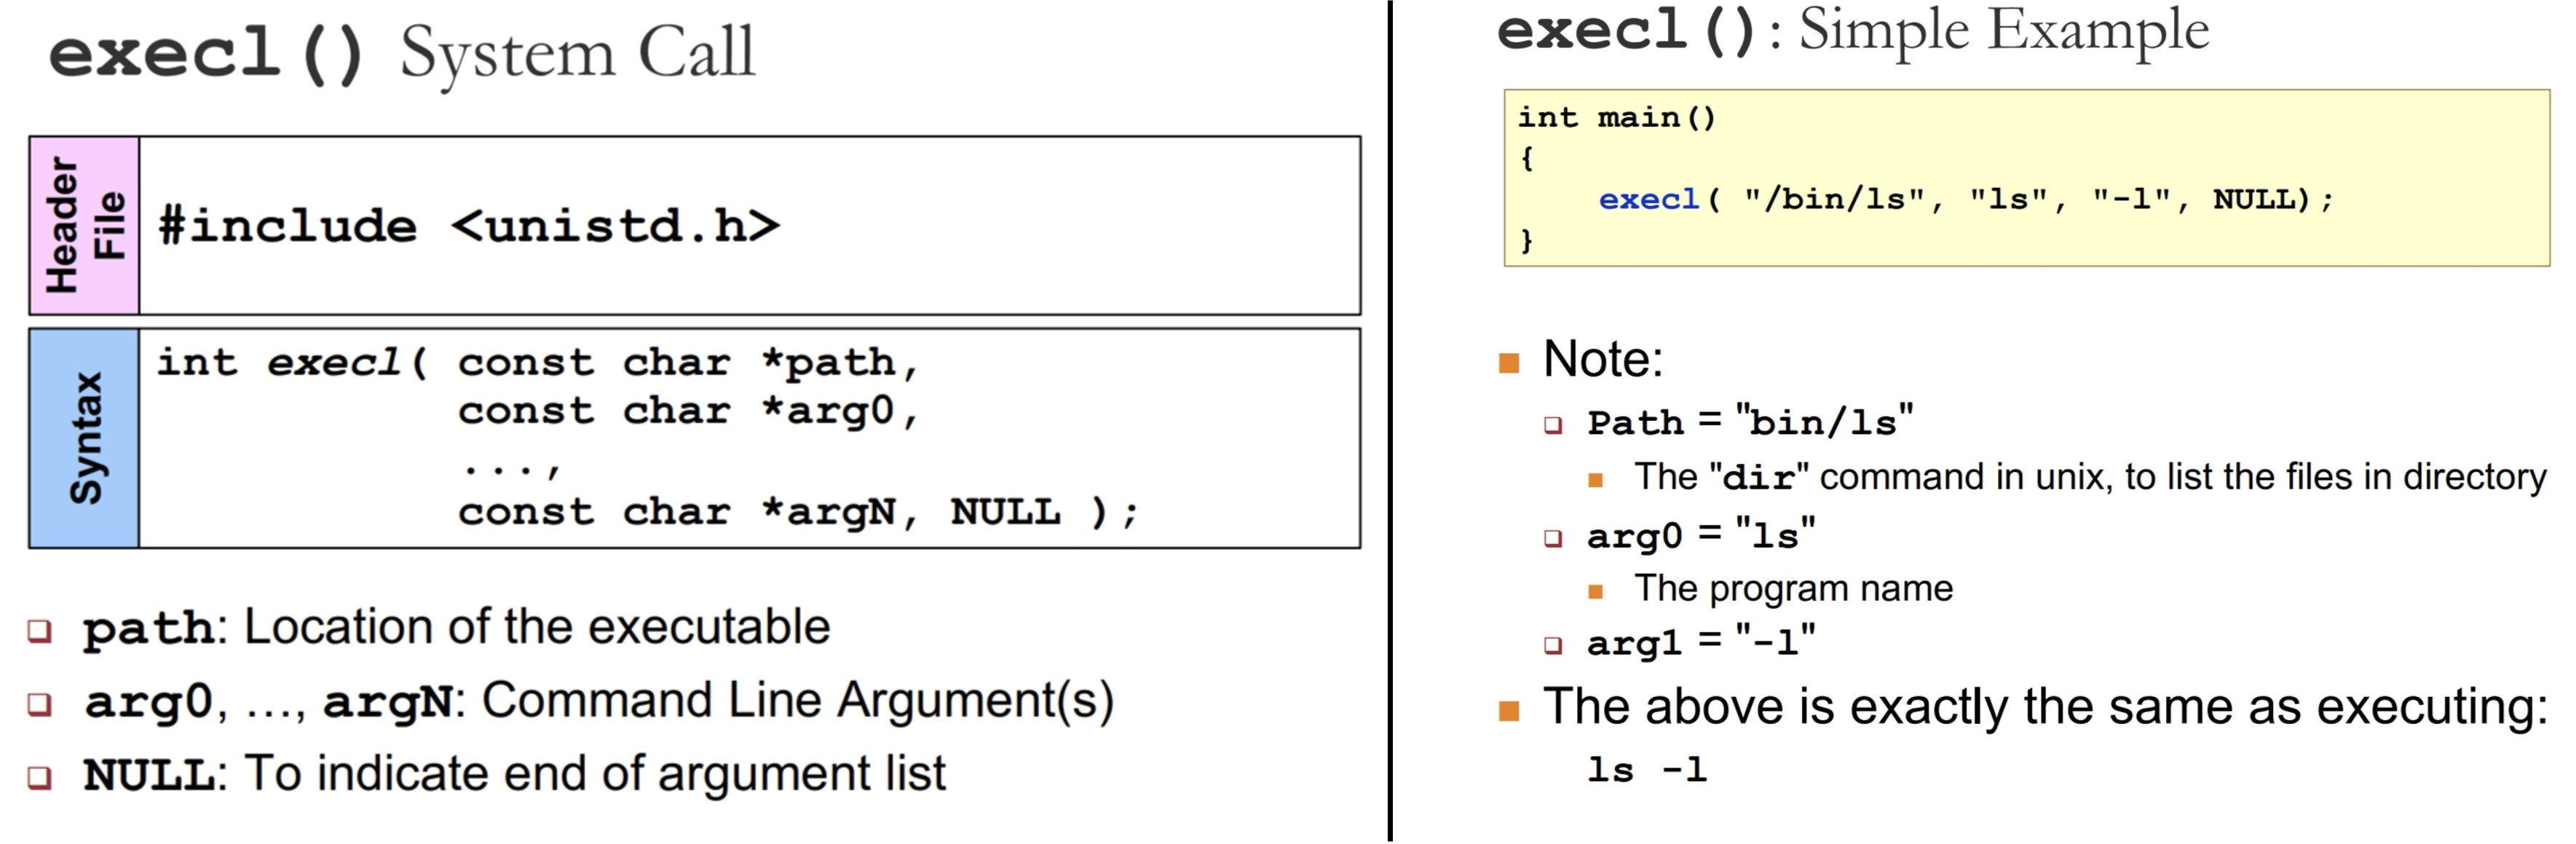
\includegraphics[width=0.95\linewidth]{execl}}
\begin{itemize}
\item \textbf{By combining \code{fork()} and \code{exec()}}, we can spawn off a child process (let it perform task through \code{exec()}), while parent process around to accept another request.
\item This combination of mechanisms is main way in Unix to get new process for running new program!
\end{itemize}

\subsection{The Master Process: \code{init}}
\begin{itemize}
\item Every process has parent process, consider special initial process.
\item \textbf{\code{init} process}: Created in kernel at boot up time, usually PID = 1. 
\item \textbf{Purpose}: Watches and respawns other (critical) processes where needed.
\item \code{fork()} creates the process tree, where \code{init} is the root process.
\end{itemize}

\subsubsection{Simplified Process Tree Ex.}
\centerline{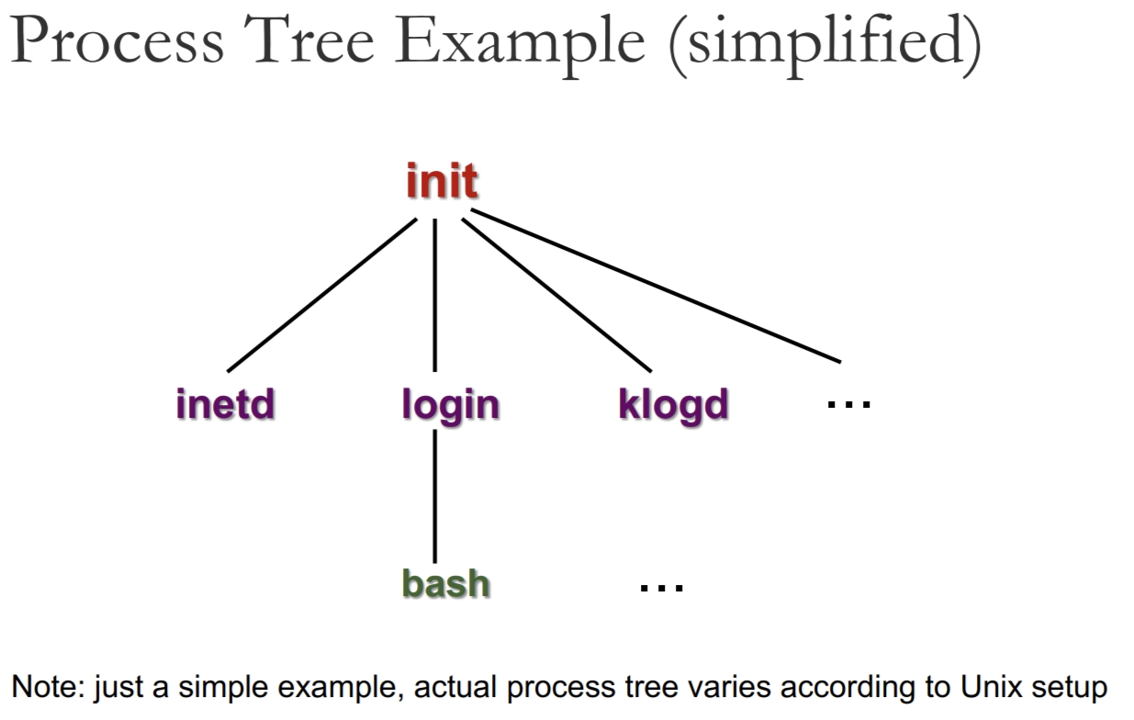
\includegraphics[width=0.6\linewidth]{processTree}}
\begin{itemize}
\item \textbf{d}, (e.g. \code{klogd}) at end of process name usually means server process (Daemon, background process.)
\end{itemize}

\subsubsection{Process Termination in Unix: \code{exit}}
\centerline{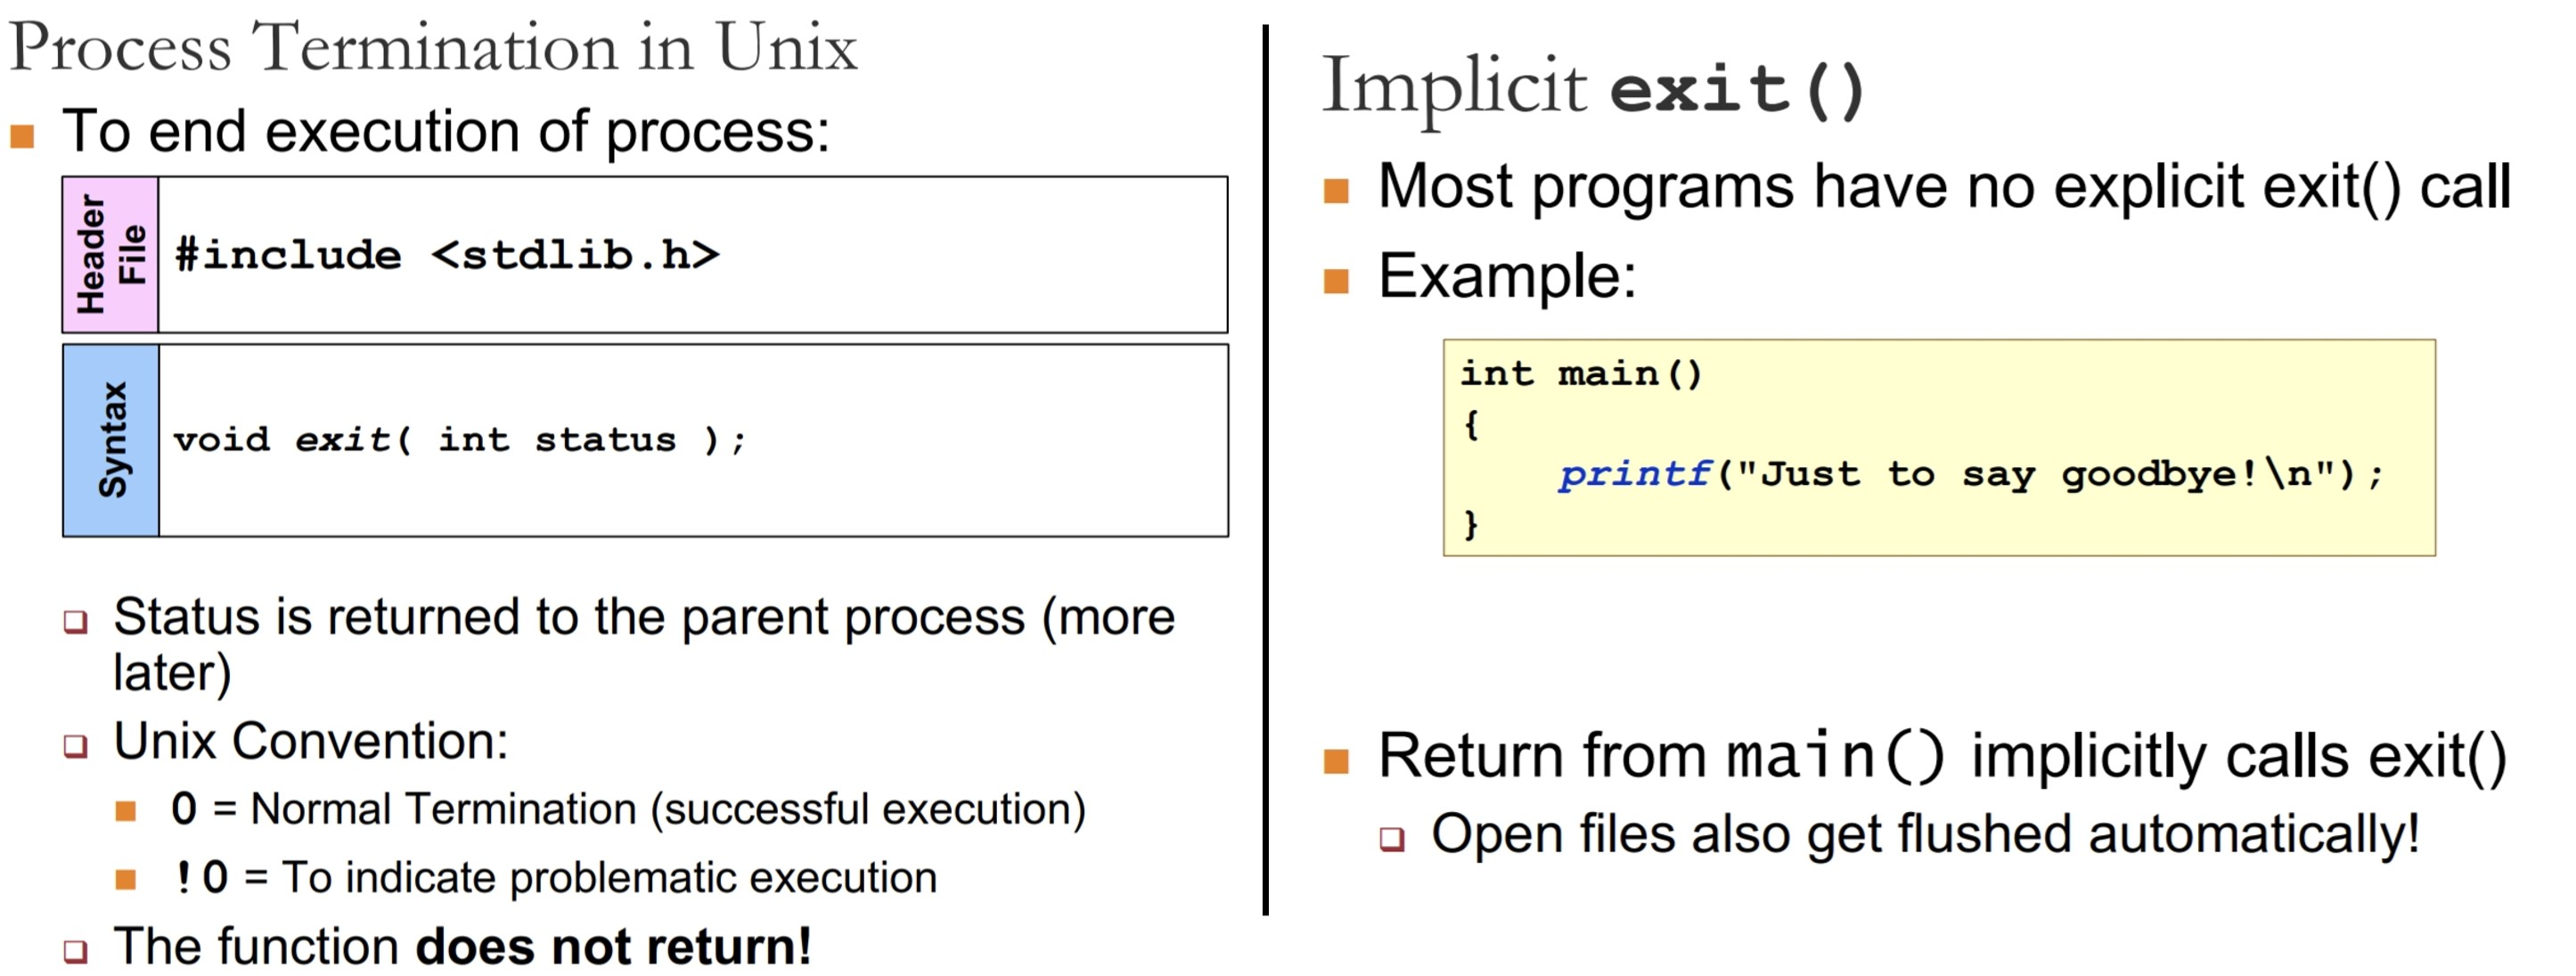
\includegraphics[width=1\linewidth]{processTermination}}
\medskip
\begin{itemize}
\item \textbf{Process finished execution}: \textbf{Most} system resources used by process are released on exit. (e.g. file descriptors).
\item \textbf{Certain basic process resources not Releasable}: PID, status needed. For parent-children synchronization, for parent to check status of child, For process accounting info (e.g. cpu time).
\item Process table entry may still be needed after termination.
\end{itemize}

\subsubsection{Parent/Child Synchronization in Unix}
\begin{itemize}
\item Parent process can wait for child process to terminate.
\item Argument is a pointer to a variable that will store the return value (\code{*status}).
\end{itemize}
\centerline{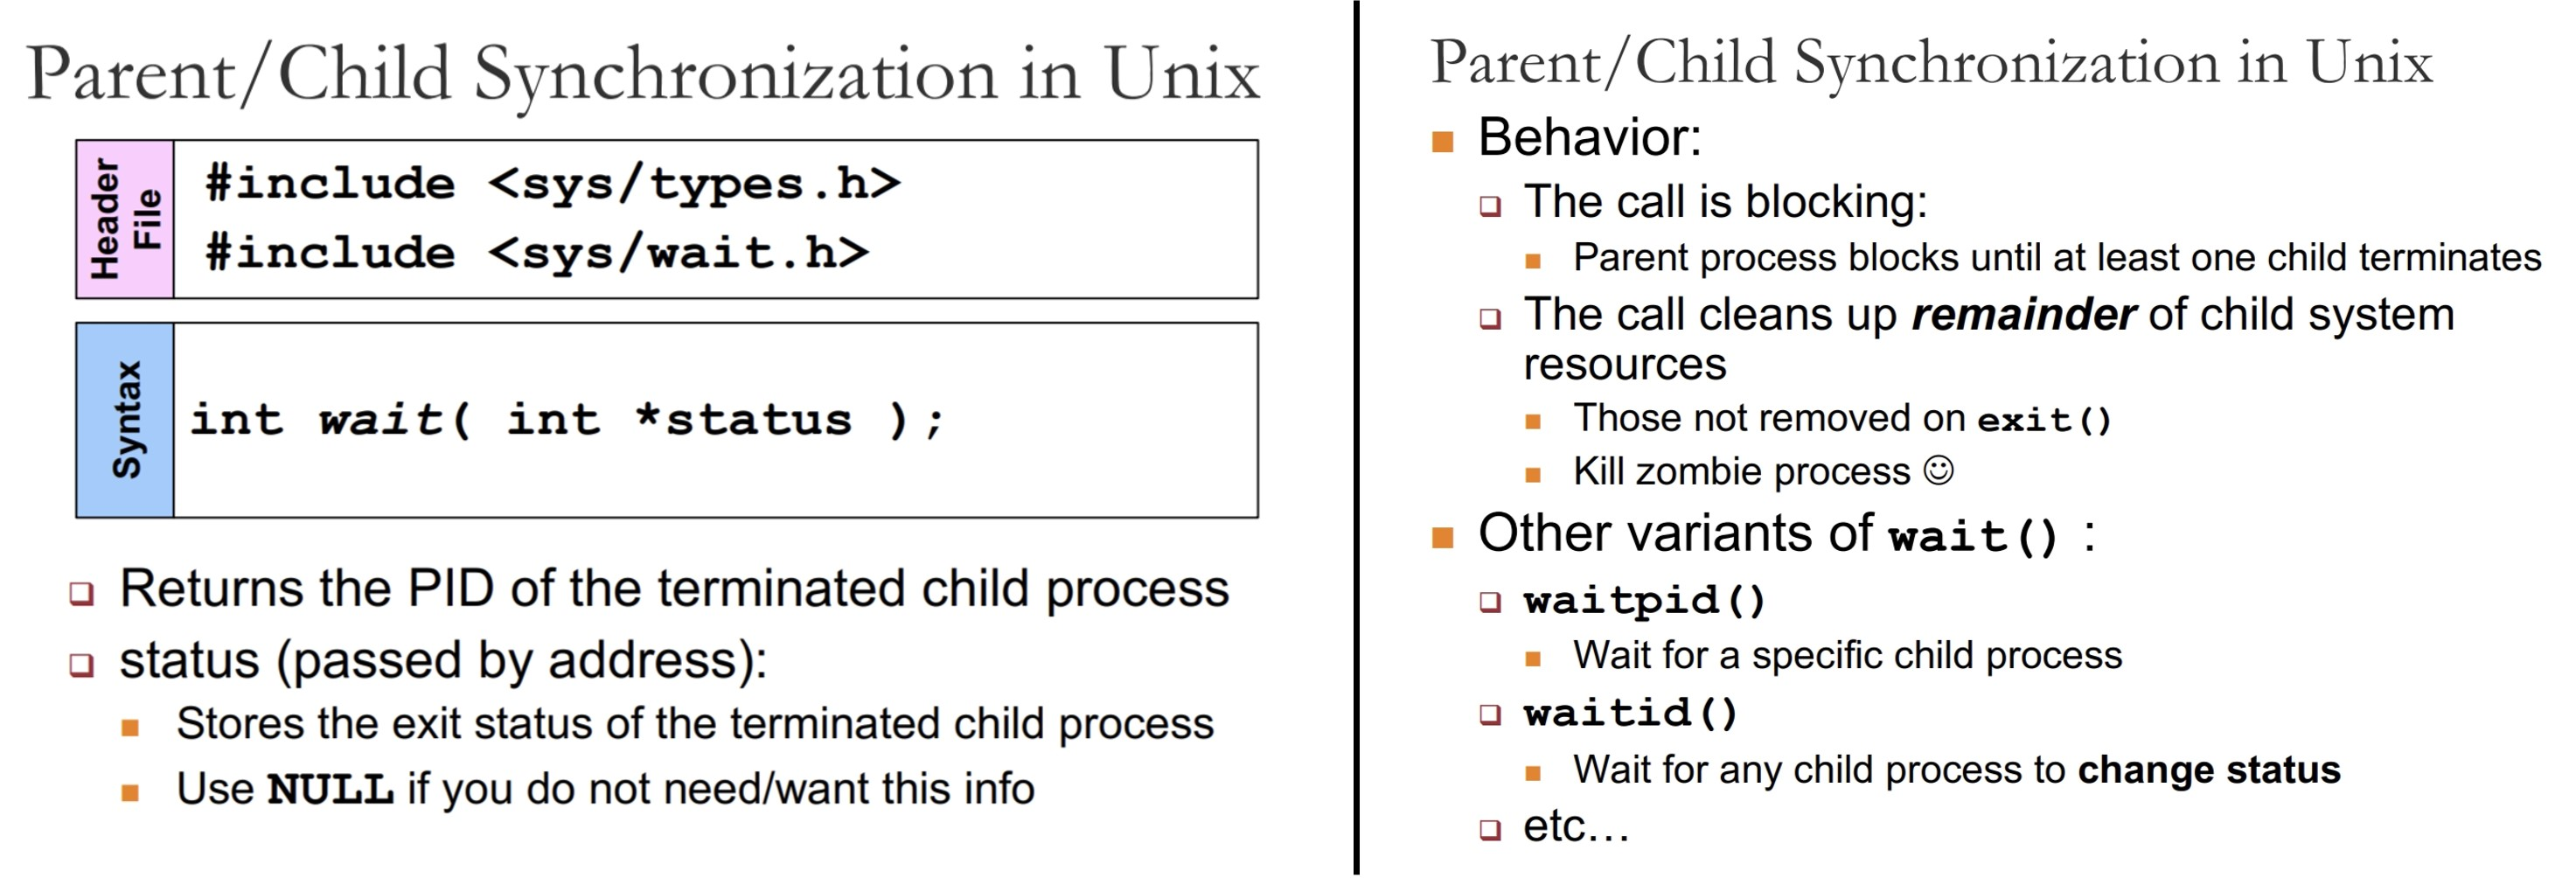
\includegraphics[width=1\linewidth]{PCSynchronization}}
\begin{itemize}
\item Kills zombie processes! With enough zombies, process table finite size, run out of space.
\end{itemize}
\centerline{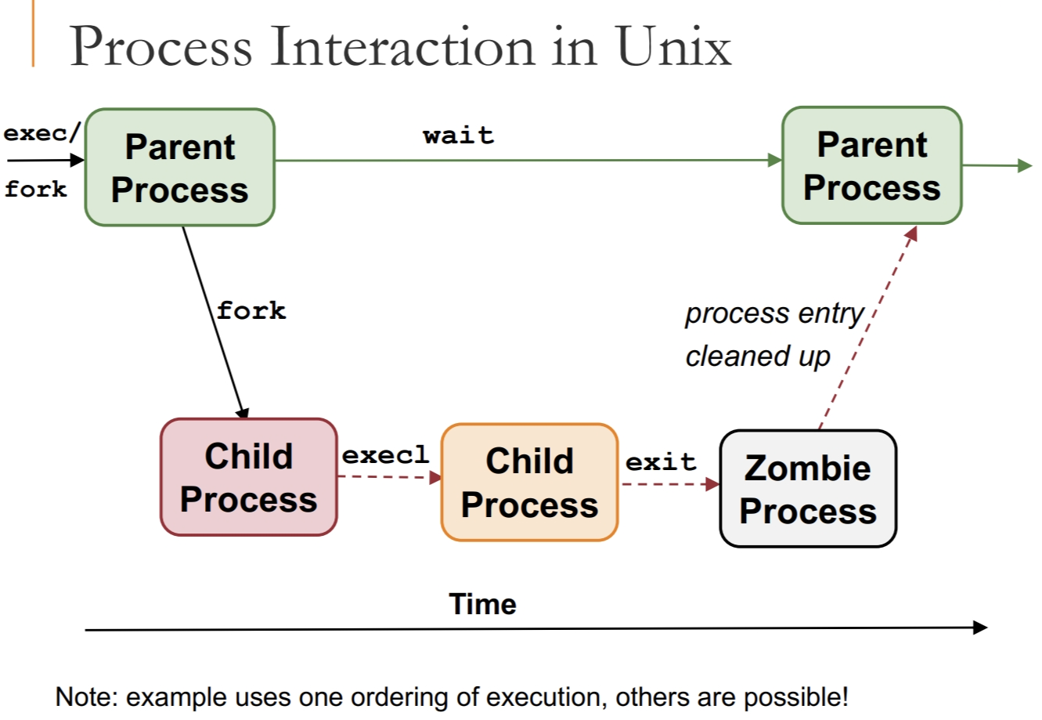
\includegraphics[width=0.5\linewidth]{processInteraction}}

\subsubsection{Zombie Processes (2 Cases)}
\begin{itemize}
\item \code{wait()} ``creates'' the zombies (and later cleans it up) as on process exit, process becomes zombie.
\item Since it cannot delete all process info (if parent asks for info in \code{wait()} call, remainder of process data structure can be cleaned up only when \code{wait()} happens.)
\item We cannot \code{kill PID} zombie process, is already dead. Until restart system or modern OS look through table and remove them.
\end{itemize}

\begin{enumerate}
\item \textbf{Parent process terminates before child process}
	\begin{itemize}
	\item \code{init} process becomes "pseudo" parent of child processes.
	\item Child termination sends signal to \code{init}, which utilizes \code{wait()} to cleanup 
	\end{itemize}
\item \textbf{Child process terminates before parent but parent did not call wait}
	\begin{itemize}
	\item Child process become a zombie process
	\item Can fill up / hog process table, May need a reboot to clear the table on older Unix implementations
	\end{itemize}
\end{enumerate}
\centerline{\includegraphics[width=1\linewidth]{processSummary}}

\section{Implementation Issues}
\subsection{Implementing \code{fork()}}
\centerline{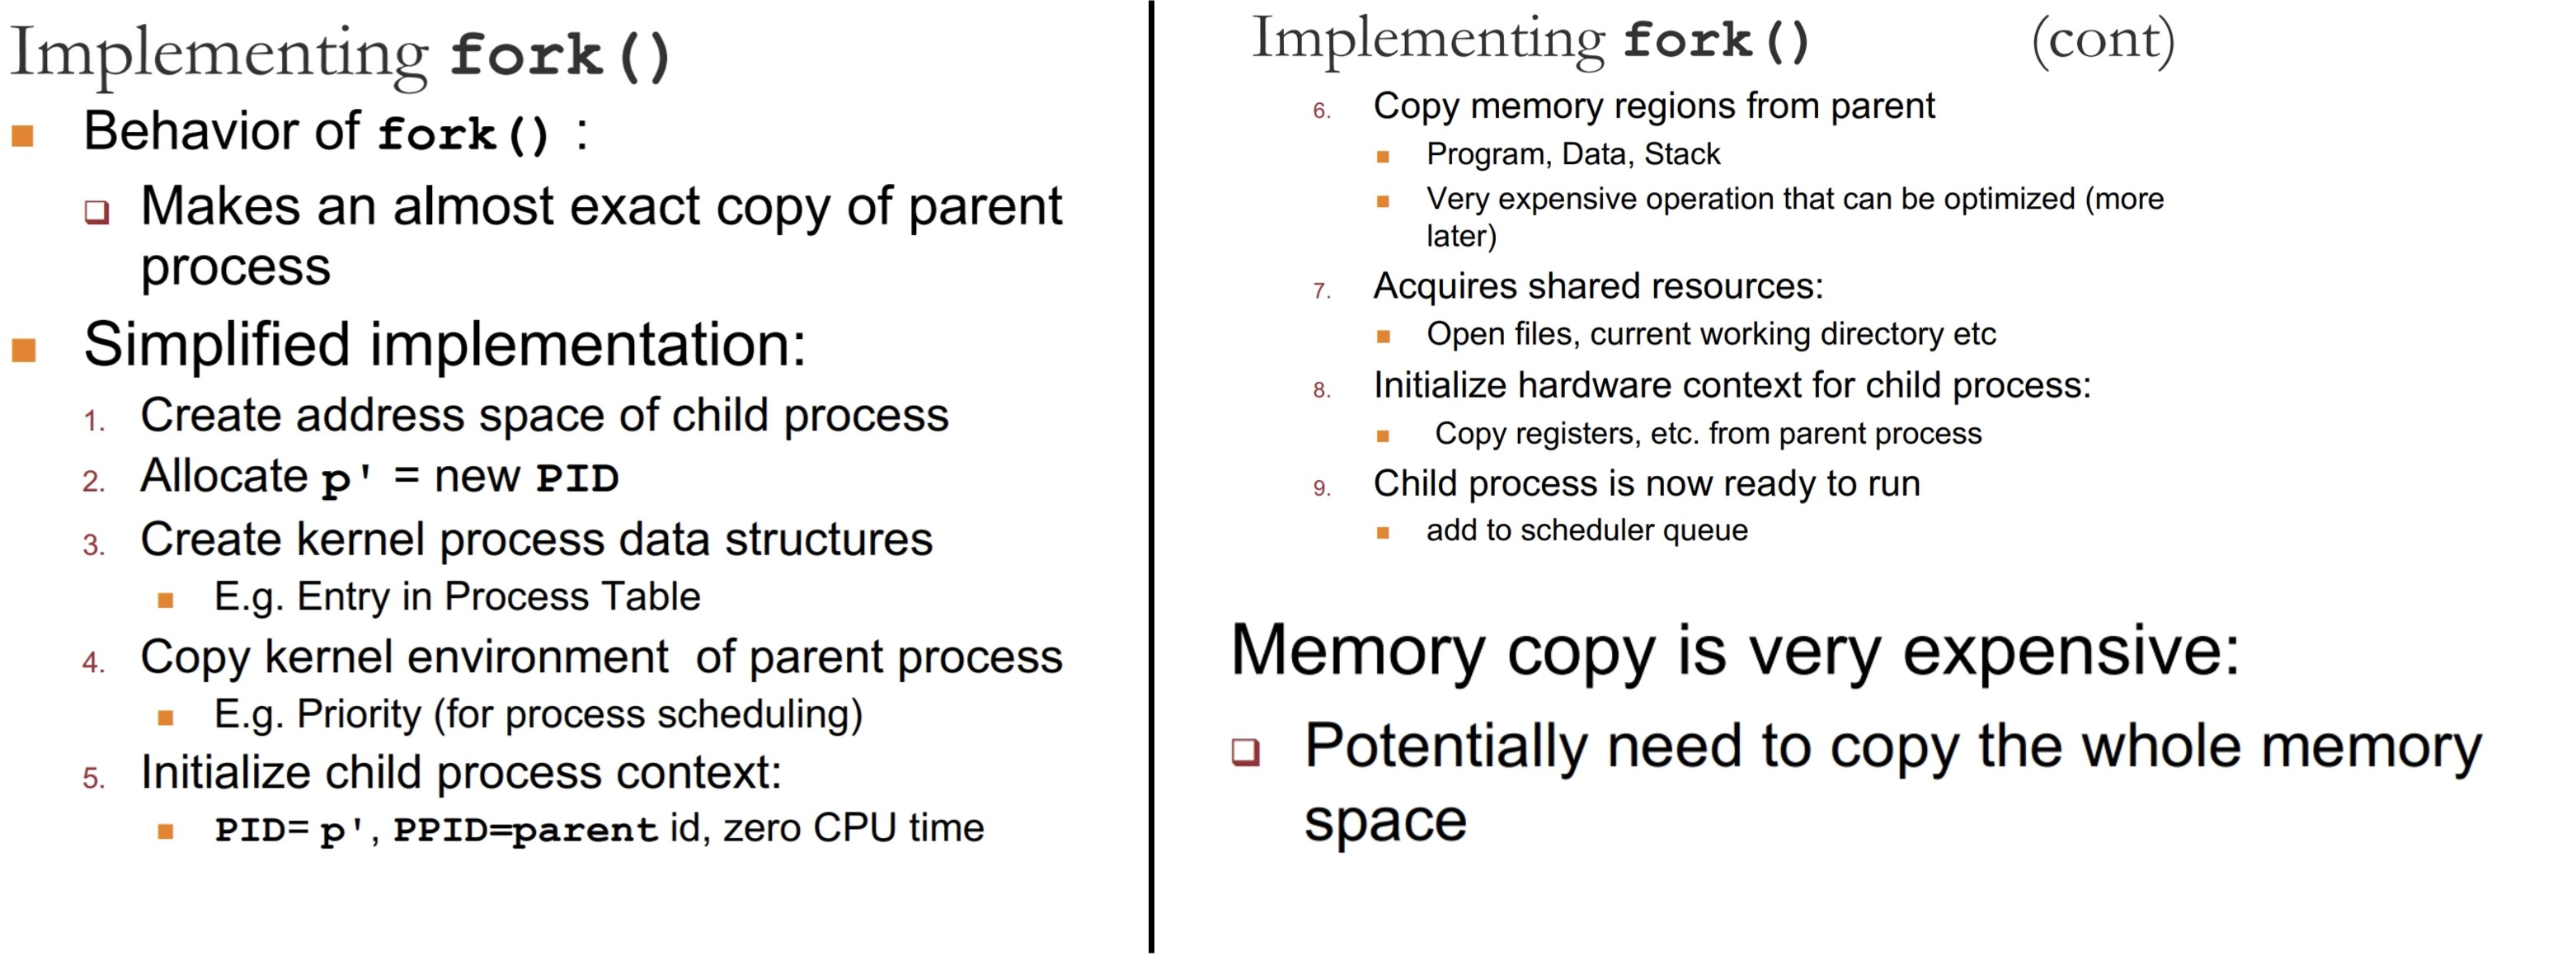
\includegraphics[width=0.95\linewidth]{implementFork}}
\begin{itemize}
\item \textbf{Copying entire memory space is wasteful} and not always needed! (E.g. copy entire 200mb program image of Zoom etc). Mostly, only need contents, and PC, register values.
\item \textbf{Give Rise to COW.} (copy on write)
\end{itemize}

\subsection{Memory Copy Operation}
\begin{itemize}
\item If child just read from location, unchanged, just use a shared version.
\item \textbf{Only when write is perform on a location, then two independent copies needed.}
\item \textbf{Copy on Write} is possible optimization, only duplicate ``memory location'' when it is written to, otherwise parent and child share same ``memory location''.
\item Note: memory organized into memory pages (consec range of mem locations), memory managed on page level instead of individual location.
\end{itemize}

\section{System Calls (Process Interaction with OS)}
\subsection{API to OS: Application Program Interface to OS}
\begin{itemize}
\item OS API provides way of calling facilities/services in kernel.
\item \textbf{Not same as normal function call}: Change from \textit{user mode to kernel mode}.
\item Different OS have different APIs: Unix Variants most follow POSIX standards, small no. of calls ~100. Windows family uses Win API across diff. windows, huge no. of calls ~1000.
\end{itemize}

\subsection{Unix System Calls in C/C++ program}
\begin{itemize}
\item In C/C++ program, \textbf{system call can be invoked almost directly}, as library version very closely reflects these calls.
\item Majority of system calls have library version with \textbf{same name} and parameters, library version acts as \textbf{function wrapper}. 
\item A few library functions present more user friendly version, e.g. less no. /more flexible parameters). Library version acts as \textbf{function adapter}.
\end{itemize}
\centerline{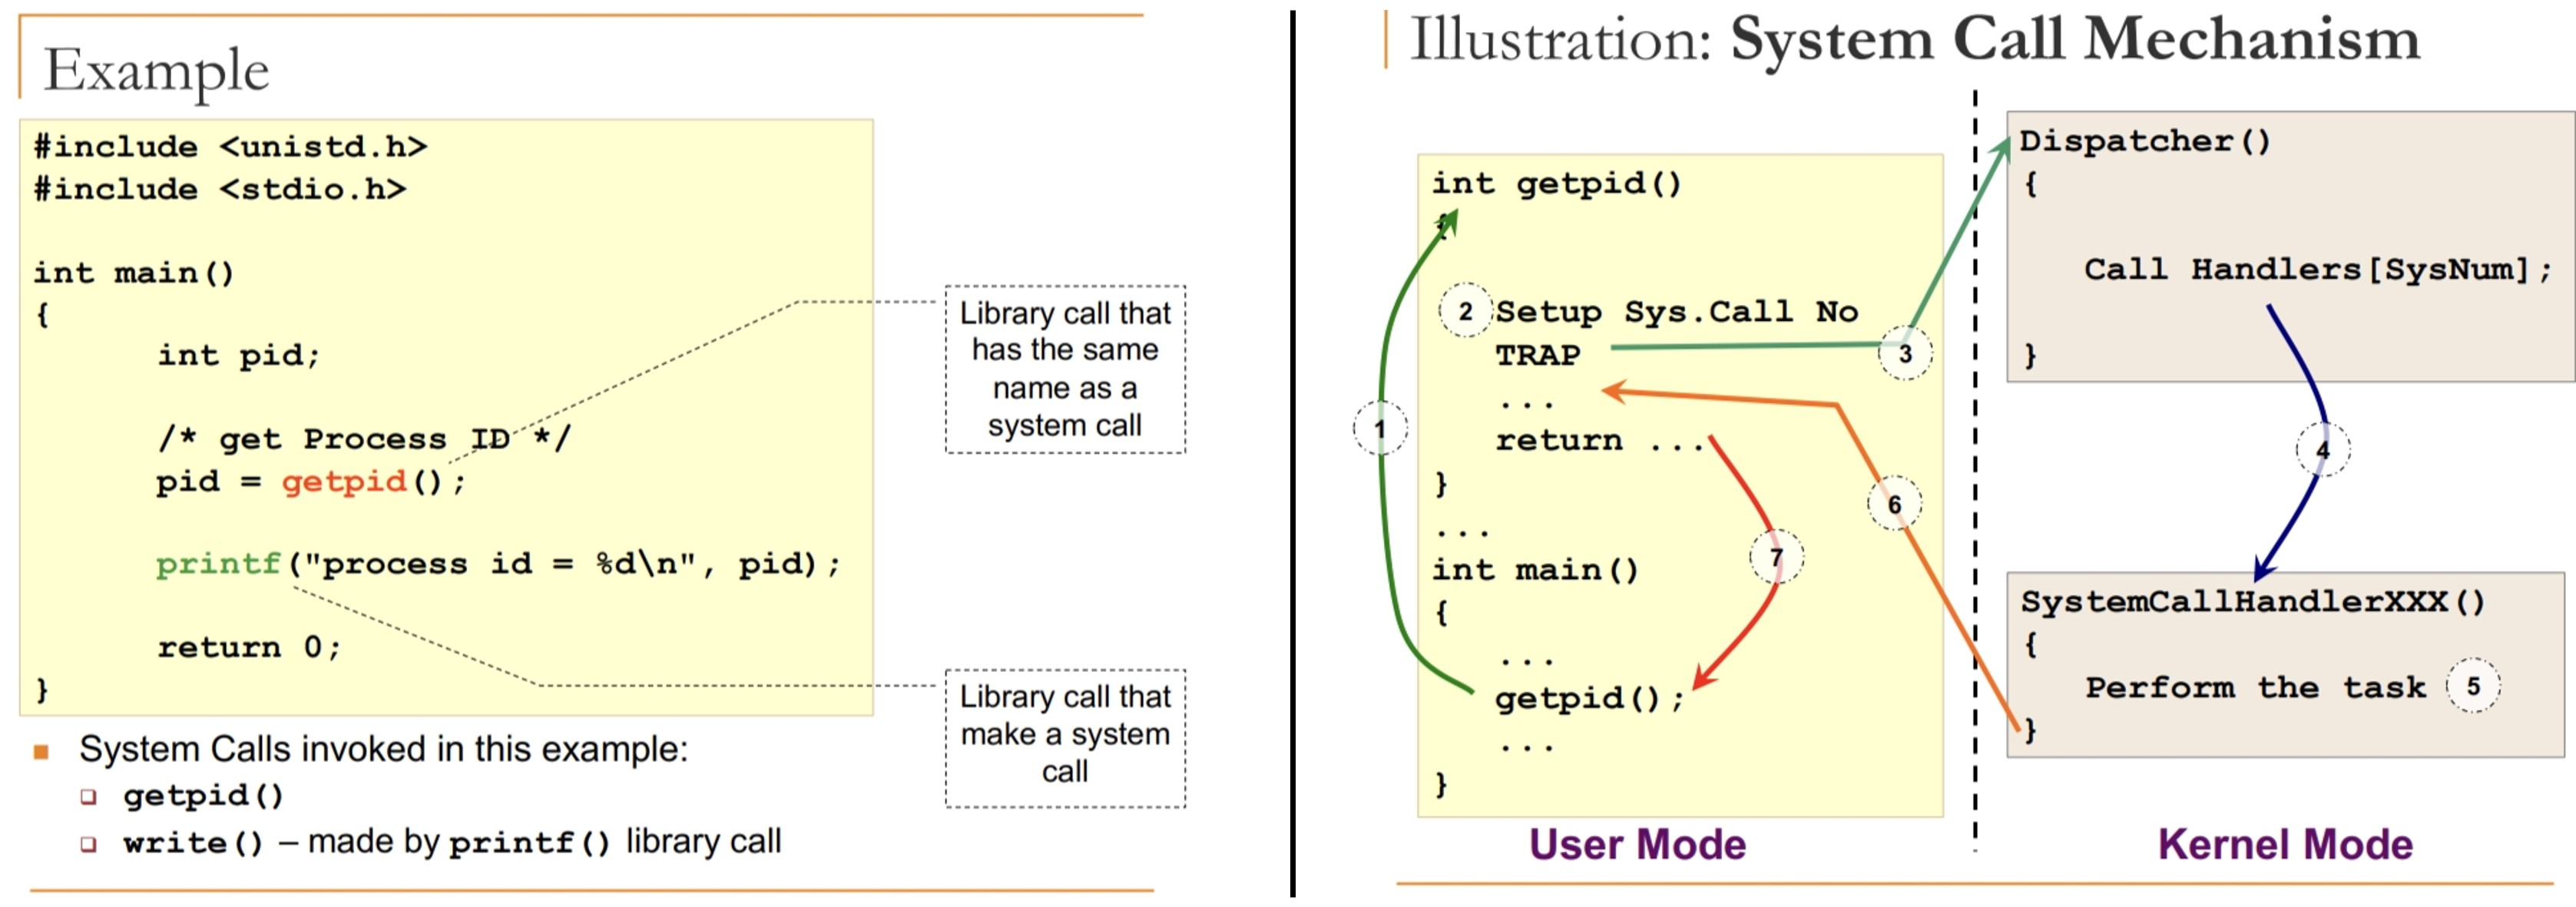
\includegraphics[width=1\linewidth]{systemCallExample}}

\subsection{General System Call Mechanism}
\centerline{\includegraphics[width=1\linewidth]{generalSystemCallMechanism}}

\section{Exception and Interrupt}

\subsubsection{Exception}
\begin{itemize}
\item \textbf{Executing machine level instruction} can cause \textbf{exception}. For example:
\begin{itemize}
\item Airthmetic Errors: Overflow, Underflow, Division by Zero
\item Memory Accessing Errors: (accessing memory not belonging to program), Illegal memory address, mis-aligned memory access.
\end{itemize}
\item Exception is \textbf{Synchronous}: Determinate, occurs due to program execution at exact points of time.
\item \textbf{Effect of Exception}: Have to execute \textbf{exception handler}, which is similar to a \textbf{``forced function call''!}
\item Exception $\neq$ Interrupt!
\end{itemize}

\columnbreak

\subsubsection{Interrupt}
\begin{itemize}
\item \textbf{External events} can interrupt the execution of a program.
\item Interrupt request lines connected to CPU, lines are checked during instruction execution cycle.
\item Usually hardware related, e.g.: Timer, Mouse move, Keyboard press etc
\item Interrupt is \textbf{asynchronous}: Events occurs independent of program execution.
\item \textbf{Effect of interrupt:} Program execution, suspended, execute an interrupt handler.
\end{itemize}
\centerline{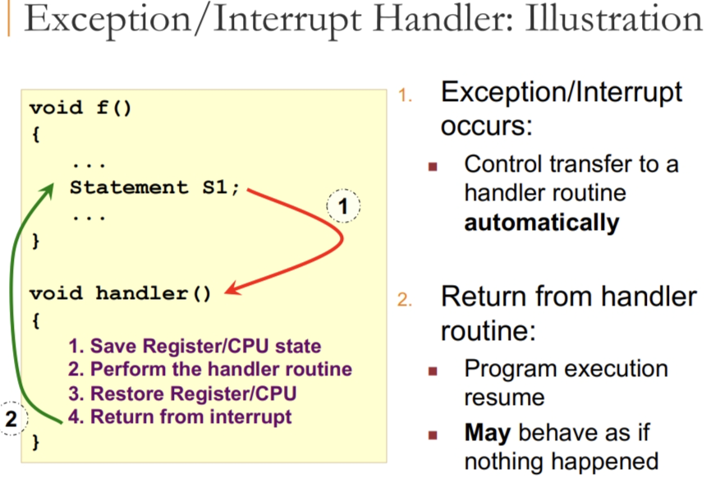
\includegraphics[width=0.5\linewidth]{ExceptionHandler}}

\subsection{Summary}
\begin{itemize}
\item Using \textbf{process as an abstraction} of running program.
\item Includes necessary information (environment) of execution, Memory, Hardware and OS contexts.
\item \textbf{Process from OS perspective}: PCB and process table
\item \textbf{How OS \& Process interact}: System calls, Exception / Interrupt
\end{itemize}

\subsubsection{REFER TO TEXTBOOK:}
\begin{itemize}
\item \textbf{Modern Operating System (3rd Edition)}
\begin{itemize}
\item Section 2.1: Processes
\item Section 2.4: Process Scheduling
\item Section 2.2: Threads
\end{itemize}
\item \textbf{Operating System Concepts (8th Edition)}
\item Section 3.1
\end{itemize}

\vfill \null
\columnbreak

\section{3. Process Scheduling}
A multiprogrammed computer frequently has multiple processes/threads computing for CPU at the same time. Occurs whenever $\geq$ 2 simultaneously in ready state. 
\begin{itemize}
\item \textbf{Scheduler}: Part of OS to decide which process to run next.
\item \textbf{Scheduling Algorithm}: Algo used.
\item \textbf{Scheduling Problem}: Choosing, ready process $>$ available CPUs.
\item In addition to picking right process, need \textbf{efficient use of CPU} as process switching is expensive. (Switch user to kernel mode, save state of process, memory map, memory cache may need to reload, etc.)
\item \textbf{I/O Input/Output} (disk or network): When process enters blocked state waiting for external device to complete work.
\end{itemize}

\subsubsection{Process Behavior}
\begin{itemize}
\item Process' unique \textbf{requirement of CPU time.}
\item Process goes through phases of CPU-activity \& IO-activity.
\item \textbf{Compute/CPU-Bound Process} (computation, e.g. number crunching) vs. \textbf{IO-bound Process} (e.g. read/write to file, print to screen)
\end{itemize}
\centerline{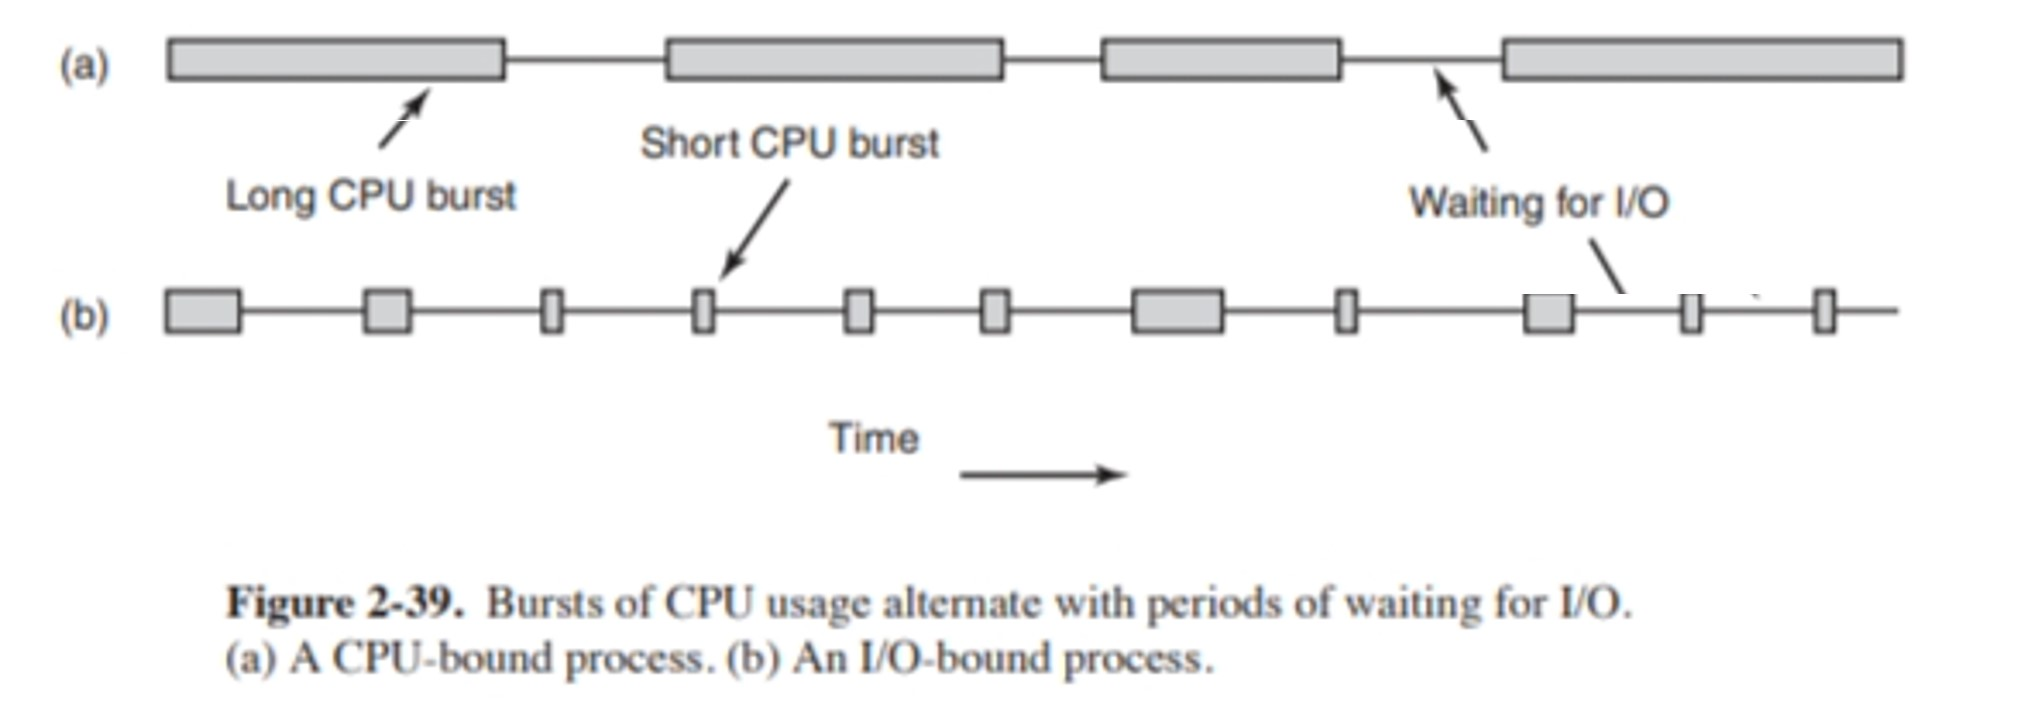
\includegraphics[width=0.7\linewidth]{processBehavior}}

\subsubsection{Process Environment}
\begin{itemize}
\item \textbf{Batch Processing}: No user, no interaction / responsiveness required.
\item \textbf{Interactive / Multiprogramming}: Active user interacting with system. Need responsive, consistent in response time.
\item \textbf{Real Time Processing}: Deadline to meet, usually periodic process.
\end{itemize}

\subsection{Scheduler Evaluation Criteria}
\begin{itemize}
\item Many criteria to evaluating algo, largely influenced by p. environment. May be conflicting.
\item \textbf{All Systems}: \\
- \textit{Fairness}: CPU time (per process basis / per user basis). \textbf{No starvation}. \\
- \textit{Balance}: All parts of computing system utilized.
\item \textbf{Batch Systems}: \\
- \textit{Throughput}: Maximize jobs per hour. \\
- \textit{Turnaround time}: Minimize time btwn. submission \& termination. \\ 
- \textit{++(Waiting Time)}: Related to turnaround, time waiting for CPU \\
- \textit{CPU utilization}: keep CPU busy all the time.
\item \textbf{Interactive Systems}: \\
- \textit{Response time}: respond to requests quickly. \\
- \textit{Proportionality}: meet users' expectations.
\item \textbf{Real-time Systems}: \\
- \textit{Meeting deadlines}: avoid losing data. (e.g. livestream)\\
- \textit{Predictability}: avoid quality degradation in multimedia.
\end{itemize}

\subsection{Concurrent Execution}
\begin{itemize}
\item \textbf{Concurrent Processes}: Logical concept to cover multitasked processes.
\item \textbf{Virtual parallelism}: Illusion of parallelism (pseudo-parallelism)
\item \textbf{Physical parallelism}: Multiple CPUs/Cores, multiple parallel exec
\end{itemize}


\columnbreak

\subsection{When to Schedule}
Key issue, when to make schedule decisions. \\
E.g. When new process created, run parent or child. When process exits, when process blocks on I/O, or I/O interrupt.
\begin{itemize}
\item \textbf{Non-preemptive (cooperative)}: Process stays scheduled (running state) until it blocks, or gives up CPU voluntarily.
\item \textbf{Preemptive (Fixed Quota)}: Process given fixed time quota to run (possible to block / give up early). At end of quota, running process suspended, another picked if available.
\end{itemize}


\subsubsection{Interleaved Execution (Timeslicing)}
\begin{itemize}
\item \textbf{Concurrent Execution on 1 CPU}: Interleave instructions from both processes.
\item \textbf{OS overhead}: Multitasking needs to change context between programs, incurs overhead.
\end{itemize}
\centerline{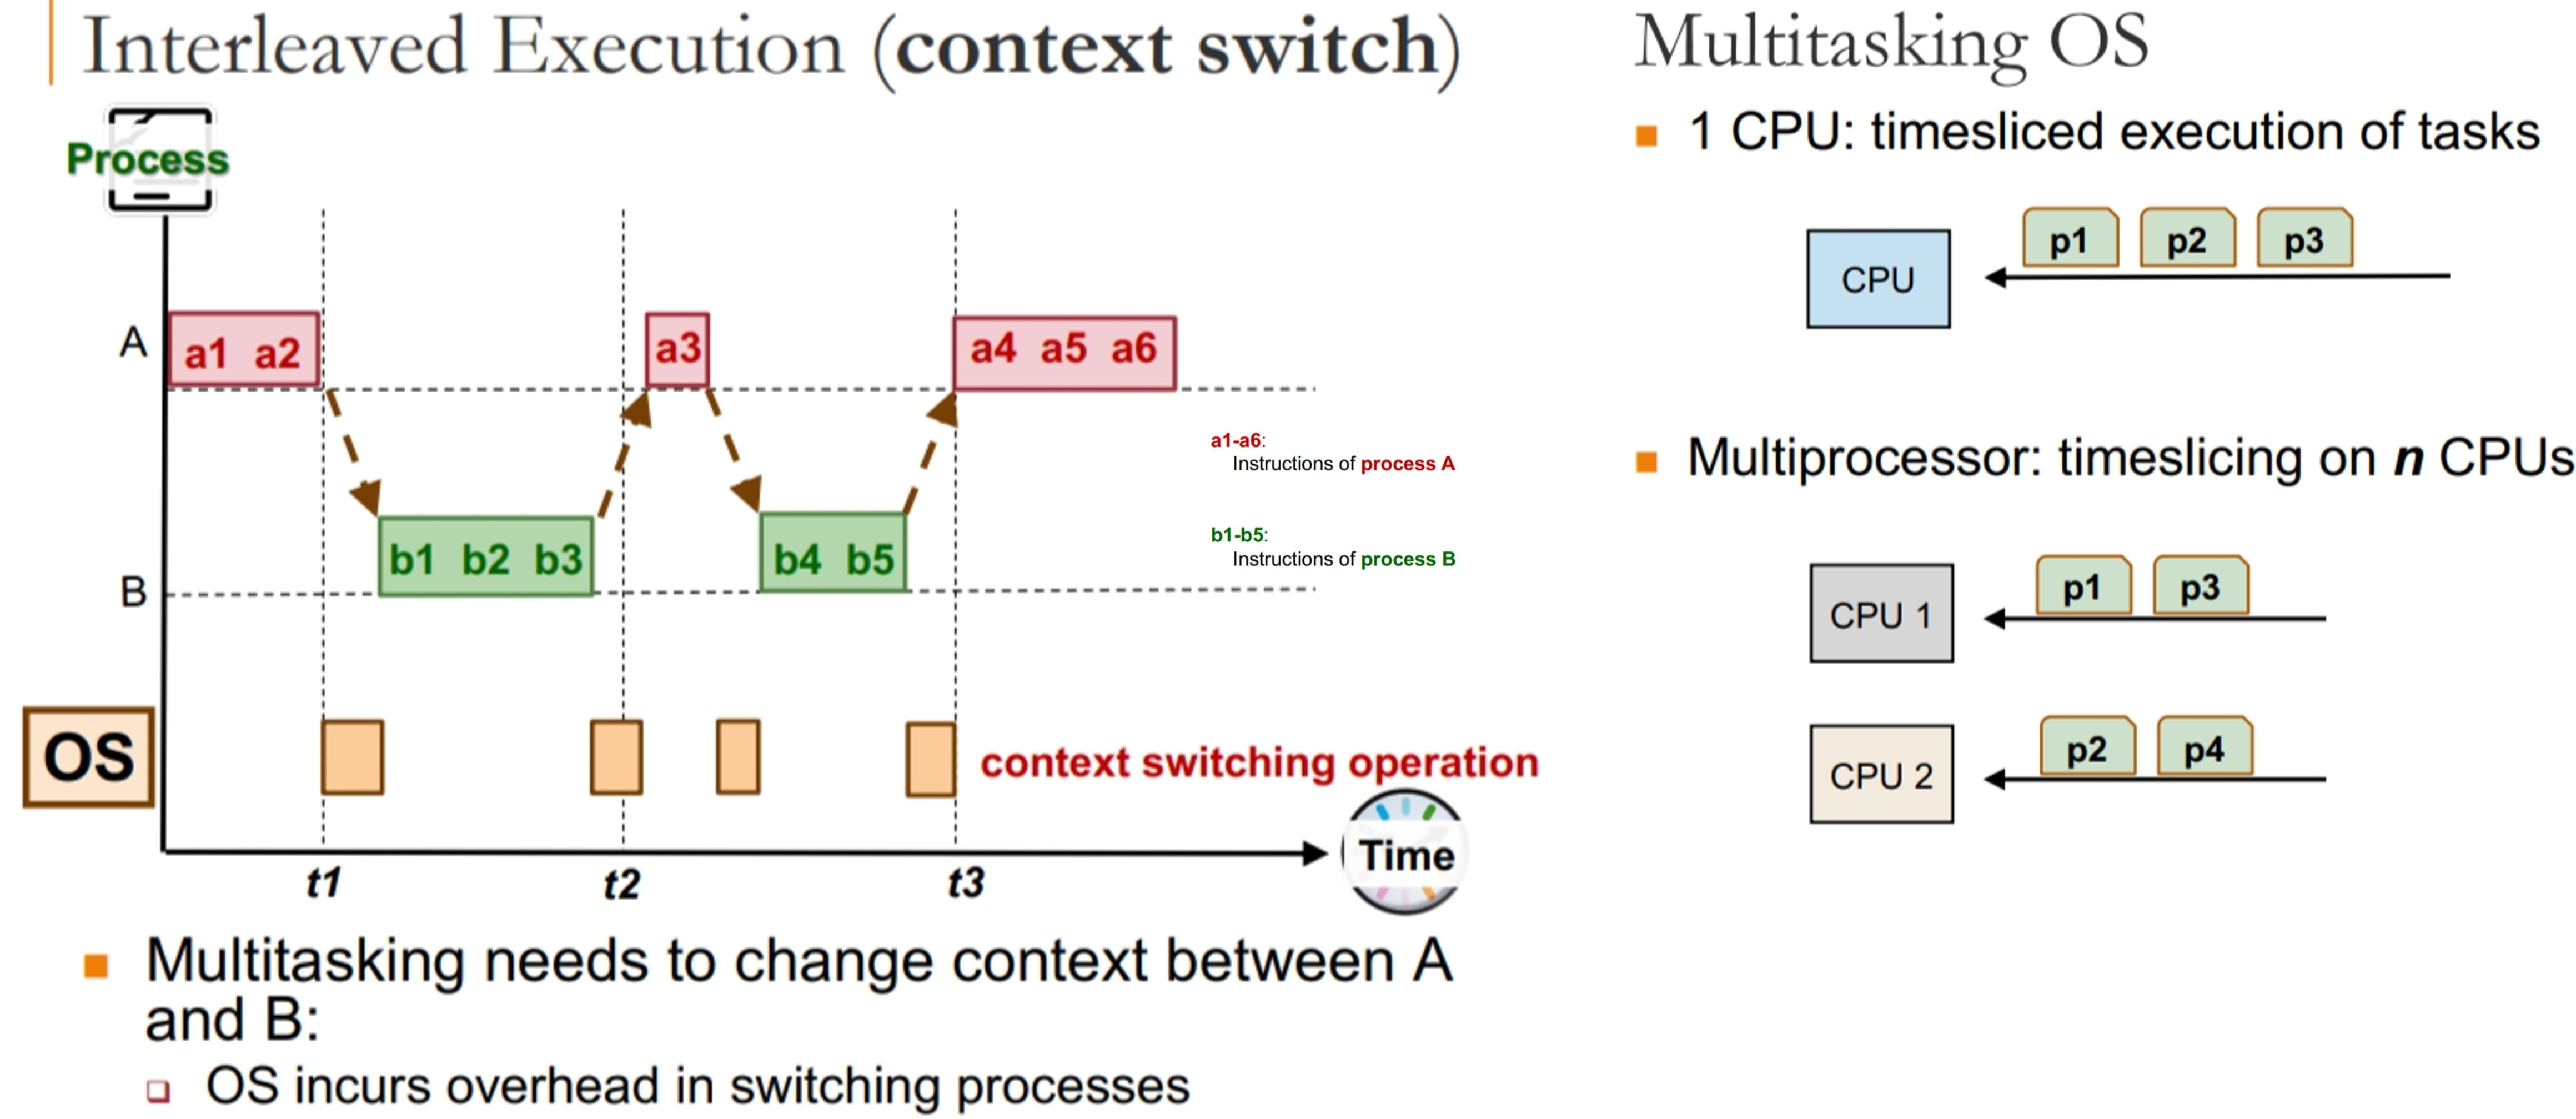
\includegraphics[width=1\linewidth]{timeslice}}
\begin{itemize}
\item \textbf{Scheduling a Process}: \\
1. Scheduler triggered (OS takes over) \\
2. If Context Switch needed, save context, place on blocked/ready queue. \\
3. Pick suitable process $P$ to run base on scheduling algo. \\
4. Setup context for $P$. \\
5. Let process $P$ run.
\end{itemize}

\null \null \null \null \null \null
\null \null \null \null \null \null
\null \null \null \null \null \null
\columnbreak

\section{Scheduling in Batch Systems}
\textbf{Environment}: No user interaction, non-preemptive scheduling predominant. \\
Scheduling algoritms generally easier to understand and implement, with variants and improvements for other type of system. \\
\textbf{Criteria}: Turnaround time (related to waiting time, time spent waiting for CPU). Throughput. CPU utilization.

\subsection{Batch Systems Scheduling Algorithms}
\subsection{FCFS: First-Come First-Served}
\begin{itemize}
\item Tasks stored on \textbf{FIFO queue based on arrival time}.
\item Pick first task in queue to run until done / blocked. Blocked task removed from FIFO queue, when ready, place at back of queue ("newly arrived").
\item \textbf{Evaluation}: \\
- \textit{No starvation}. (Every task eventually processed) \\
- \textit{Covoy Effect}. (CPU-Bound followed by IO-Bound tasks heavily inefficient.) Simple reordering can reduce average waiting time.
\end{itemize}

\subsection{SJF: Shortest Job First (Nonpreemptive)}
\begin{itemize}
\item Select task with \textbf{smallest total CPU time}.
\item Need to know total CPU time for task in advance. \\
- Possible to guess future CPU time by previous CPU-bound phases. 
\end{itemize}
\centerline{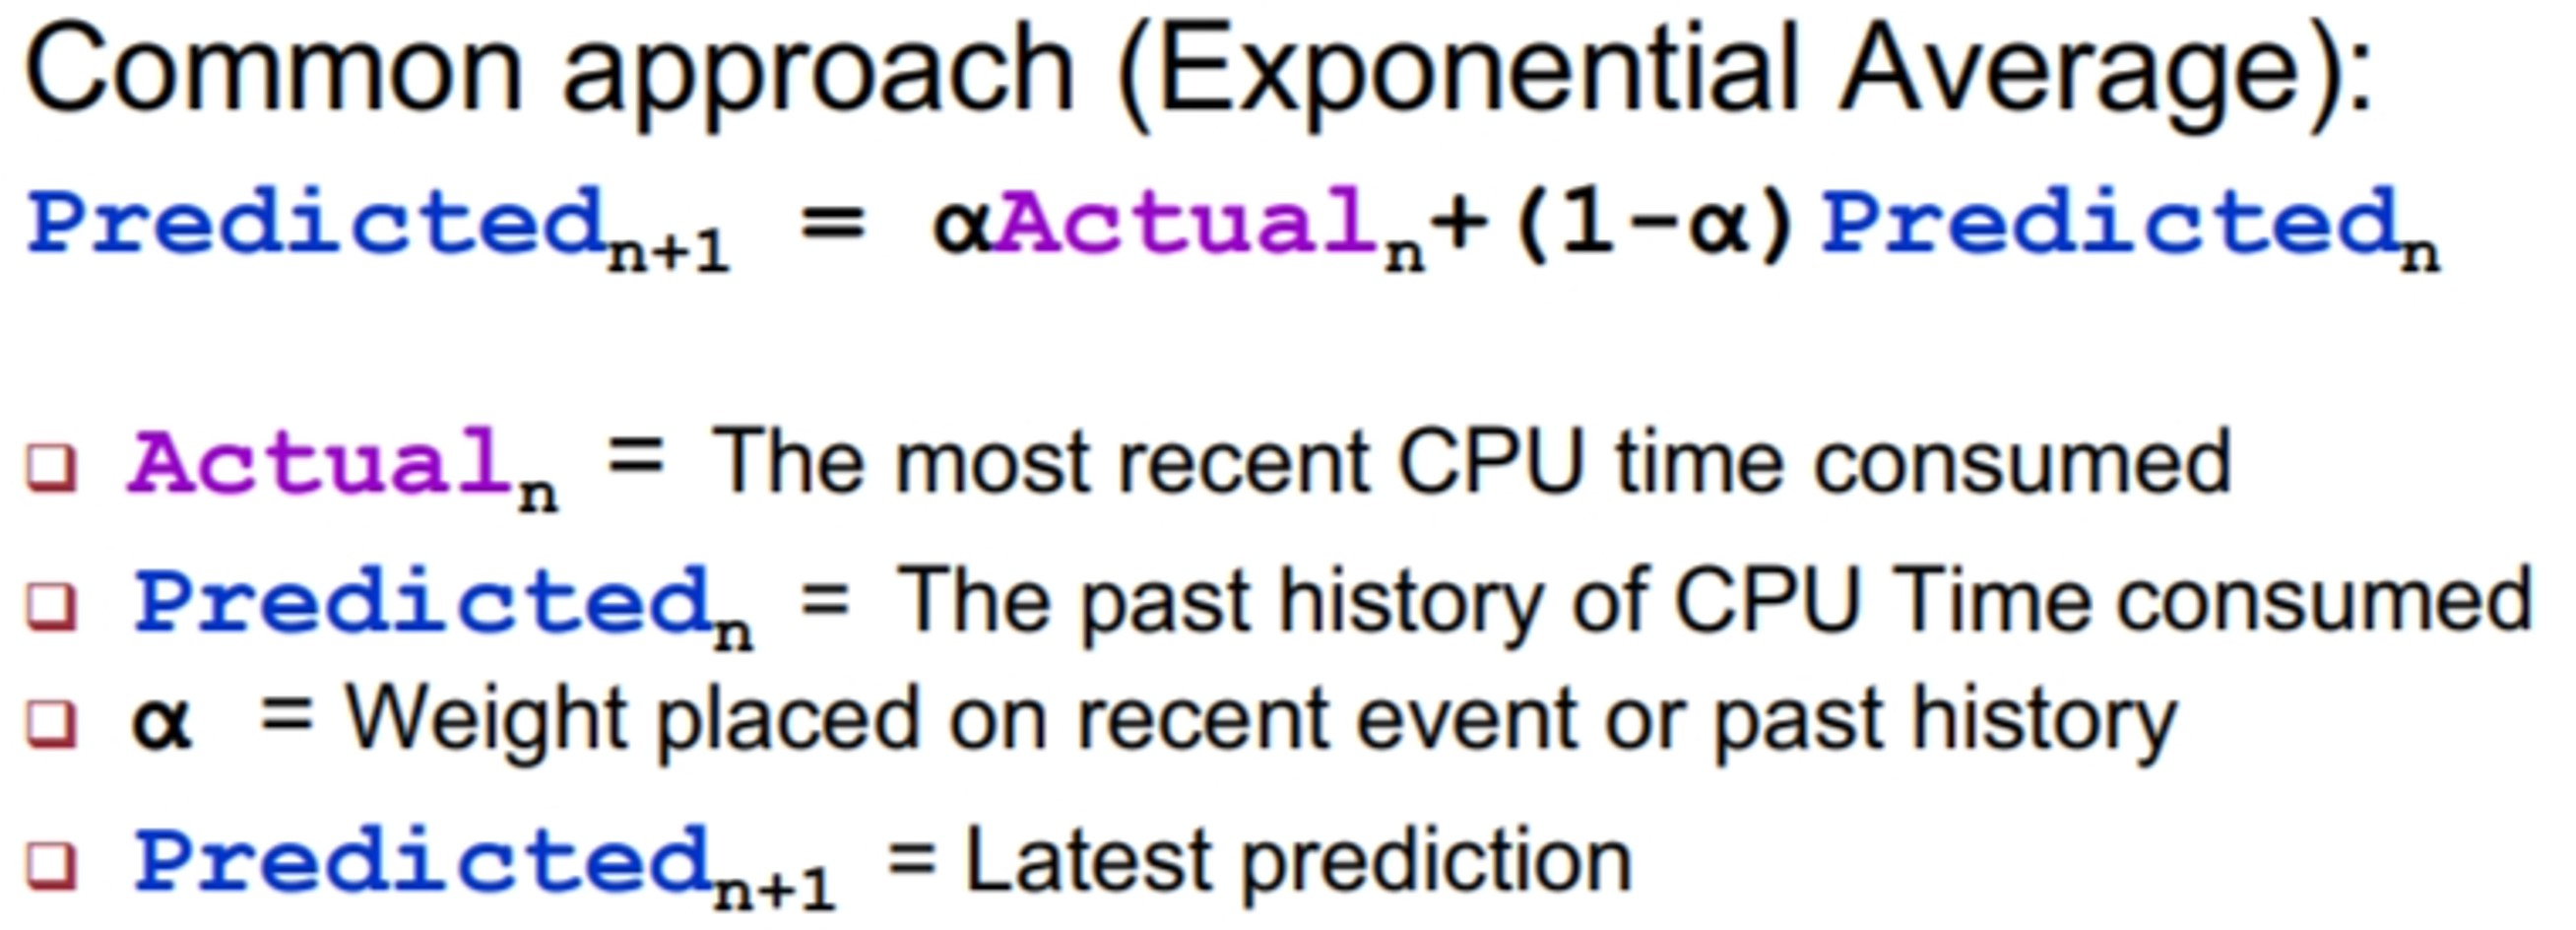
\includegraphics[width=0.6\linewidth]{exponentialAverage}}

\begin{itemize}
\item \textbf{Evaluation}: \\
- \textit{Starvation Possible} (Biased towards short jobs)
- \textit{Minimize average waiting time}.
- Optimal only when all jobs available simultaneously.
\end{itemize}

\subsection{SRT: Shortest Remaining Time Next (Preemptive)}
\begin{itemize}
\item \textbf{Preemptive ver of SJF}. \\
- Scheduler chooses process whose remaining run time is shortest.
\item When new job arrives, total time compared to current process' remaining (or expected) time.
\end{itemize}

\subsection{Batch System Scheduling Examples}
\centerline{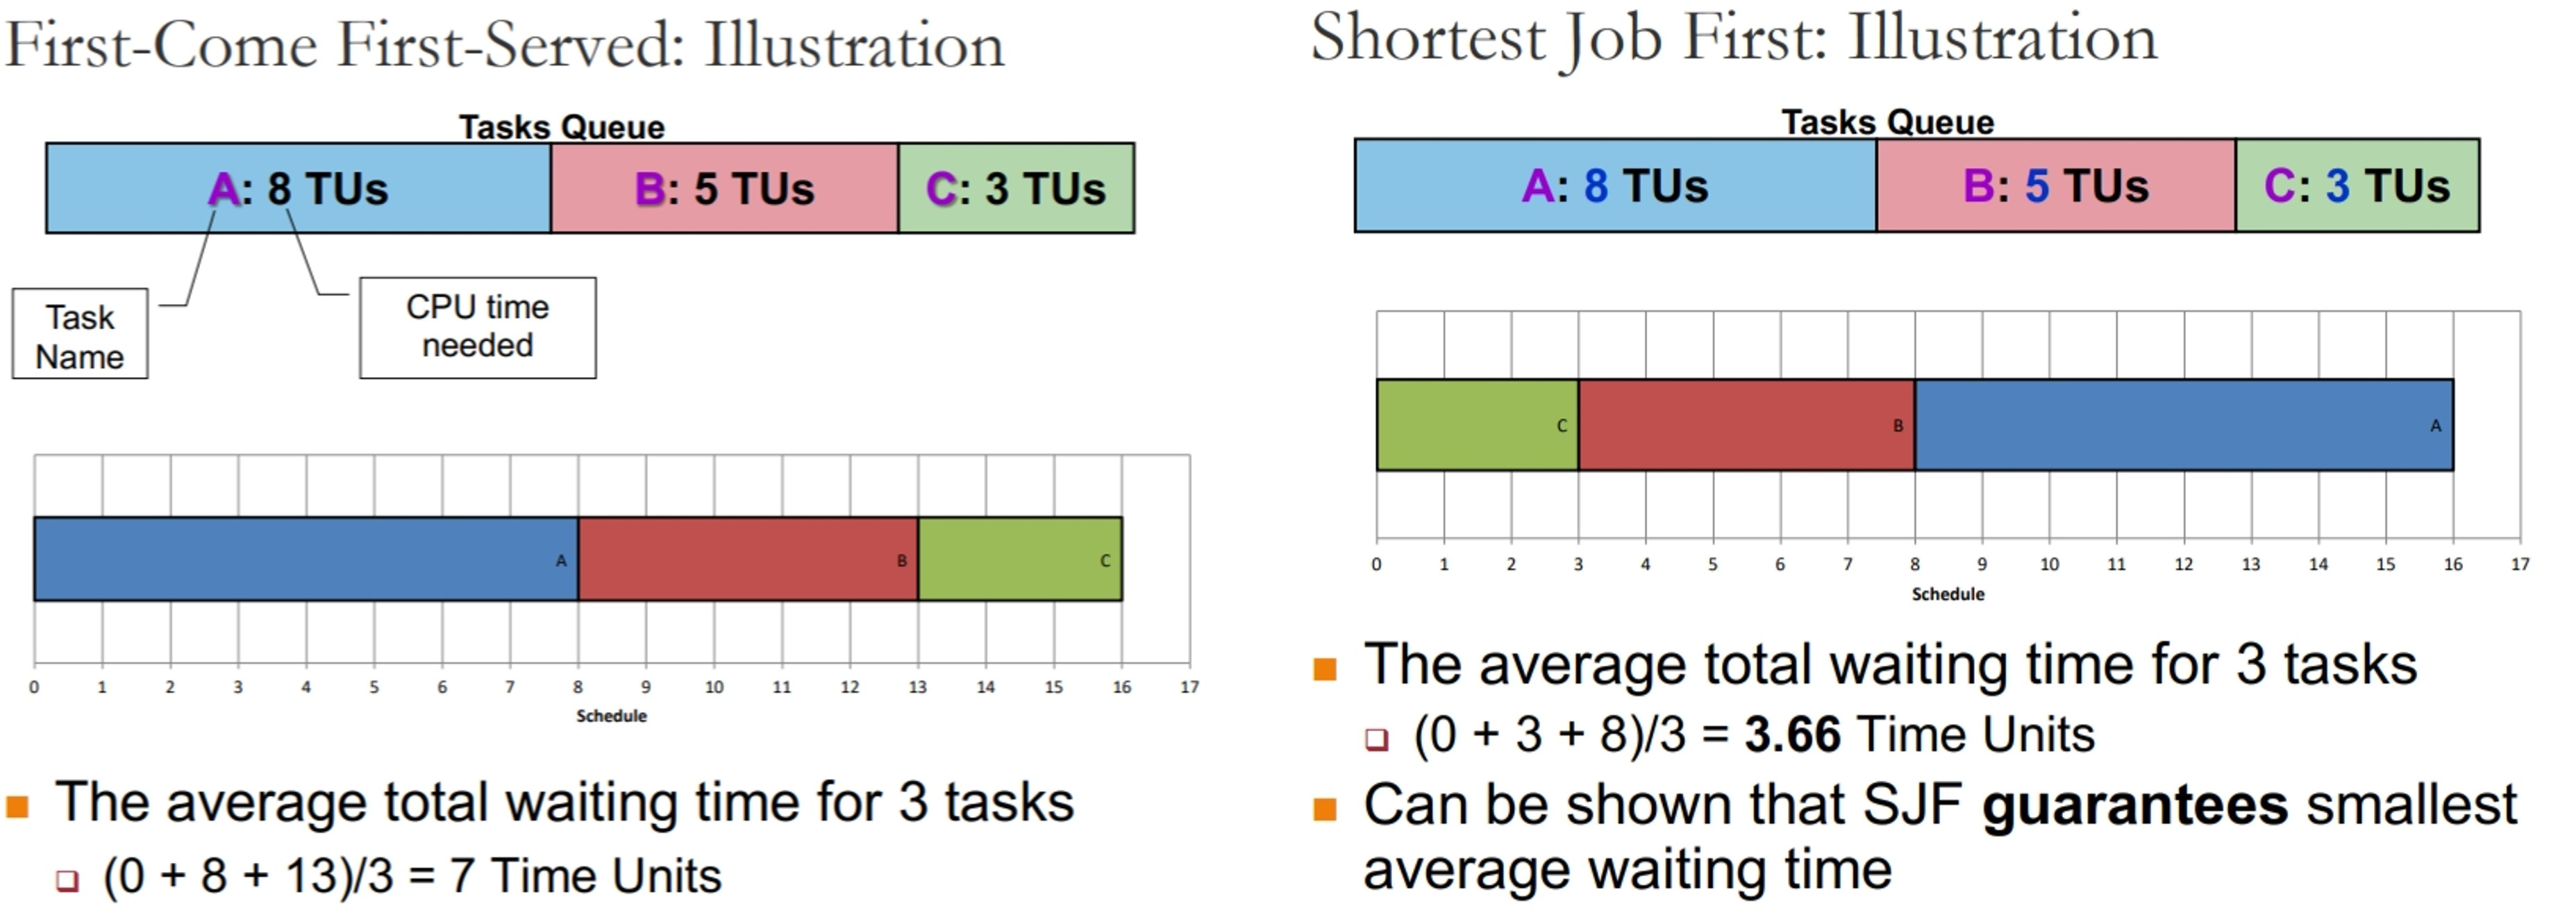
\includegraphics[width=1\linewidth]{batchScheduling}}

\null
\columnbreak

\section{Scheduling in Interactive Systems}
\textbf{Criteria}: Response time (time btwn request \& response). Predictability (Less variation in response time). \\
\textbf{Environment}: User interaction. Preemptive scheduling used to ensure good response time. Scheduler needs to run periodically. \\
\textbf{Ensuring Periodic Scheduler}: Use timer \textbf{interrupts} (based on hardware clock). OS ensures timer interrupt cannot be intercepted by any other program. Interrupt handle \textbf{invokes scheduler}.
\begin{itemize}
\item \textbf{ITI: Interval of Timer Interrupt}: Timing Interval that interrupt happens, and OS scheduler triggered. Typical values (1ms - 10ms).
\item \textbf{Time Quantum}: Execution duration given to each process, constant / variable. Must be multiples of ITI. Typical values (5ms - 100ms).
\end{itemize}
\centerline{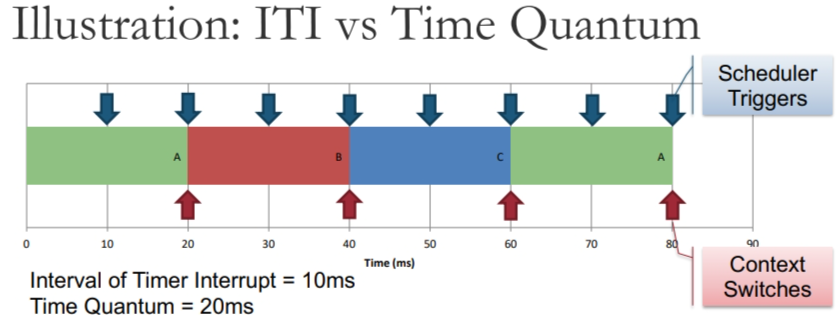
\includegraphics[width=0.8\linewidth]{ITI}}

\subsection{Interactive Systems Scheduling Algorithms}
\subsection{RR: Round Robin}
\begin{itemize}
\item Preemptive ver. of FCFS.
\item \textbf{Tasks stored in FIFO queue}. Each process assigned time quantum.
\item If task still running at end of quantum / blocked / gives up CPU voluntarily, CPU preempted, given to another process. 
\item Task placed at end of queue to wait for another turn.
\item \textbf{Response time guarantee}: $n$ tasks, $q$ quantum. \\
Time before task gets CPU bounded by $(n-1)q$.
\item \textbf{Evaluation}: \\
- Too short quantum $=$ many process switches, lower CPU efficiency \\
- Too long quantum causes poor response to short interactive requests.
\end{itemize}

\subsection{Priority Scheduling: Priority Based}
\begin{itemize}
\item Each process assigned a priority, runnable process with highest priority p allowed to run. \\
- \textbf{Preemptive ver.}: Higher p. process can preempt running low p. process. \\
- \textbf{Non-preemptive ver.}: Late high p. process wait for next scheduling.

\item \textbf{Evaluation}: \\
- \textbf{Possible Starvation}: High p. process may hog CPU. \\
To prevent this, scheduler may \textbf{decrease priority} of currently running process at each clock tick (clock interrupt). Or, give some max time quantum, when used up, allow next in line to run. \\
- \textbf{Priority Inversion}: When lower priority task preempts higher priority task. (If lower priority task locks some resource, e.g. file, gets switched, higher priority task cannot run)
\end{itemize}

\columnbreak

\subsection{MLFQ: Multi-Level Feedback Queue}
\begin{itemize}
\item More efficient to give CPU-bound process large quantum once in a while, rather than small quanta frequently to reduce swapping. Also, giving all processes large quantum means poor response time. \\
Hence, solution to set \textbf{multiple priority queues}.
\item As (CPU-bound) process sinks deeper into priority queues, run less frequently, saving CPU for short, interactive processes.
\item Hence, \textbf{adaptively learn process behavior}, minimize both: \\
- Min. Response time for IO bound processes \\
- Min. Turnaround time for CPU bound processes.
\item \textbf{MLFQ Rules}: \\
- \textbf{Basic Rule}: Higher priority process runs. If same p, run in RR. \\
- \textbf{Priority Setting}: New job given highest priority. If job fully utilize time slice, priority reduced. If job gives up / blocks before time slice finished, priority retained.
\item \textbf{Evaluation}:
- \textbf{Can be gamed}: User typing carriage returns at random every few seconds doing wonders for his response time.
\end{itemize}


\subsection{Lottery Scheduling}
\begin{itemize}
\item Give processes lottery tickets for system resources. When scheduling, chose ticket at random.
\item "All processes equal, some processes more equal." More important processes given extra tickets.
\item \textbf{Evaluation}: \\
- \textit{Responsive}: New process can participate in next lottery. \\
- \textit{Good Control}: Each process can distribute to child processes proportionally w.r.t to need. \\
\end{itemize}

\subsection{Interactive System Scheduling Examples}
\centerline{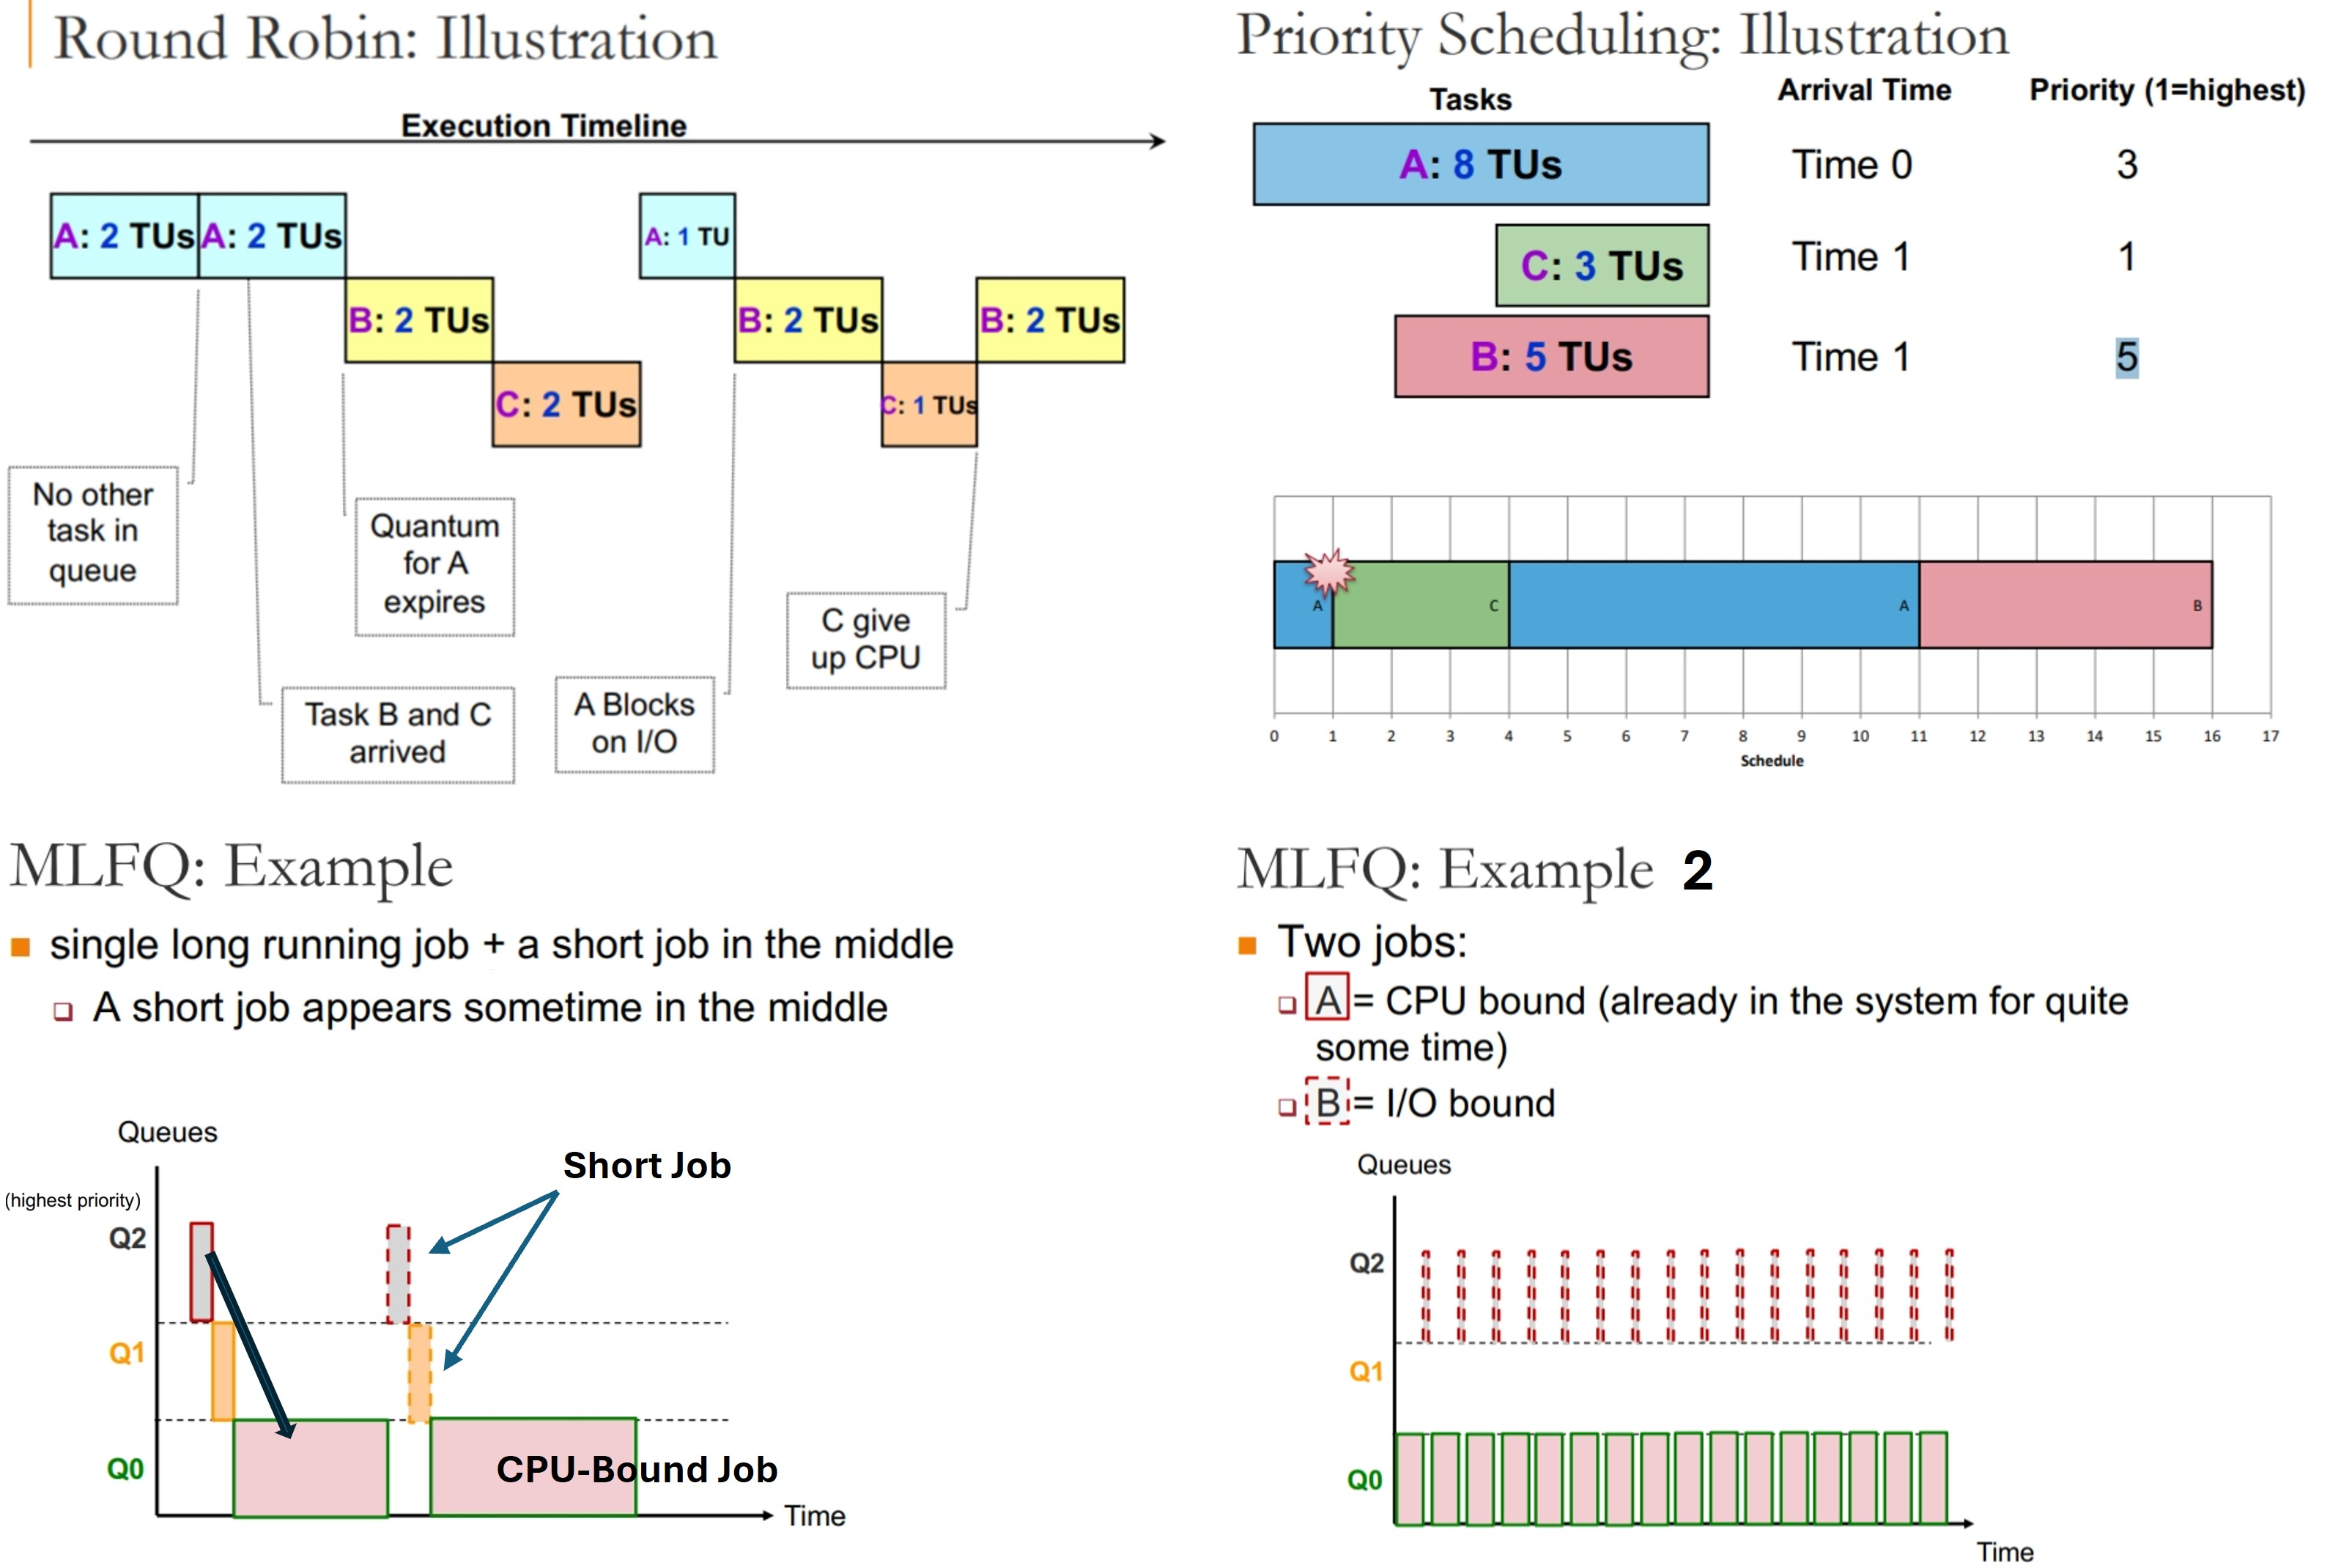
\includegraphics[width=1\linewidth]{interactiveScheduling}}


\subsubsection{Others}
\begin{itemize}
\item \textbf{Shortest Process Next}: Estimate (using calculated aging).
\item \textbf{Guaranteed / Fair-Share Scheduling}: Track CPU usage, run accordingly. Each user gets agreed allocation of CPU.
\end{itemize}



\columnbreak

\section{4. Threads}
In trad. OS, each process has an address space and single thread of control. Desirable instead to have multiple threads of control in the same address space running in quasi-prallel, as though (almost) separate processes (except for shared address space).

\subsubsection{Motivation for Thread}
\begin{itemize}
\item \textbf{Process is Expensive}: Process creation under \code{fork()} model duplicate memory space, most of process context.
\item Context switch also requires overhead, save/restore process info.
\item \textbf{Communication}: Hard for independent processes to communicate with each other. Independent memory space, no shared variable, requires IPC.
\item \textbf{Thread}: "quick hack" into popular mechanism. 
\item \textbf{Basic Idea}: Traditional process only single thread of control. (Only one instruction executing at a time). 
\item Add more threads (of control) to same program, multiply parts of programs executing at same time conceptually.
\end{itemize}

\subsection{Process and Thread}
\begin{itemize}
\item \textbf{Multi-threaded Process}: Single process can have multiple threads.
\item Threads in same process share same: \textit{Memory Context} (text, data heap), \textit{OS Context} (Process id, files etc.)
\item \textbf{Unique info per thread}: Id (thread id), Registers (GPR and special), "Stack".
\item \textbf{Process Context Switch vs. Thread Switch}: \\
- \textit{Process Context Switch}: Switch OS, Hardware, Memory Context.\\
- \textit{Thread Switch (same process)}: Just hardware context (registers, stack). \\
- Thread is \textbf{lightweight process}.
\end{itemize}
\centerline{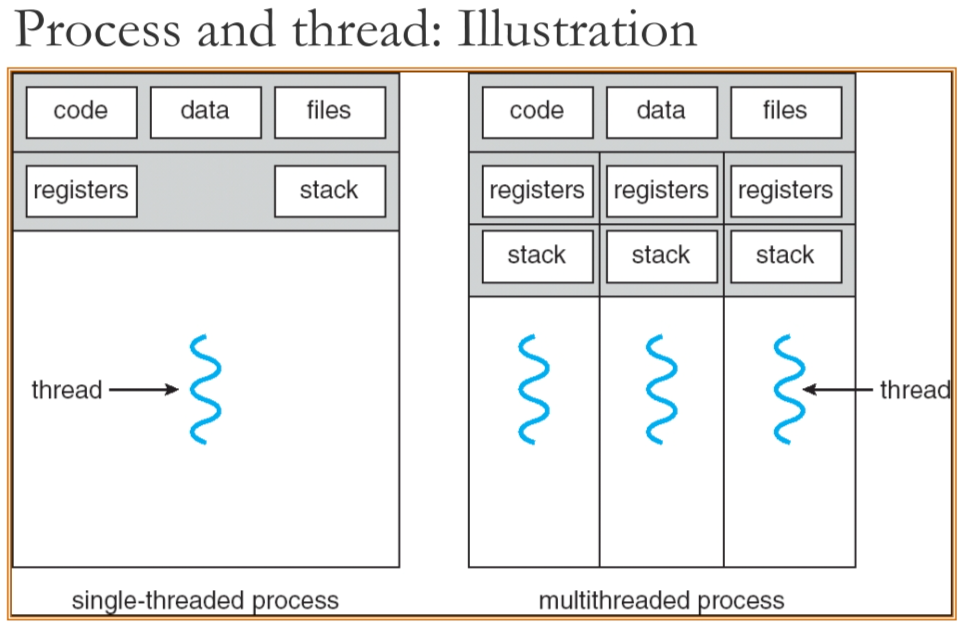
\includegraphics[width=0.5\linewidth]{ProcessThread}}

\subsubsection{Threads: Benefits}
\begin{itemize}
\item \textbf{Resource Sharing}: Ability for parallel entities to share address space and all of data. No need add. mechanism for passing info.
\item \textbf{Economy}: Threads are lighter weight than process, faster to create and destroy. Less resources to manage.
\item \textbf{Responsiveness}: No performance gain when all CPU bound, but when substantial computing and substantial I/O, threads allows activities to overlap, speeding up application.
\item \textbf{Scalability}: Multithreaded program can take advantage of multiple CPUs.
\end{itemize}

\subsubsection{Threads: Problems}
\begin{itemize}
\item \textbf{System Call Concurrency}:  Parallel execution of multiple threads: parallel system call possible. Need to guarantee correctness and determine correct behavior.
\item \textbf{Process Behavior (OS dependent)}: Impact on process operations, (e.g. If one thread executes exec() / exit(), what about other threads / whole process).
\end{itemize}

\subsection{Thread Models (ways to support threads)}
\begin{itemize}
\item \textbf{User Thread}: Thread implemented as a \textbf{user library}. (Runtime system (in the process) will handle thread related operation.)
\item Kernel not aware of threads in process.
\item \textbf{Kernel Thread}: Thread implemented in the OS. Operation handled as system calls. 
\item Kernel thread-level scheduling possible, where kernel schedule by threads instead of by process.
\item Kernel may make use of threads for own execution.
\item \textbf{Threads on Modern Processor}: Threads started as software mechanism, now exists hardware support on modern processors (multiple register sets on same core, \textit{simultaneous multi-threading (SMT)}, "Hyperthreading" on Intel).
\end{itemize}

\subsubsection{User Thread}
\begin{itemize}
\item \textbf{Advantages}: Can have any multithreaded program on any OS, thread operations are just library calls, generally more configurable and flexible (e.g. customized thread scheduling policy.)
\item \textbf{Disadvantages}: OS not aware of threads, scheduling is performed at process level. (One thread blocked, process blocked, all threads blocked). Cannot exploit multiple CPUs.
\end{itemize}

\subsubsection{Kernel Thread}
\begin{itemize}
\item \textbf{Advantages}: Kernel can schedule on thread levels: $>$ 1 thread in same process can run simultaneouly on multiple CPUs.
\item \textbf{Disadvantages}: Thread operations now system calls, slower and more resource intensive. Generally less flexible, used by all multithreaded programs, so too many / few features, overkill / not flexible enough for different programs.
\end{itemize}
\centerline{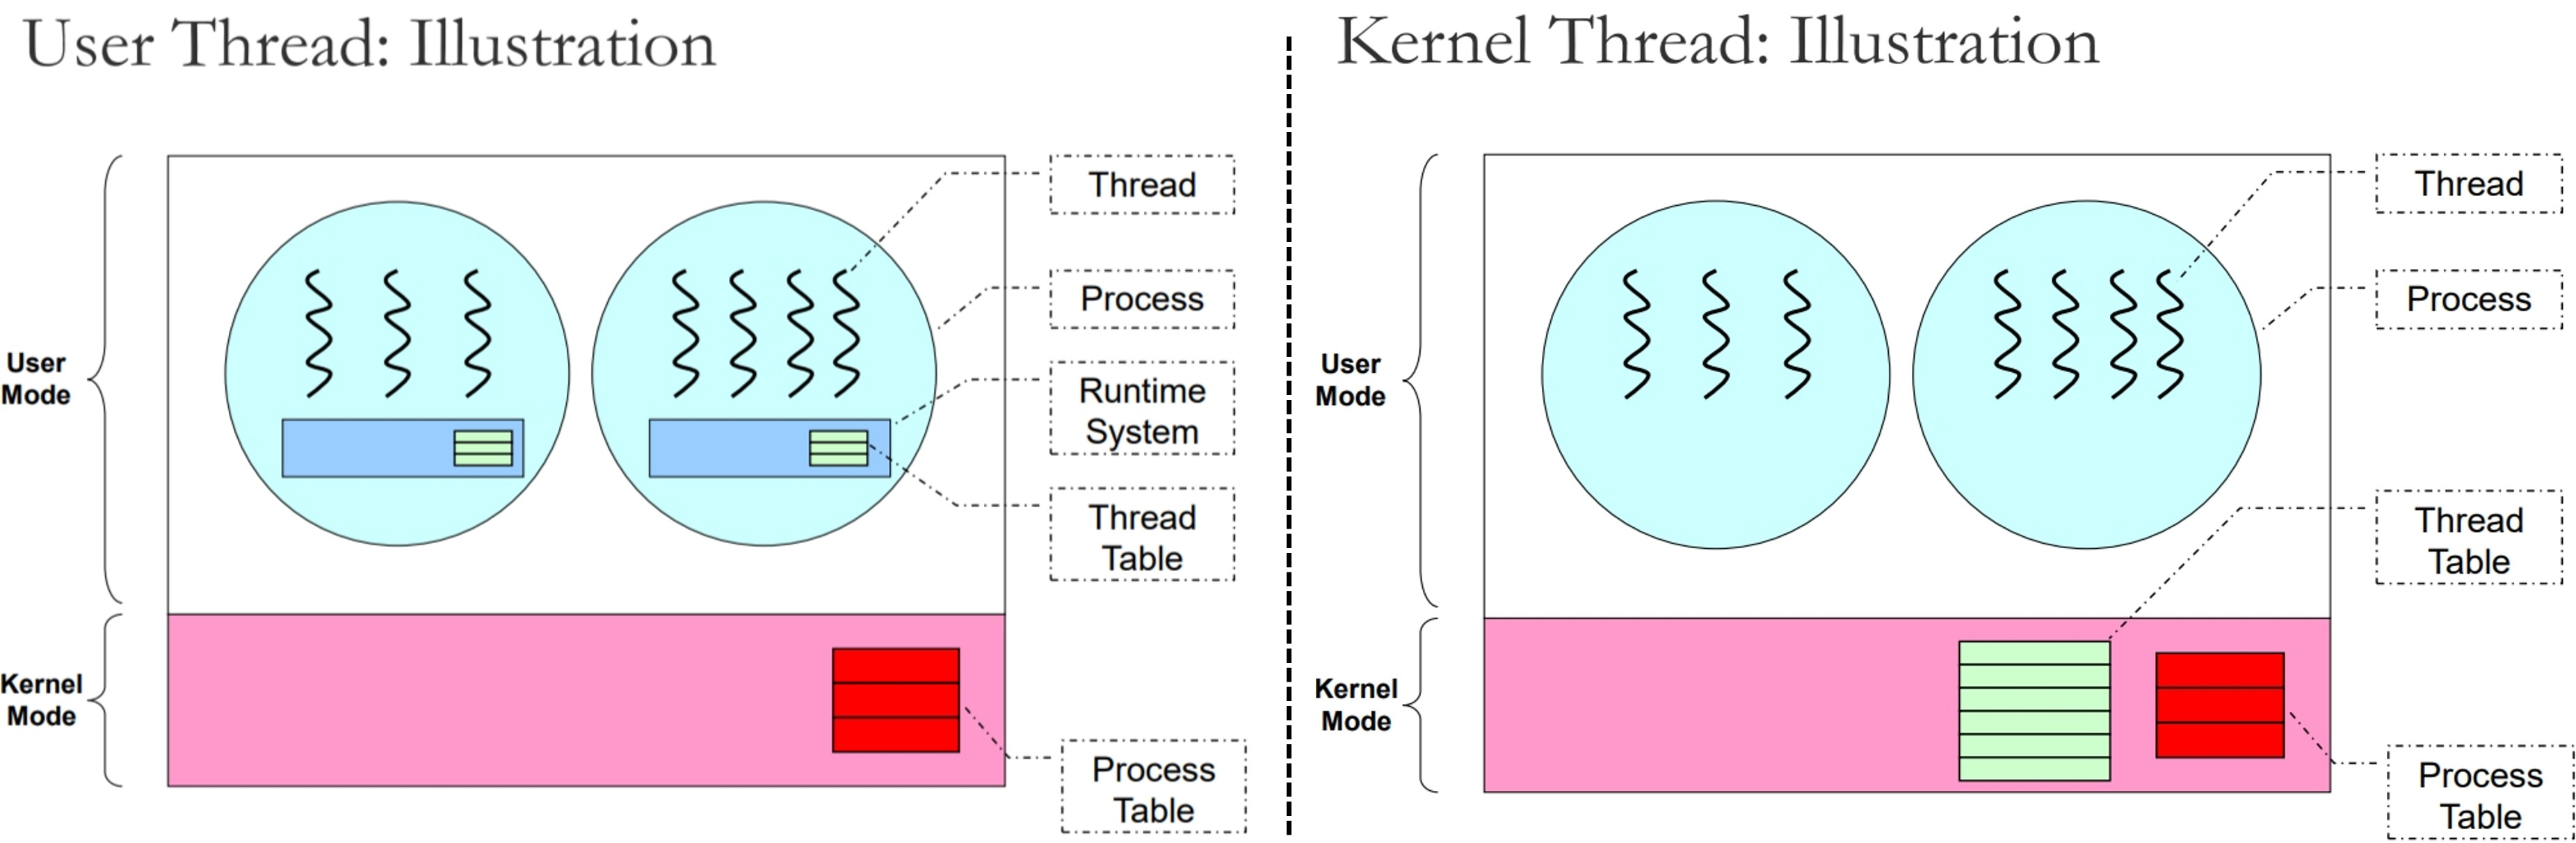
\includegraphics[width=1\linewidth]{UserKernelThread}}

\subsection{Hybrid Thread Model}
\begin{itemize}
\item Have both Kernel and User threads, where OS schedule on kernel threads only, and user thread binds to a kernel thread.
\item Offers flexibility, limit concurrency of any process / user.
\end{itemize}
\centerline{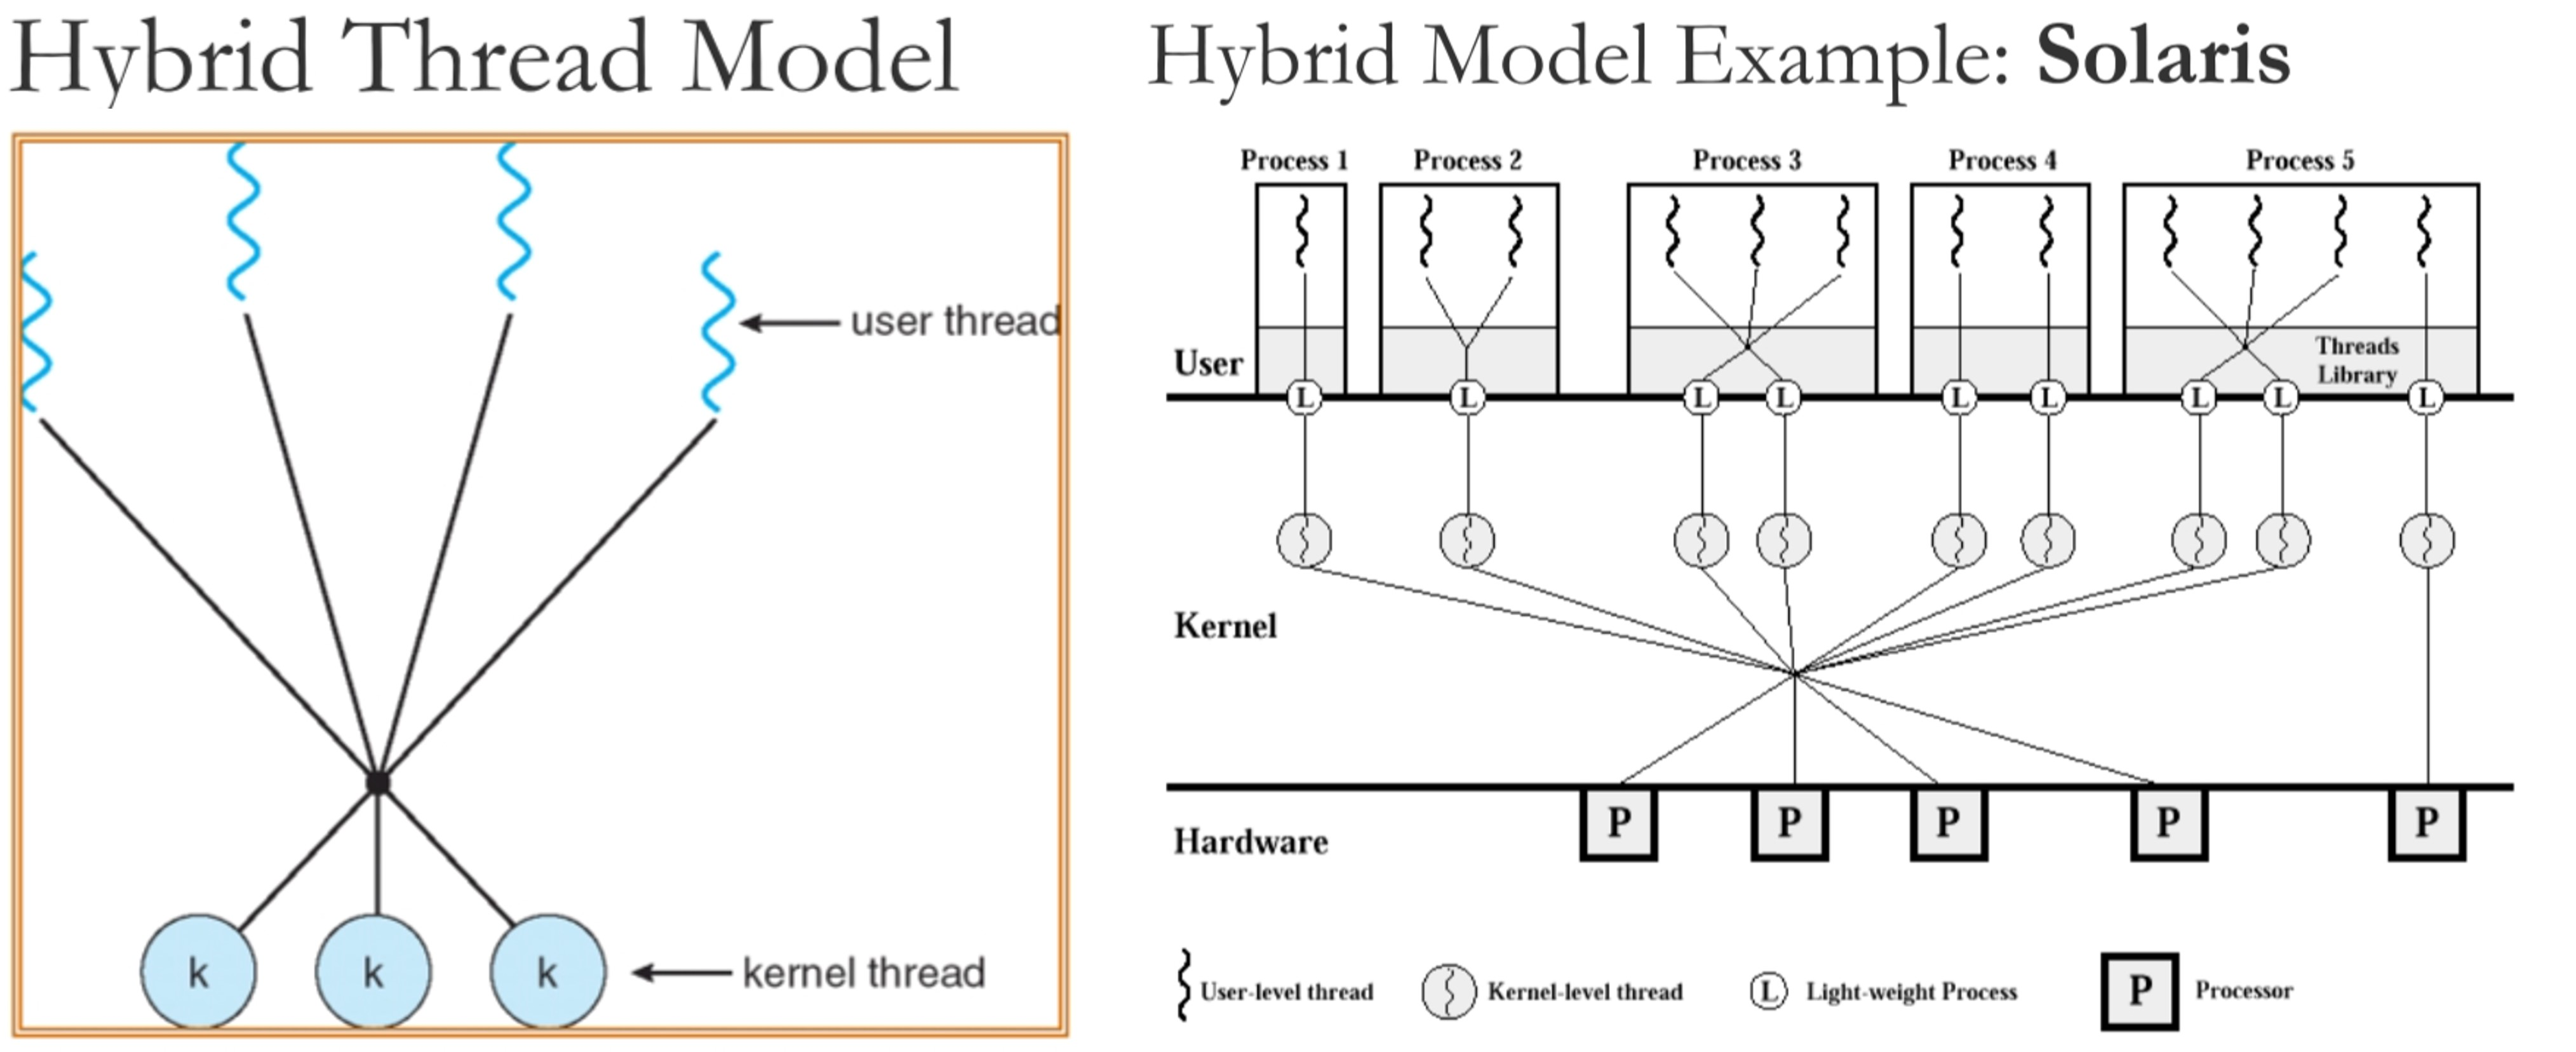
\includegraphics[width=1\linewidth]{hybridThreadModel}}

\section{POSIX Threads}
IEEE defined standards (1003.1c) for threads, called \textit{Pthreads}, most UNIX systems support it. Defines over 60 function calls.

\subsection{Pthread}
\begin{itemize}
\item \textbf{POSIX}: Portable Operating System Interface. (family of standards)
\item Defines the API as well as the behavior, but not implementation.
\item pthread can be implemented as user / kernel thread.
\end{itemize}

\centerline{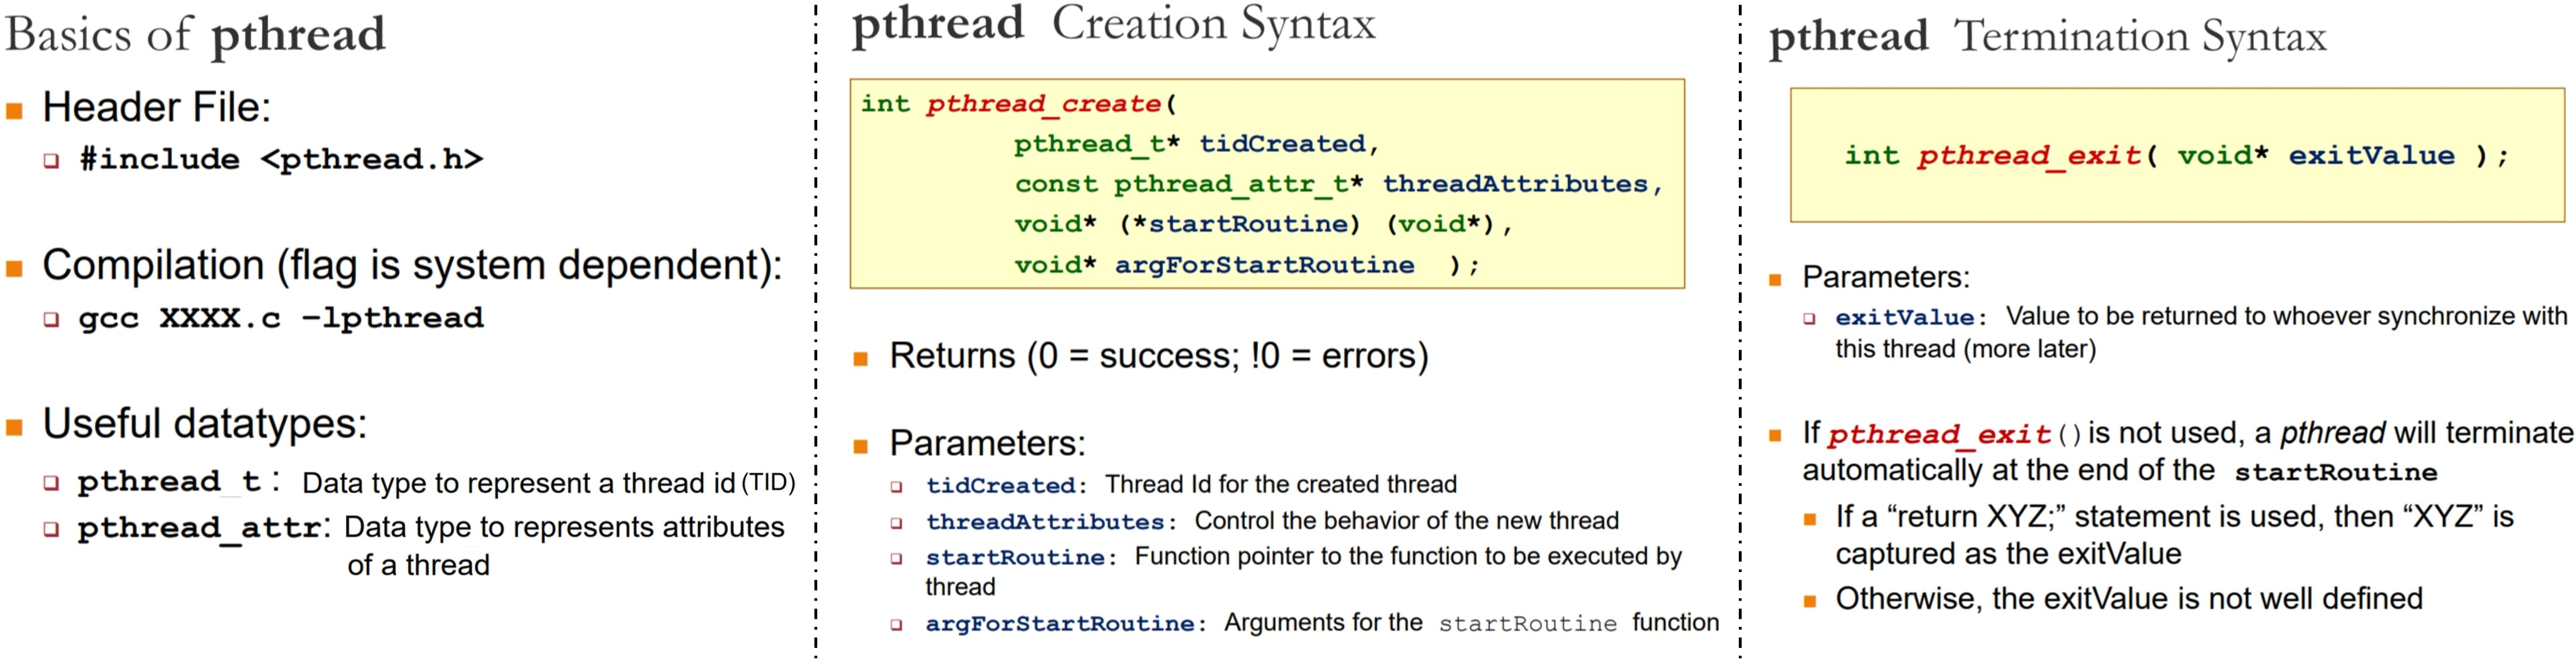
\includegraphics[width=1\linewidth]{pthreadBasics}}
\medskip
\centerline{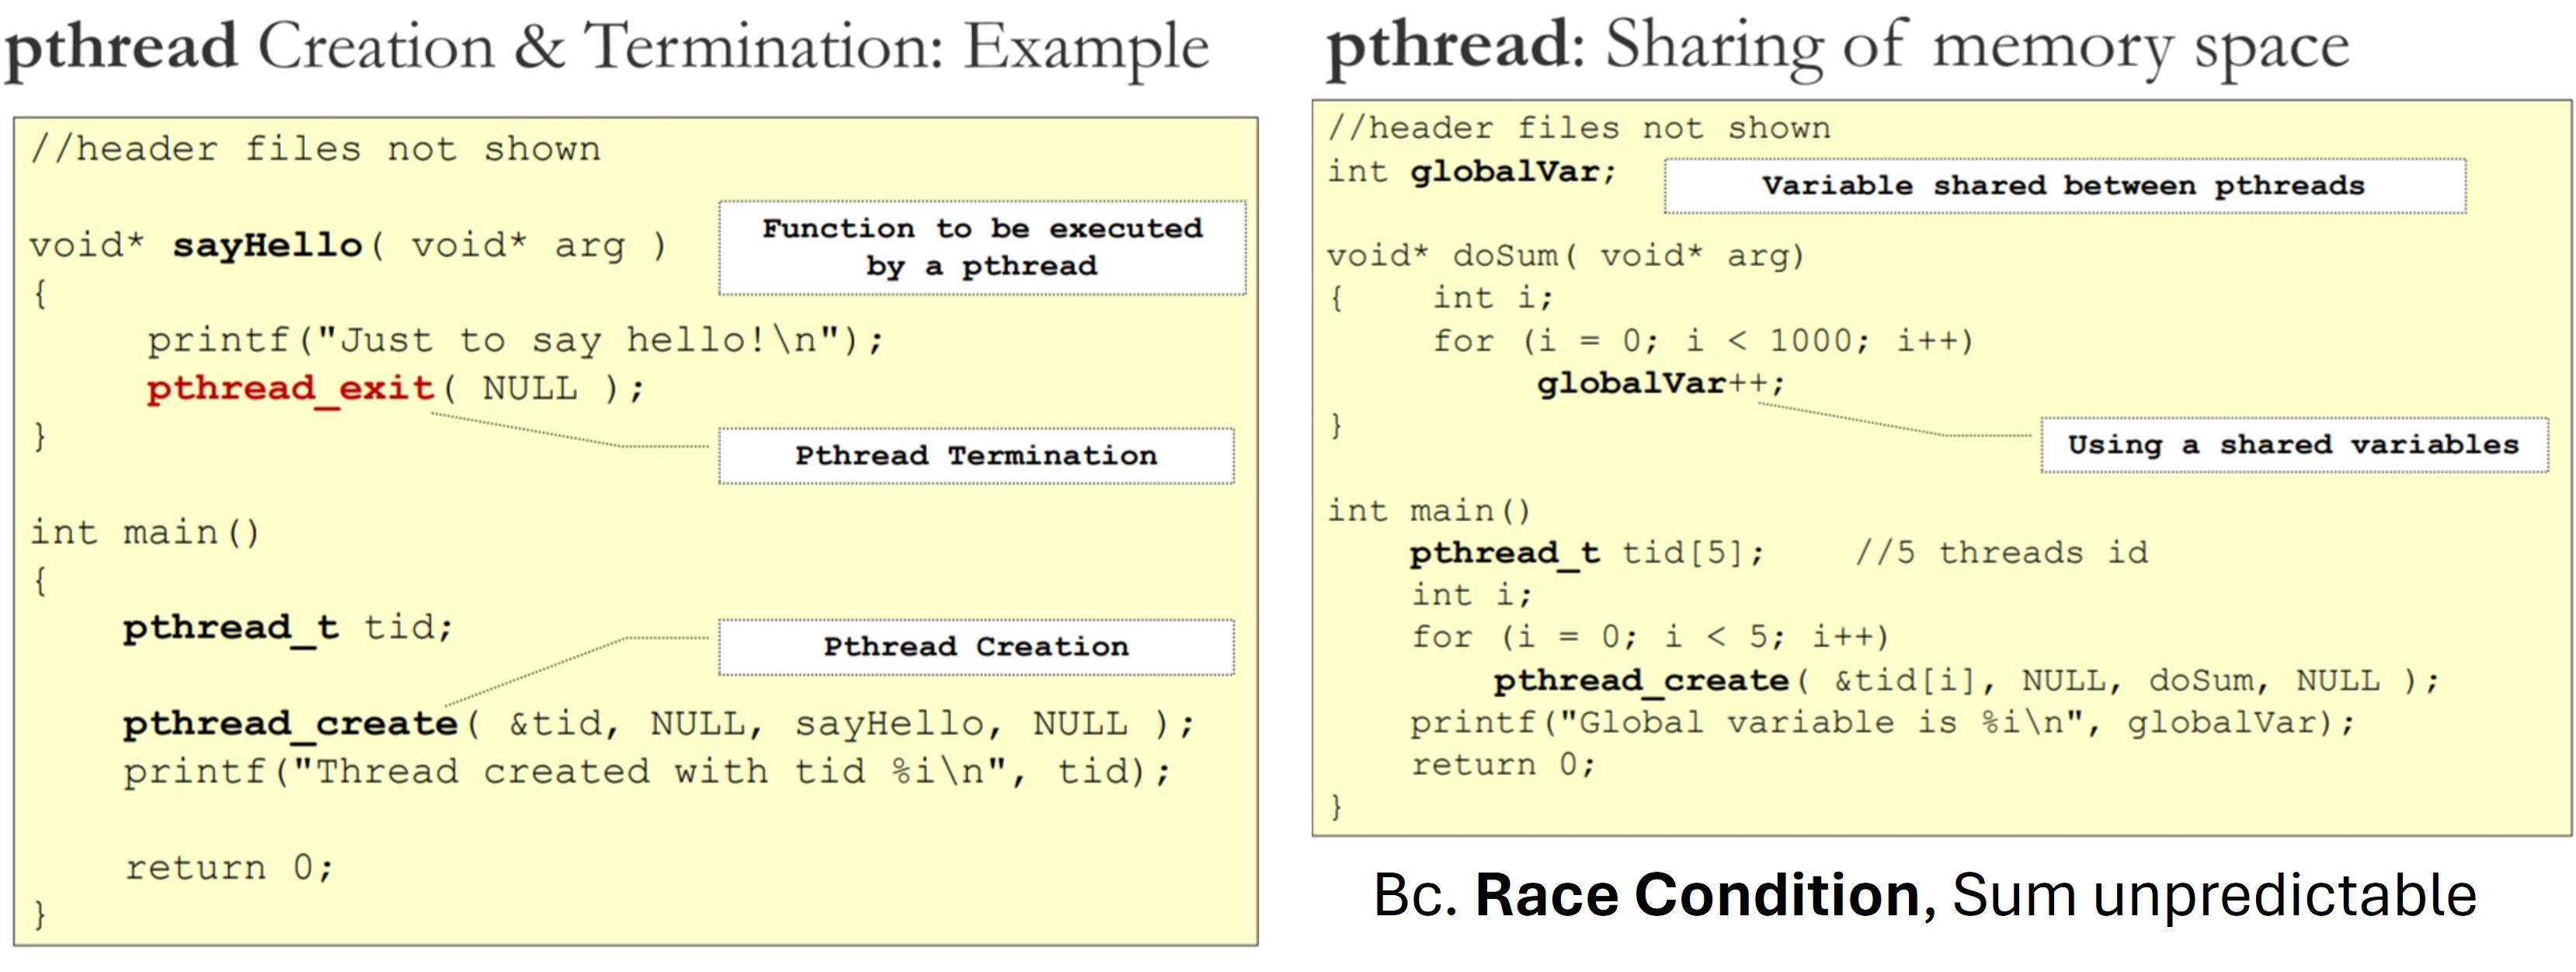
\includegraphics[width=1\linewidth]{pthreadExample}}

\begin{lstlisting} [linewidth = 1.0 \linewidth],
#include <stdio.h>
#include <pthread.h>
int globalVar;

void* doSum( void* arg){ 
    int i;
    for (i = 0; i < 1000; i++) {
        globalVar++; }
}


int main() {
    pthread_t tid[5]; //5 threads id
    int i;

    for (i = 0; i < 5; i++) {
        pthread_create( &tid[i], NULL, doSum, NULL ); }

    //Wait for all threads to finish
    for (i = 0; i < 5; i++) {
        pthread_join( tid[i], NULL ); }

    printf("Global variable is %i\n", globalVar);
    return 0;
}
\end{lstlisting}

\centerline{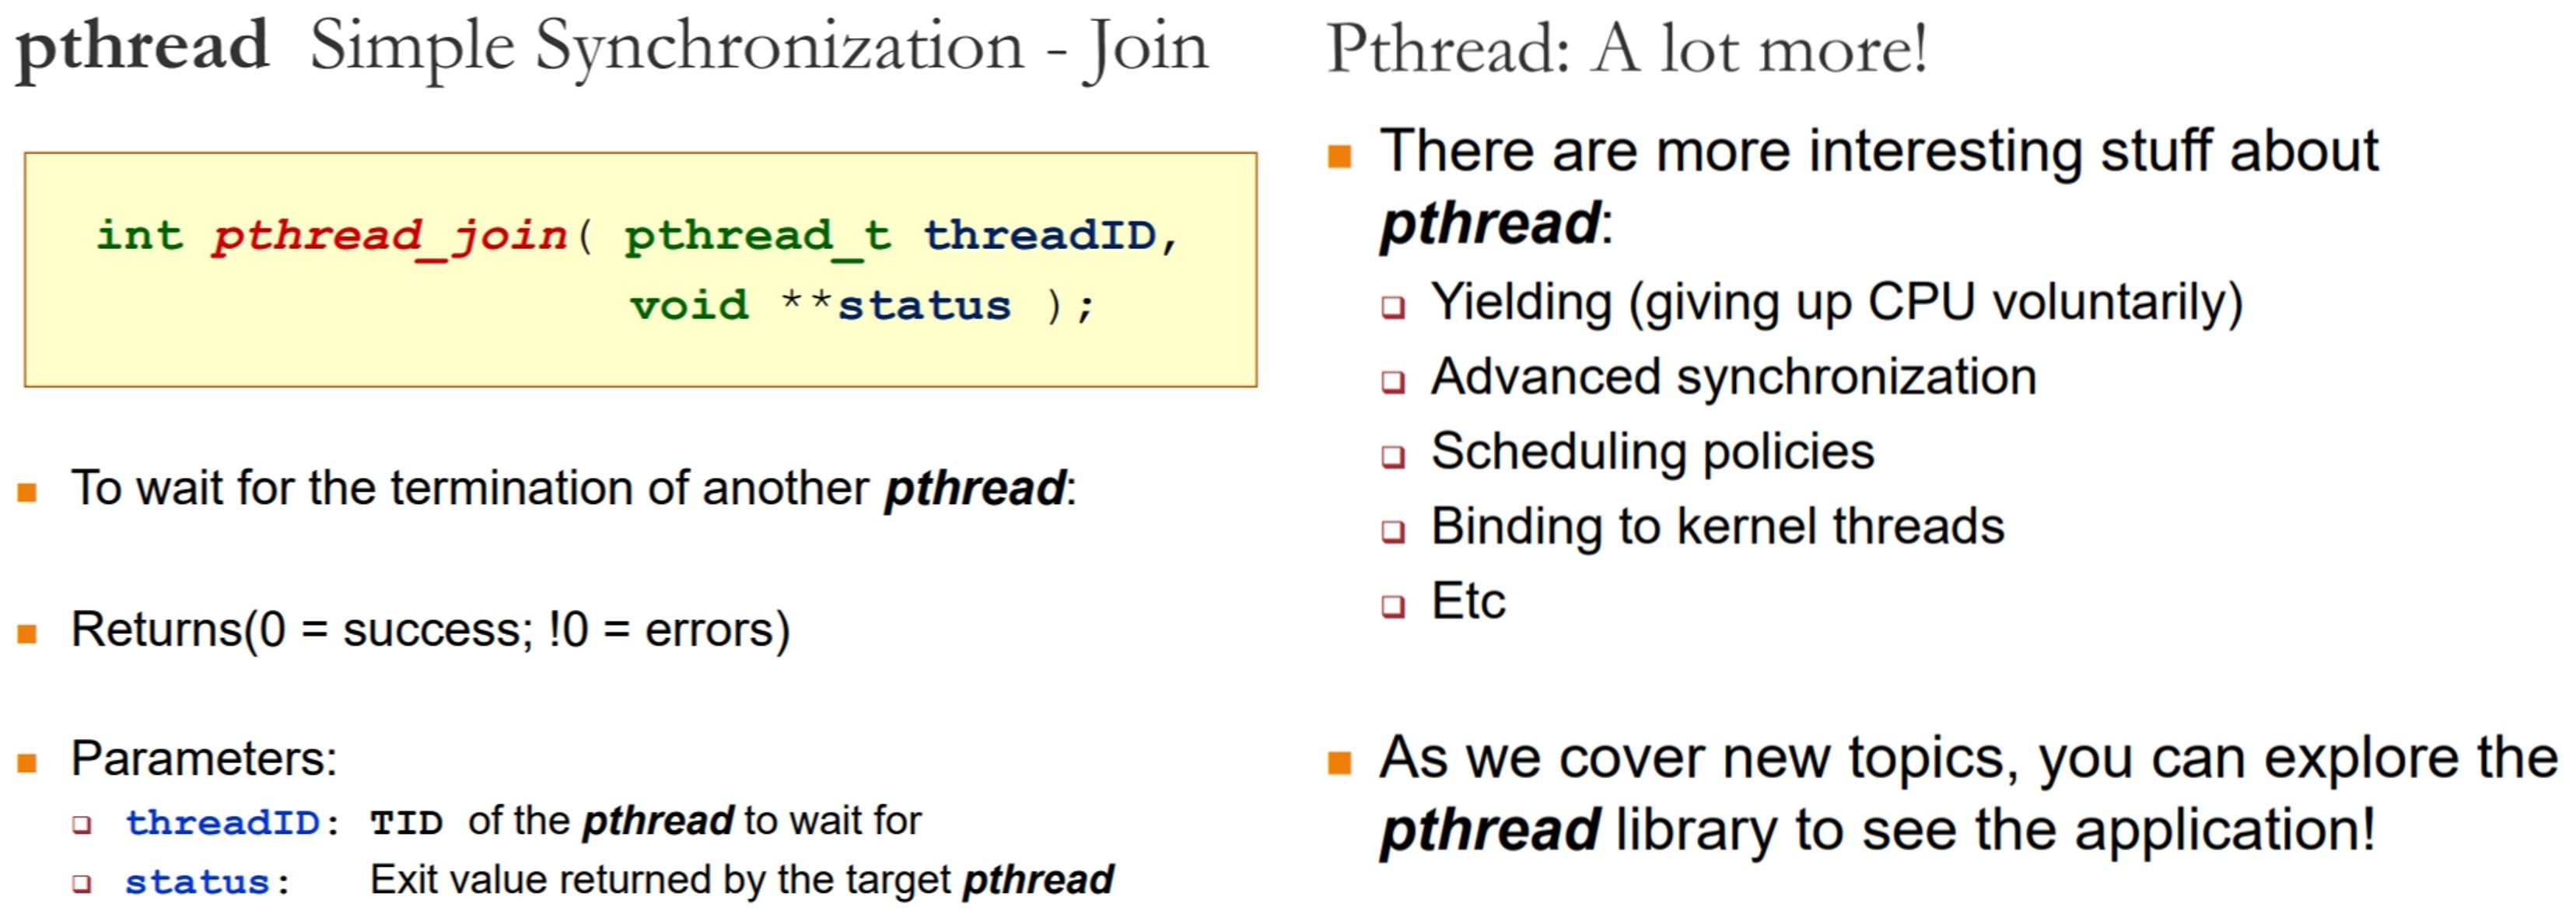
\includegraphics[width=1\linewidth]{pthreadSync}}

\columnbreak

\subsubsection{Summary of Pthread}
\begin{itemize}
\item \textbf{All Pthread threads have certain properties}: each one has identifier, set of registers (including program counter), set of attributes which are stored in a structure.
\item Attributes include stack size, scheduling params etc.

\item \textit{pthread\_create call}: New thread created, returns thread identifier of newly created thread as function value.
\item \textit{pthread\_exit}: Thread terminate by calling, stops thread and releases stack.
\item \textit{pthread\_join}: Thread needing to wait for another thread to finish work and exit before continuing can call to wait for specific other thread to terminate. (TID) of thread to wait for given as parameter.
\end{itemize}
\centerline{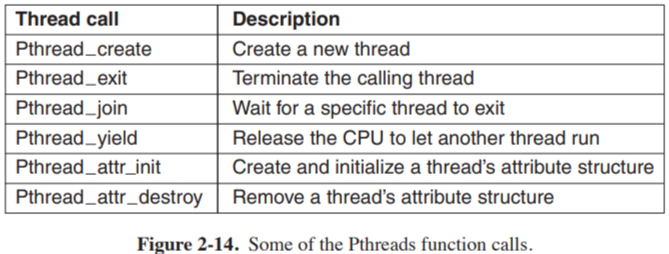
\includegraphics[width=1\linewidth]{pthreadFunctionCalls}}




\vfill \null
\columnbreak

\section{5. Inter-Process Communication (IPC)}

Given that processes frequently need to communicate, some need for communication, preferably in some well-structured way not using interrupts. Consider that cooperating processes have independent memory space, making IPC necessary.

\section{Common Communication Mechanisms}

\section{Shared Memory}
\begin{itemize}
\item \textbf{General Idea}: Process 1 creates shared memory region $M$, process 2 attaches $M$ to its own memory space. Both processes can now communicate using memory region $M$. Applicable to multiple processes.
\item $M$ behaves similar to normal memory region, any writes to region can be seen by all other parties.
\end{itemize}
\centerline{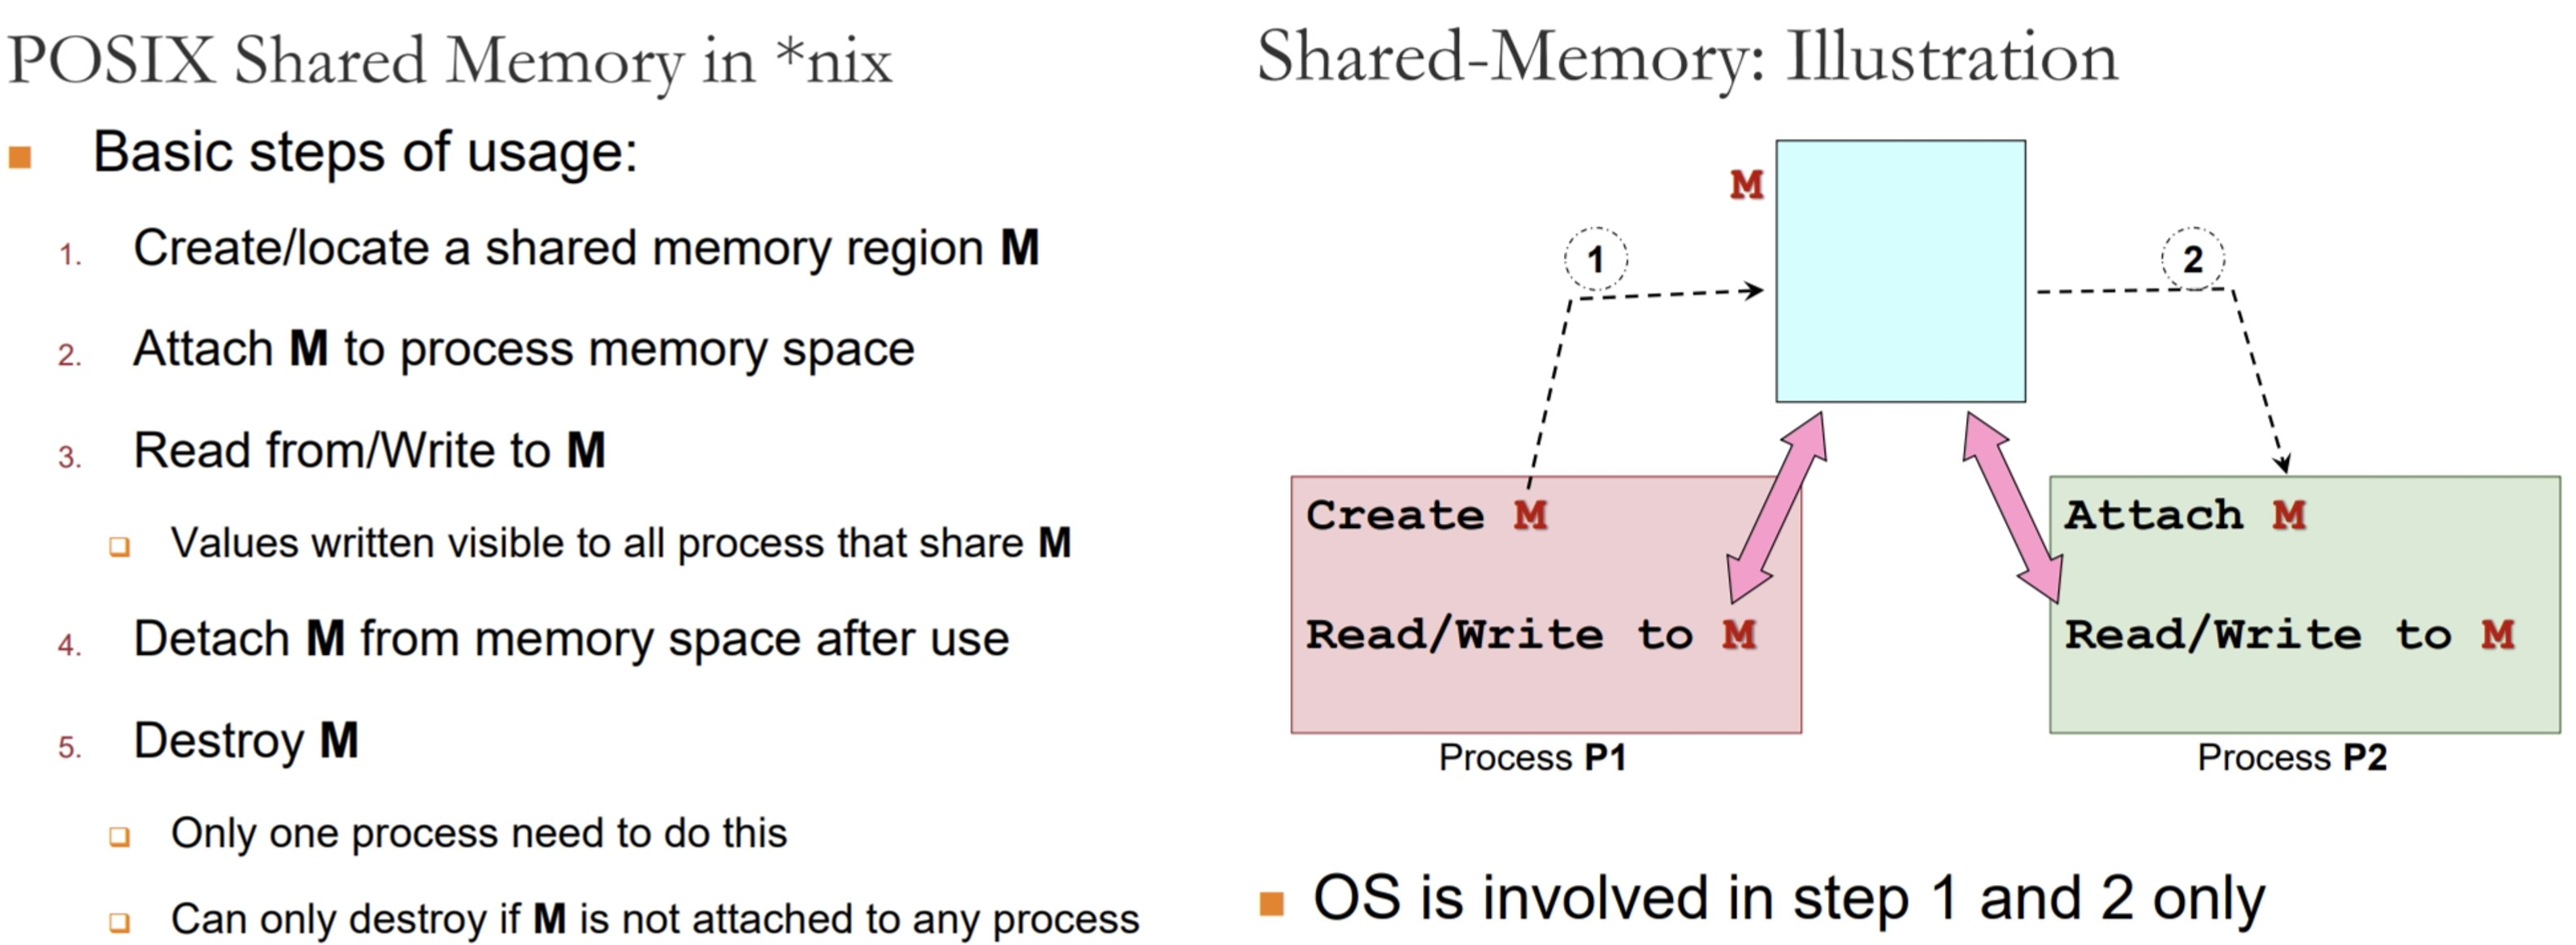
\includegraphics[width=1\linewidth]{sharedMemory}}
\begin{itemize}
\item \textbf{Advantages}:  \\
- Efficient, as only initial steps of create \& attach $M$ involves OS. \\
- Ease of use, as $M$ behaves as normal memory space, info of any size/type writable easily.
\item \textbf{Disadvantages}: \\
- Synchronization: Shared resource, need to sync access still. \\
- Implementation is harder.
\end{itemize}
\centerline{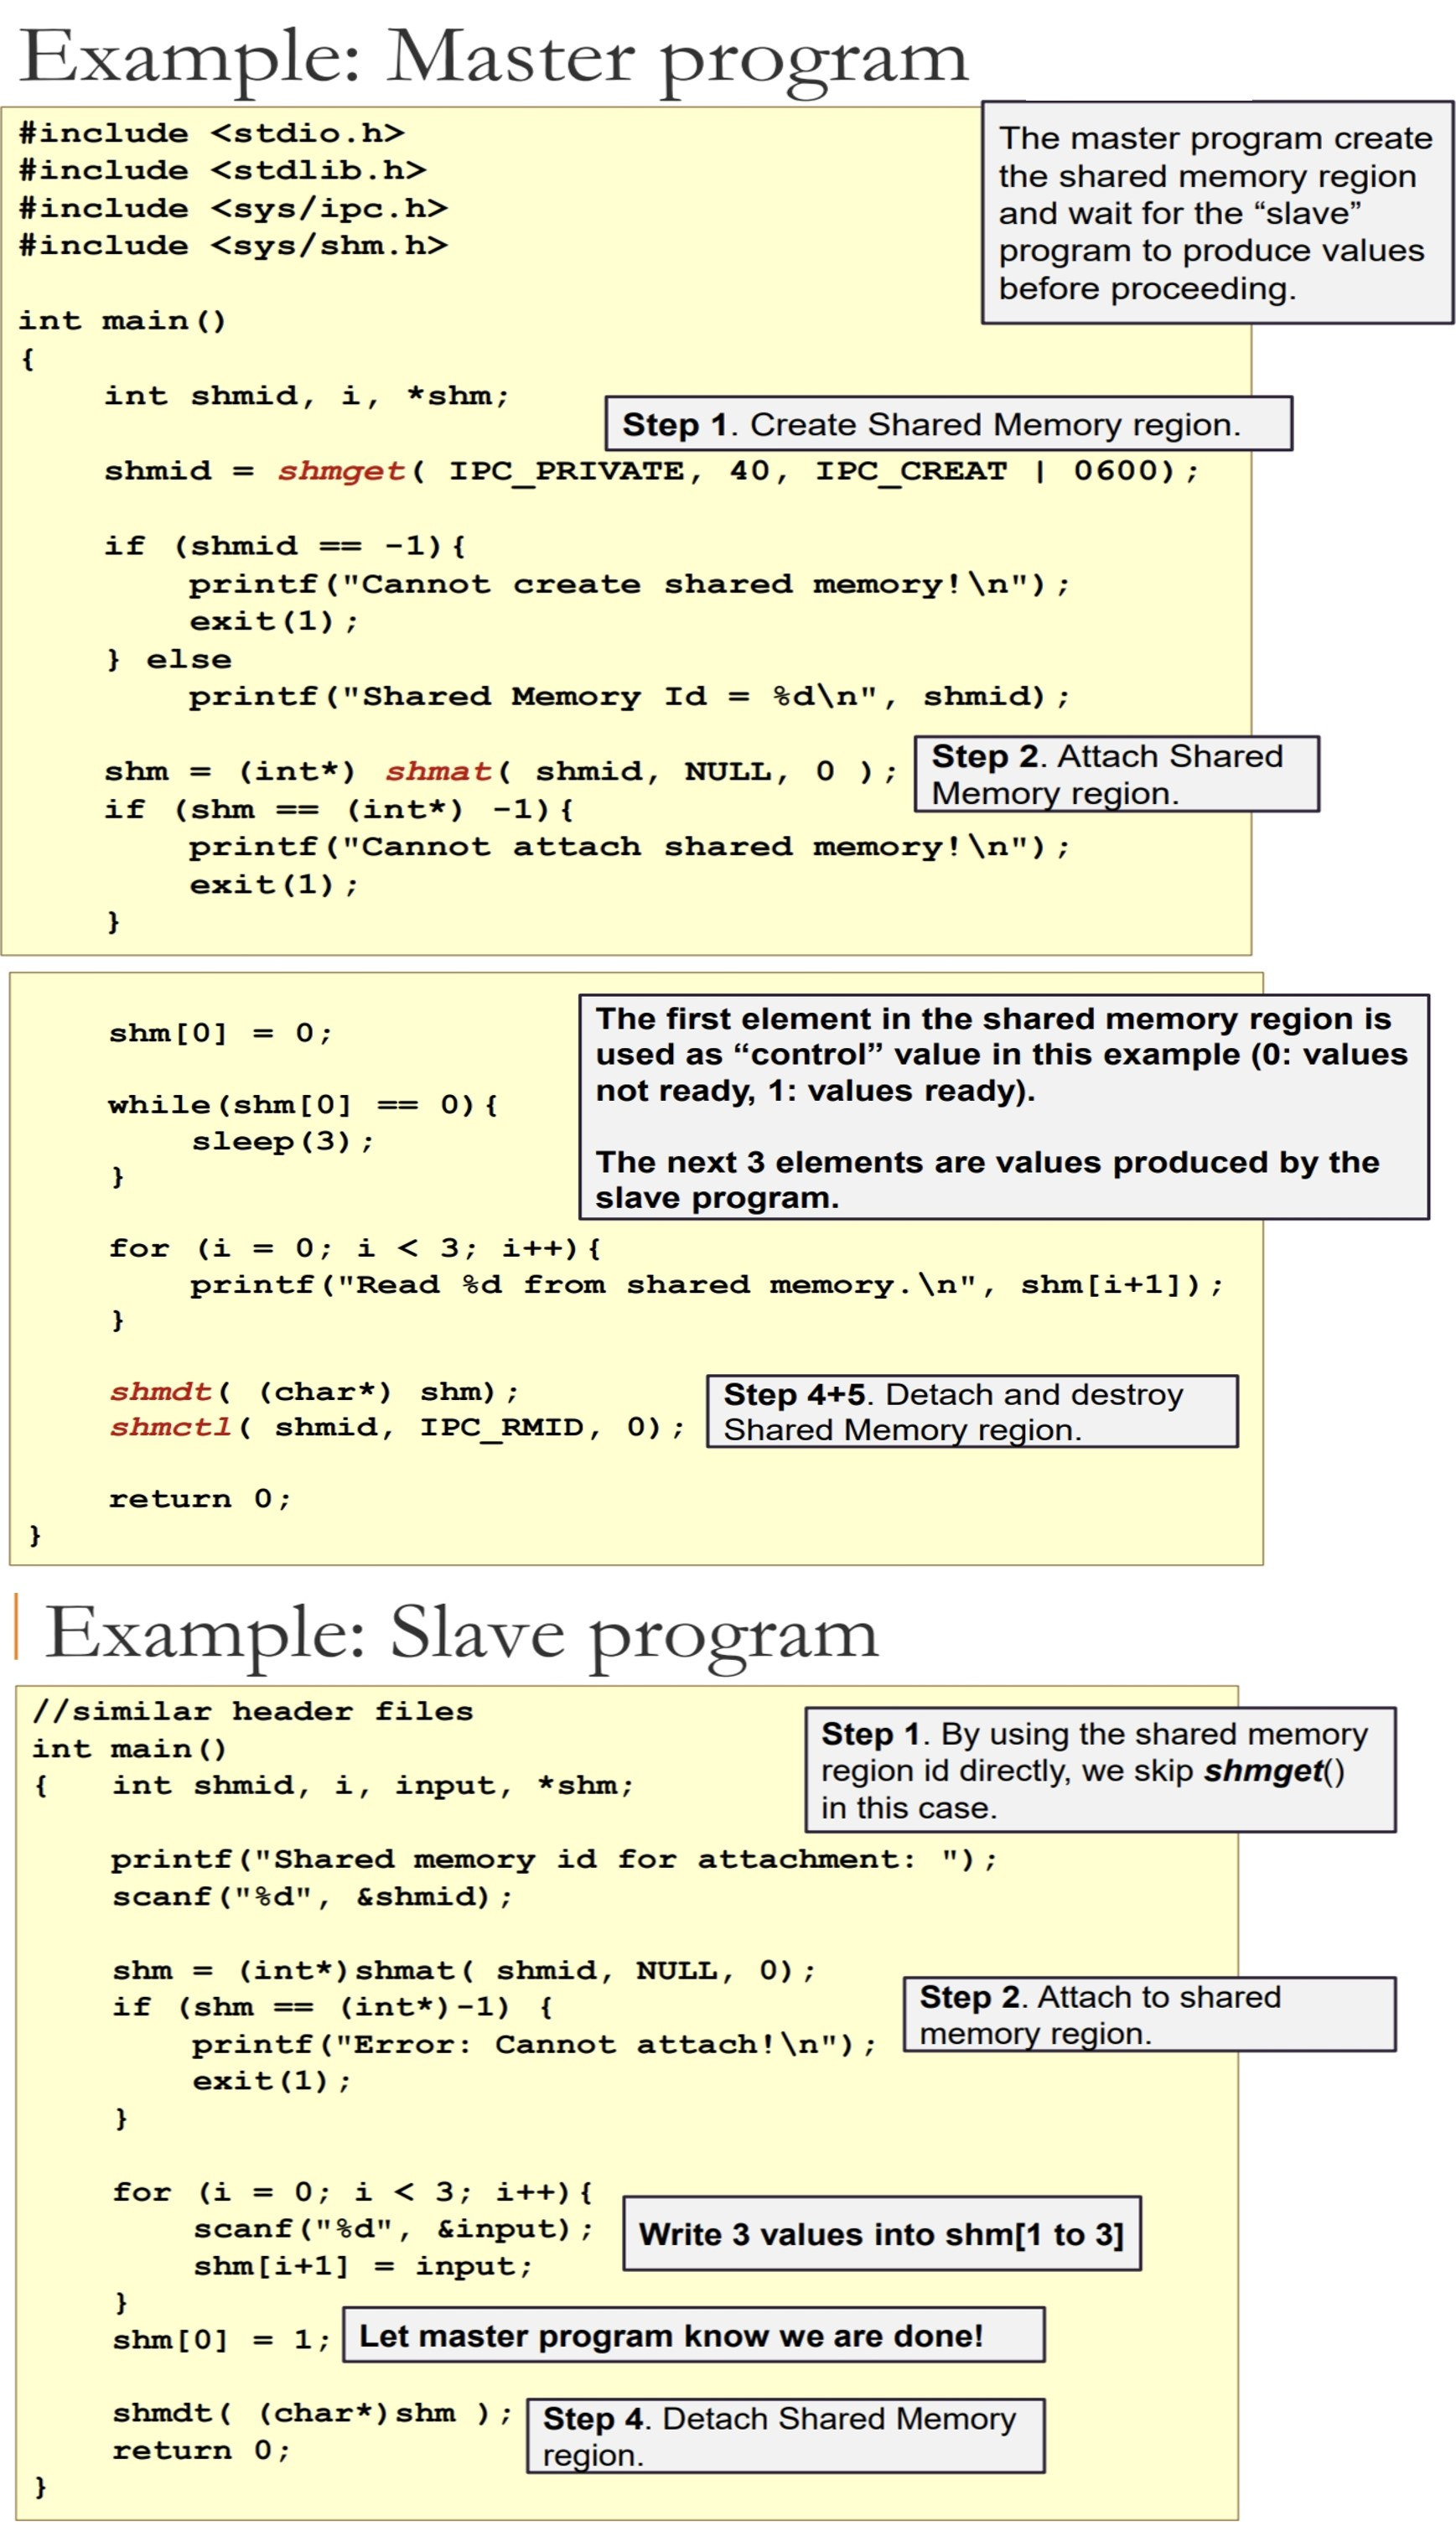
\includegraphics[width=0.60\linewidth]{sharedMemoryExample}}


\section{Message Passing}
\begin{itemize}
\item \textbf{General Idea}: Process 1 prepares, send message $M$. Process 2 receives it.
\item Message sending / receiving usually provided as system calls.
\item \textbf{Additional properties}: Naming (identify other party), synchronization (behavior of send/rec ops).
\item \textbf{Msg} has to be stored in kernel memory space. Each send/rec op needs to go through OS (system call).
\end{itemize}

\subsubsection{Direct Communication (Naming Scheme)}
\begin{itemize}
\item Sender/Receiver of message \textbf{explicitly names other party}.
\item E.g. \code{Send(P2, Msg)} \& \code{Receive(P1, Msg)}.
\item One link per pair of process, need know identity of other party.
\end{itemize}

\subsubsection{Indirect Communication (Naming Scheme)}
\begin{itemize}
\item Messages sent / recieved from message storage, \textbf{aka mailbox / port}.
\item E.g. \code{Send(MB, Msg)} \& \code{Receive(MB, Msg)}.
\item One mailbox can be shared among a number of processes
\end{itemize}

\subsection{Synchronization Behaviors}
\begin{itemize}
\item \textbf{Blocking Primitives (Synchronous)}: Sender blocked until message received, receiver blocked until message has arrived.
\item \textbf{Non-Block Primitives (Asynchronous)}: Sender resume operation immediately, receiver either receive, or indicate message not ready yet.
\end{itemize}

\begin{itemize}
\item \textbf{Advantages}: \\
- Portable, easily implemented on diff. processing env. \\
- Easier synchronization: Esp. when synchronous primitive used.
\item \textbf{Disadvantages}: \\
- Inefficient, require OS intervention \\
- Harder to use, less flexi, messages limited in size / format.
\end{itemize}

\section{Pipe (Unix Specific)}
\begin{itemize}
\item Unix process has 3 default communication channels: \\
- \textbf{stdin} (standard in): Commonly linked to keyboard input. \\
- \textbf{stderr} (standard error): Only used print out error msg. \\
- \textbf{stdout} (standard out): Commonly linked to screen. 
\end{itemize}
\centerline{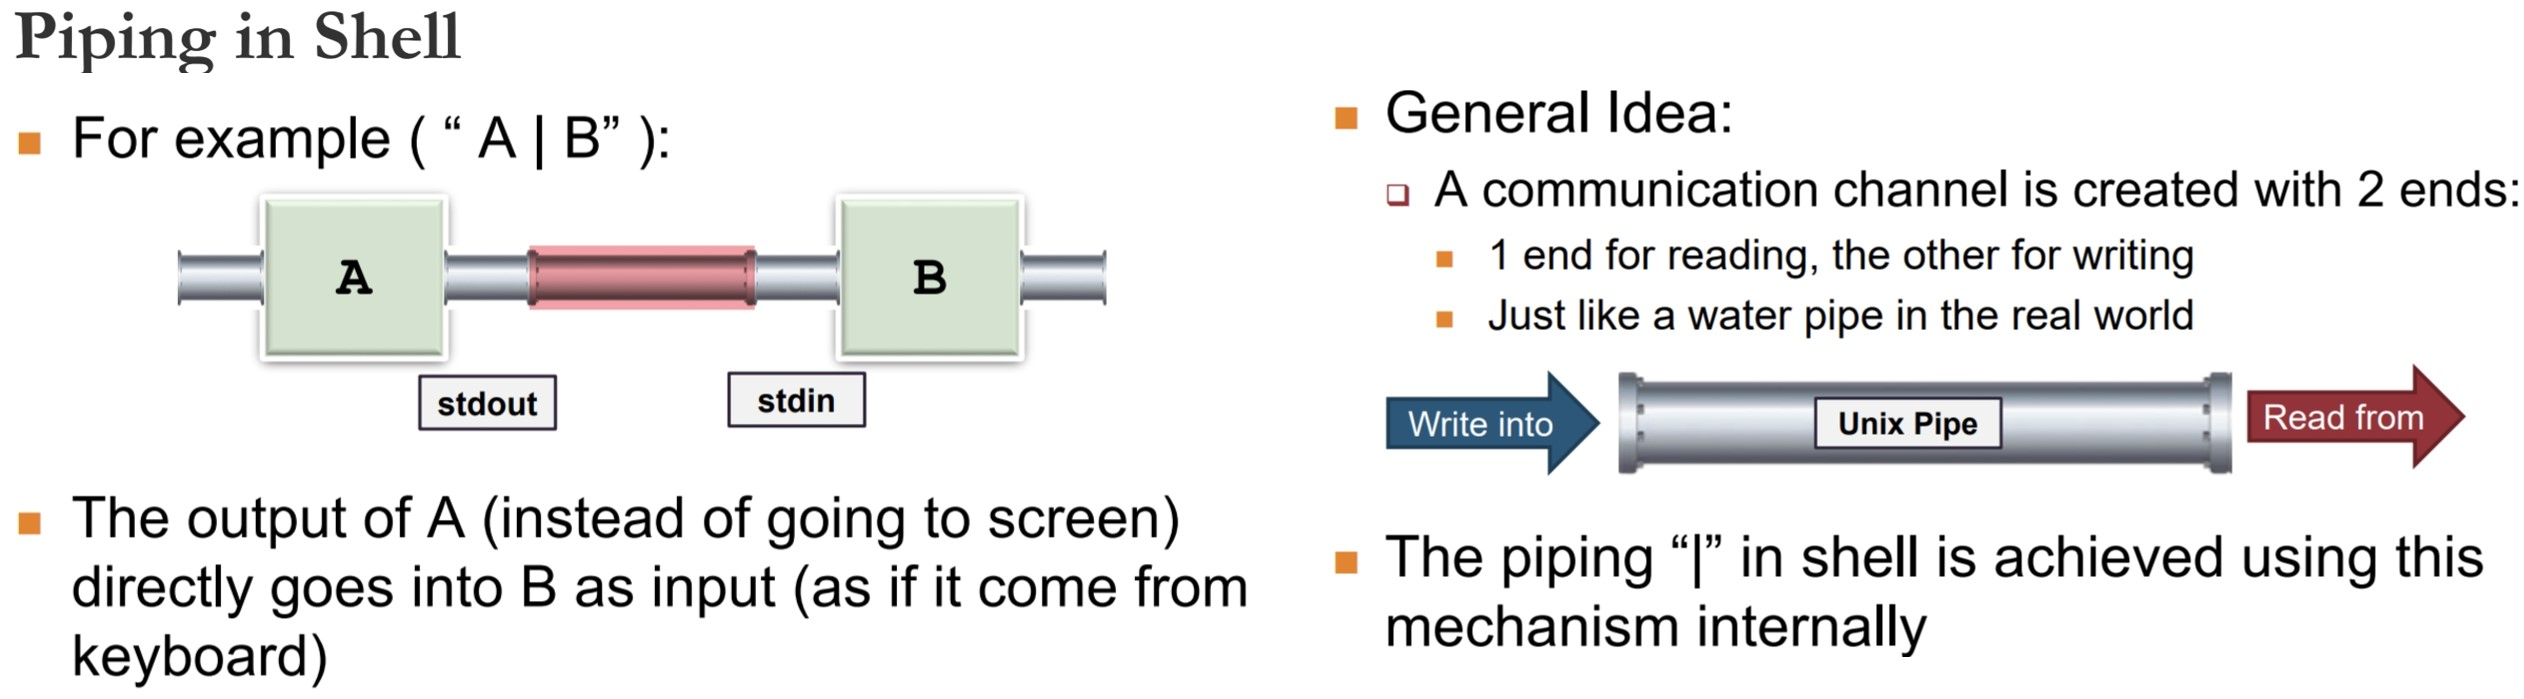
\includegraphics[width=0.90\linewidth]{piping1}}

\begin{itemize}
\item \textbf{Unix Shell Piping}: Unix shell provides $|$ symbol to link input/output channels of one process to another, aka \textit{piping}.
\end{itemize}

\centerline{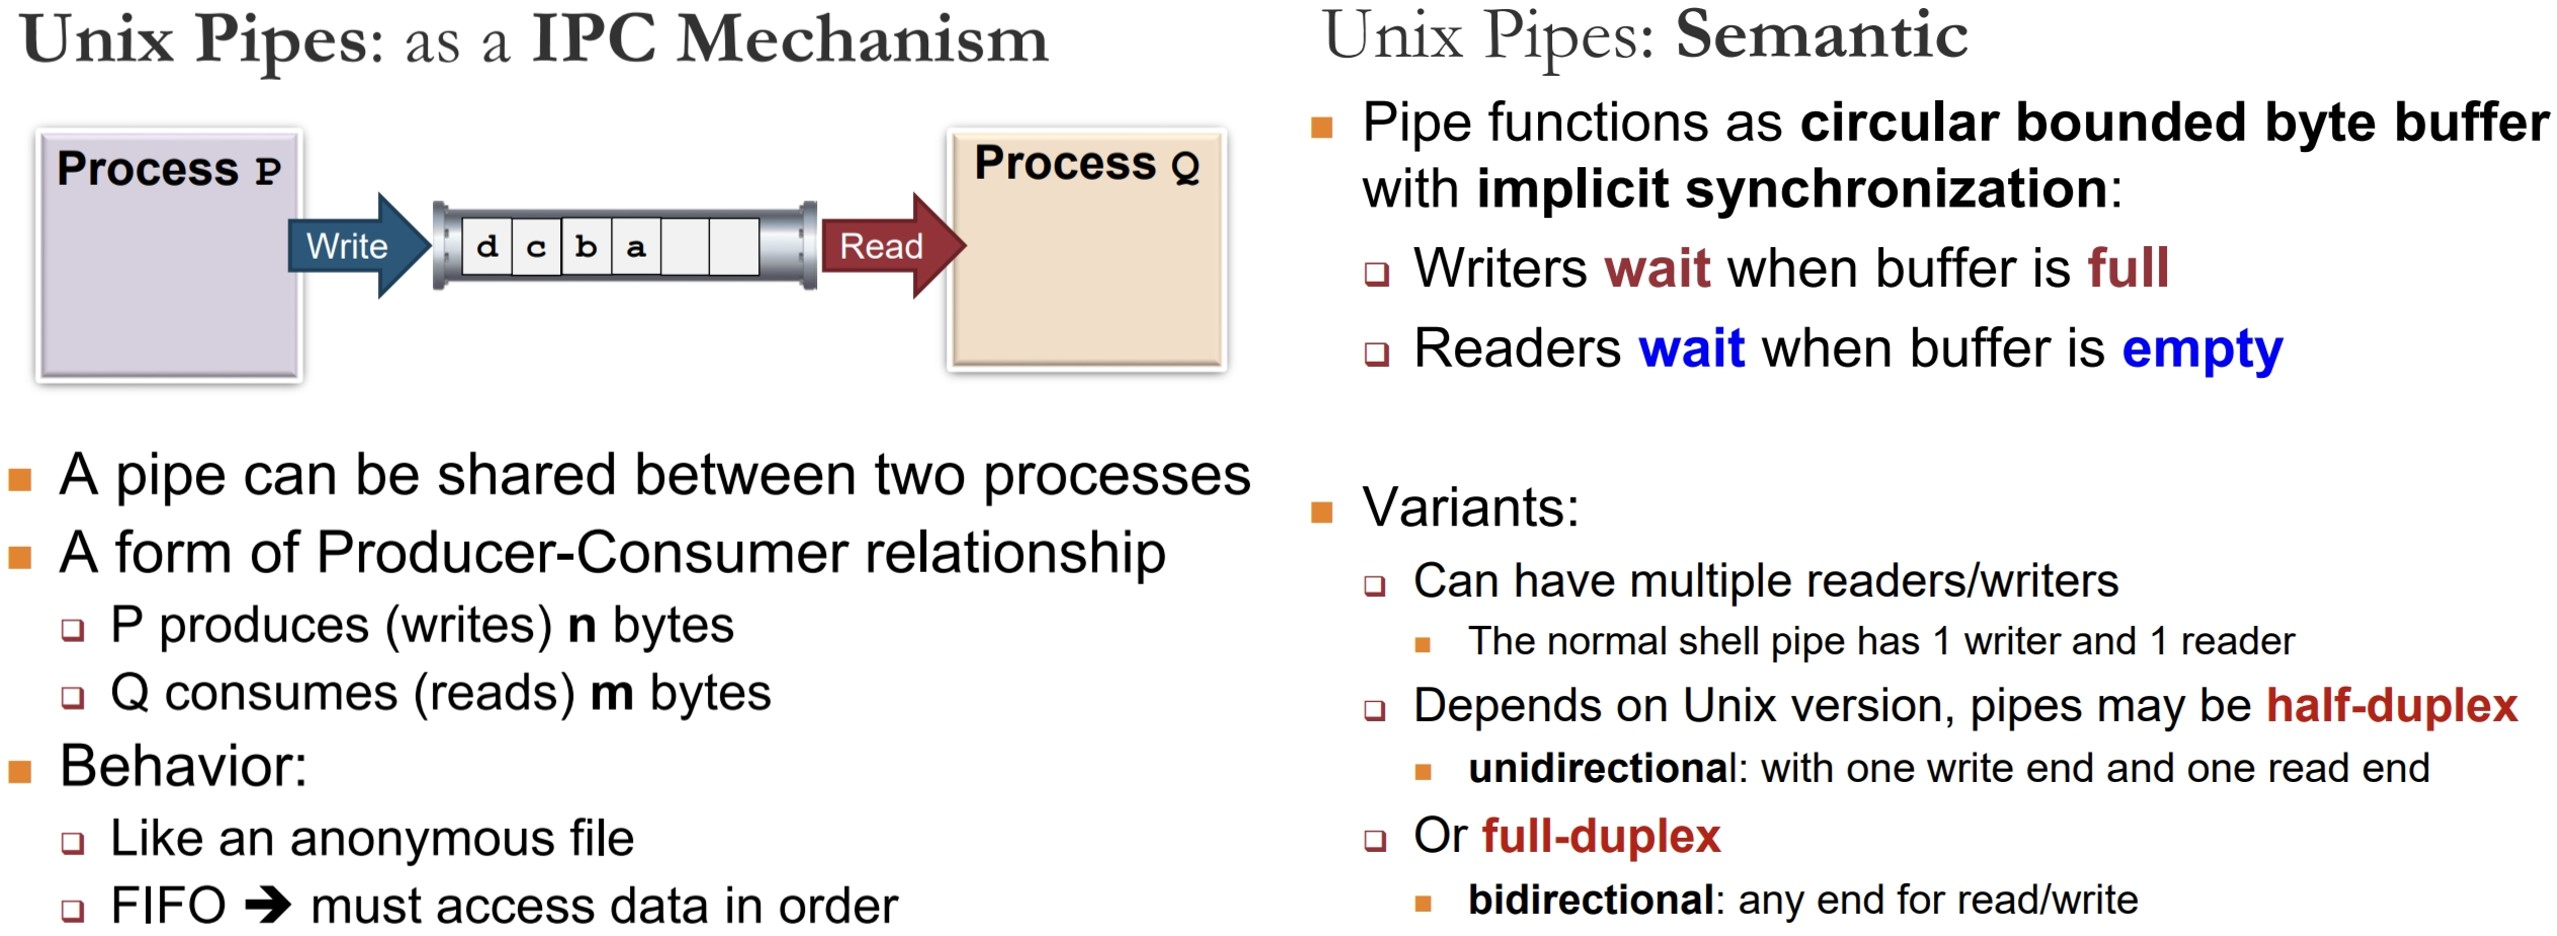
\includegraphics[width=1\linewidth]{piping2}}

\centerline{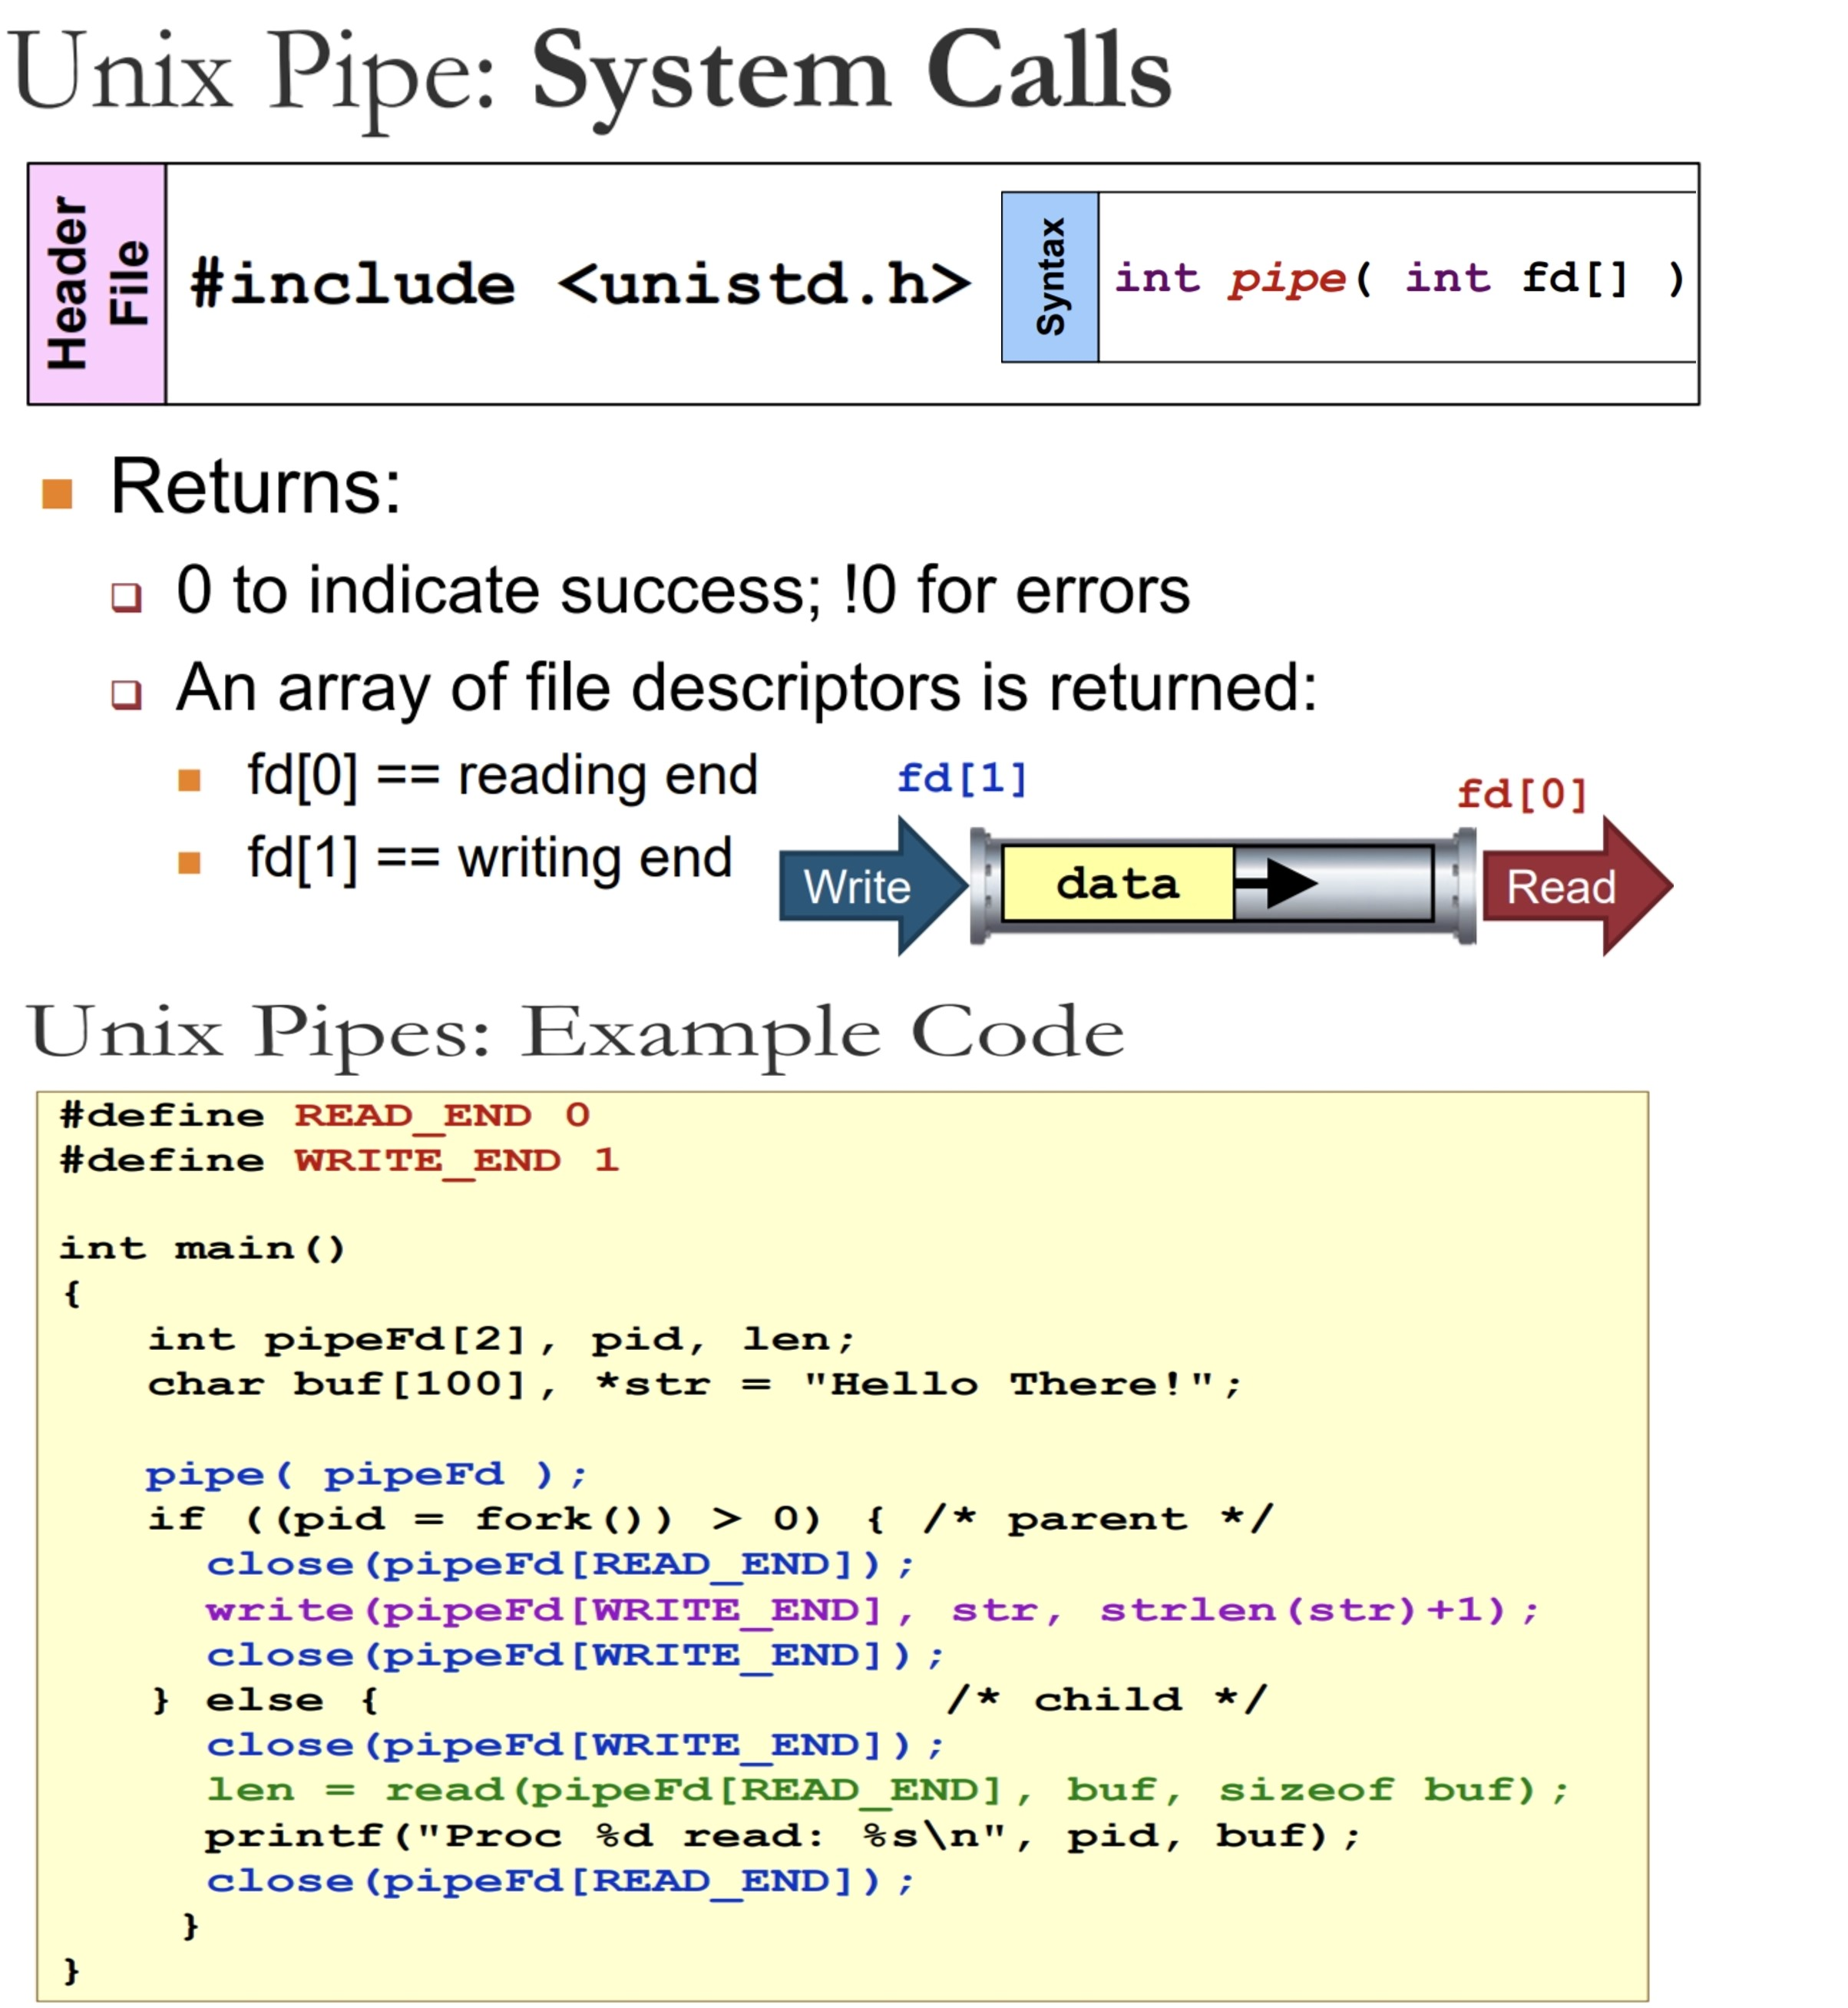
\includegraphics[width=0.8\linewidth]{piping3}}


\section{Signal (Unix Specific)}
\begin{itemize}
\item Form of IPC. \textbf{Asynchronous notification} regarding an event. Sent to process / thread.
\item Recipient of signal must handle signal by: Default set of handlers or user supplied handler.
\item \textbf{Common UNIX signals}: Kill, Stop, Continue, Arithm. error etc.
\end{itemize}
\centerline{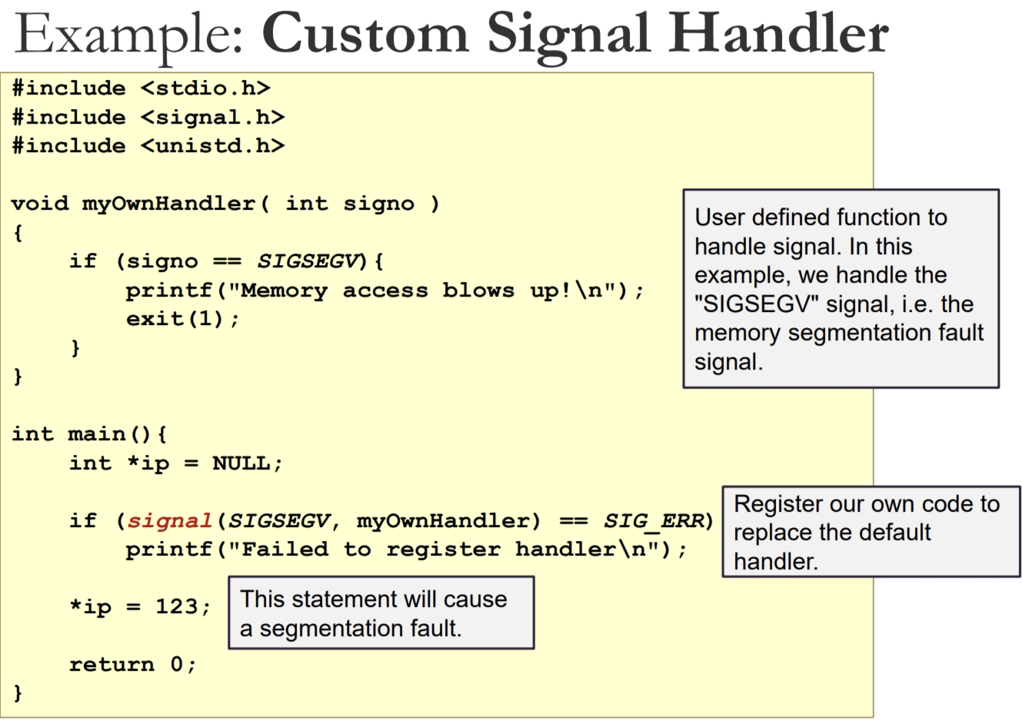
\includegraphics[width=0.8\linewidth]{customHandler}}


\vfill \null
\columnbreak


\section{6. Synchronization}

\textbf{Problems with Concurrent Execution}: When process execute in interleaving fashion AND share a modifiable resource, can cause \textbf{synchronization problems}. 
\begin{itemize}
\item Single sequential process execution deterministic, concurrent processes execution may be non-deterministic.
\item \textbf{Race Condition}: When final result depends on who runs precisely when. 
\end{itemize}

\subsection{Critical Regions / Sections}
\begin{itemize}
\item \textbf{Critical Section}: Part of the program where shared memory is accessed (with race condition).
\item Incorrect execution is due to \textbf{unsynchronized access to shared modifiable resource}.
\item If no two processes in their CS at same time, we can avoid races.
\item \textbf{4 Conditions of good Critical Section / Region (CS) Implementation:}
	\begin{enumerate}
	\item \textbf{Mutual Exclusion}: No two processes simultaneously inside their CS.
	\item \textbf{Progress}: If no process in CS, one waiting process granted access.
	\item \textbf{Bounded Wait}: No process waits forever to enter its CS.
	\item \textbf{Independence}: No process outside CS may block any process.
	\end{enumerate}
\item \textbf{Symptoms of Incorrect Synchronization:}
	\begin{itemize}
	\item \textbf{Deadlock}: All processes blocked, no progress.
	\item \textbf{Livelock}: Process keep changing state to avoid deadlock, make no progress (dl avoidance mechanism), typically process not blocked.
	\item \textbf{Starvation}: Some processes blocked forever.
	\end{itemize}
\end{itemize}

\subsection{Critical Section Implementations}
\begin{itemize}
\item \textbf{Assembly Level Implementations:} Mechanism provided by processor.
\item \textbf{High Level Language Implementations:} Utilizes only normal programming constructs. (E.g. CS lock using normal variables)
\item \textbf{High Level Abstraction:} Abstracted mechanisms that provide additional useful features (E.g. abstract data types, provided as library calls, and involve system calls). 
\end{itemize}

\section{6.1 Assembly Level Implementation}

\subsection{Test and Set (TSL) Instruction}
Common machine instruction to aid synchronization: TSL RX,LOCK. (Test and Set Lock). \code{TestAndSet Register, MemoryLocation}
\begin{itemize}
\item \textbf{Behavior}: Load current content at \textbf{MemoryLocation} into \textbf{Register}, and stores a 1 into \textbf{MemoryLocation}
\item \textbf{Atomic}: Performed as a single machine operation, indivisible.
\item Assume equivalent high level lanugage ver of \textbf{TSL}:
\end{itemize}
\centerline{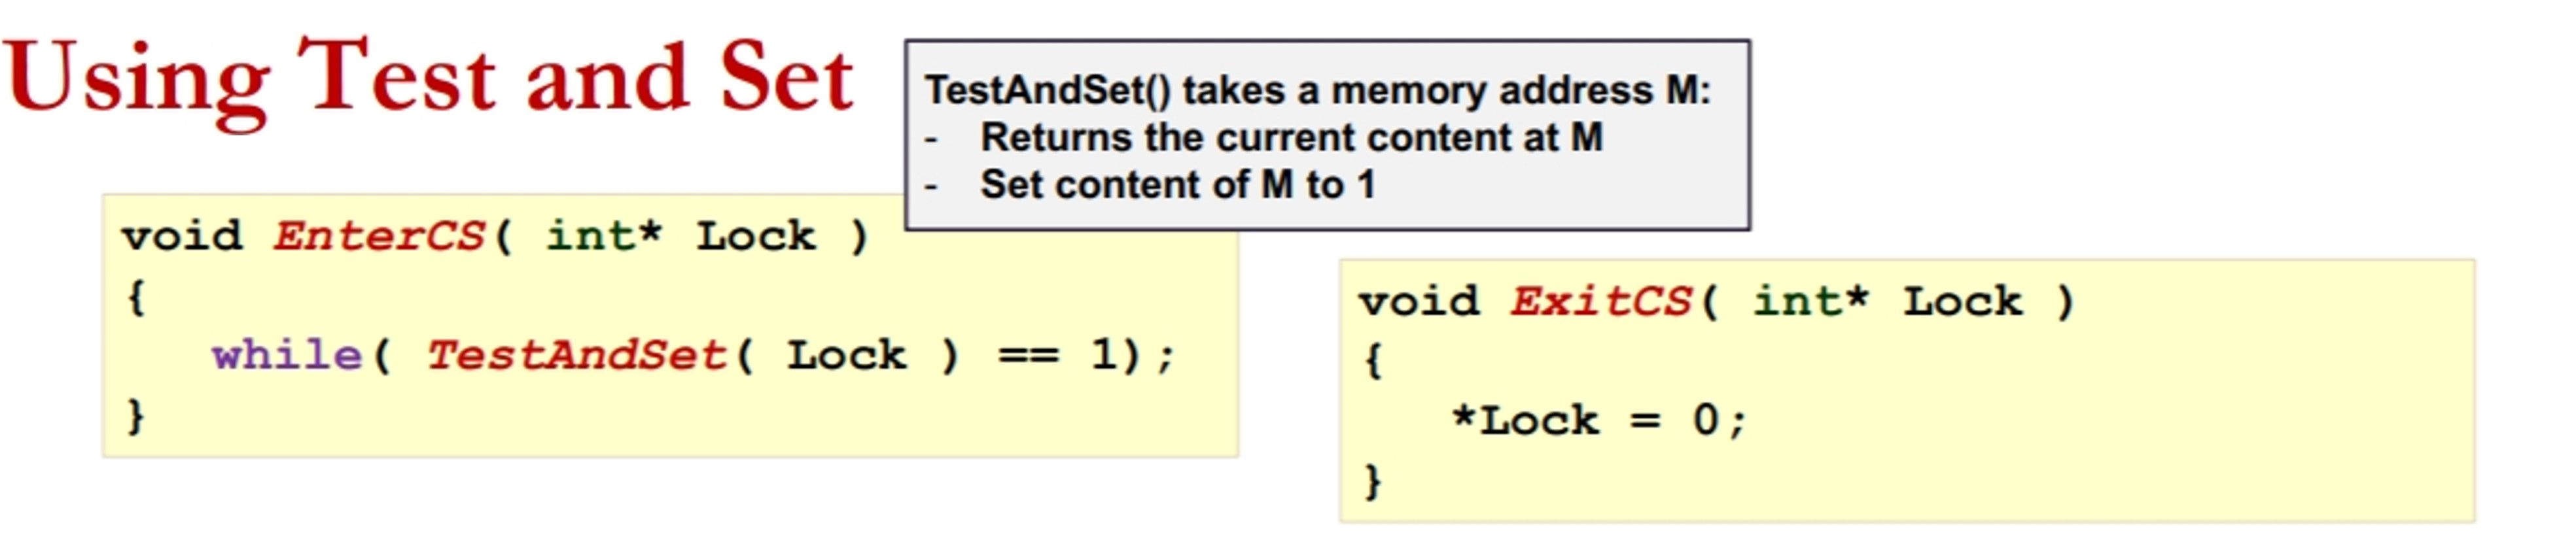
\includegraphics[width=1\linewidth]{testSet}}
\begin{itemize}
\item \textbf{How Implementation works}: Before entering CS, a process calls enterCS, busy wait until lock is free; then it acquires the lock and returns. After leaving CS process calls ExitCS, which stores a 0 in lock. 
\item \textbf{Inefficient}: Employs busy waiting, wasteful use of processing power.
\item \textbf{Variants of instruction}: \code{CompareandExchange}, \code{AtomicSwap}, \code{Load Link}.
\end{itemize}

\section{6.2 High Level Language Implementation}

\subsection{Bad: Lock Variables}
Have a single, shared (lock) variable, initially 0. When entering CS, test lock and sets to 1.Thus, 0 means no process in CS, 1 means some process in CS.
\smallskip
\centerline{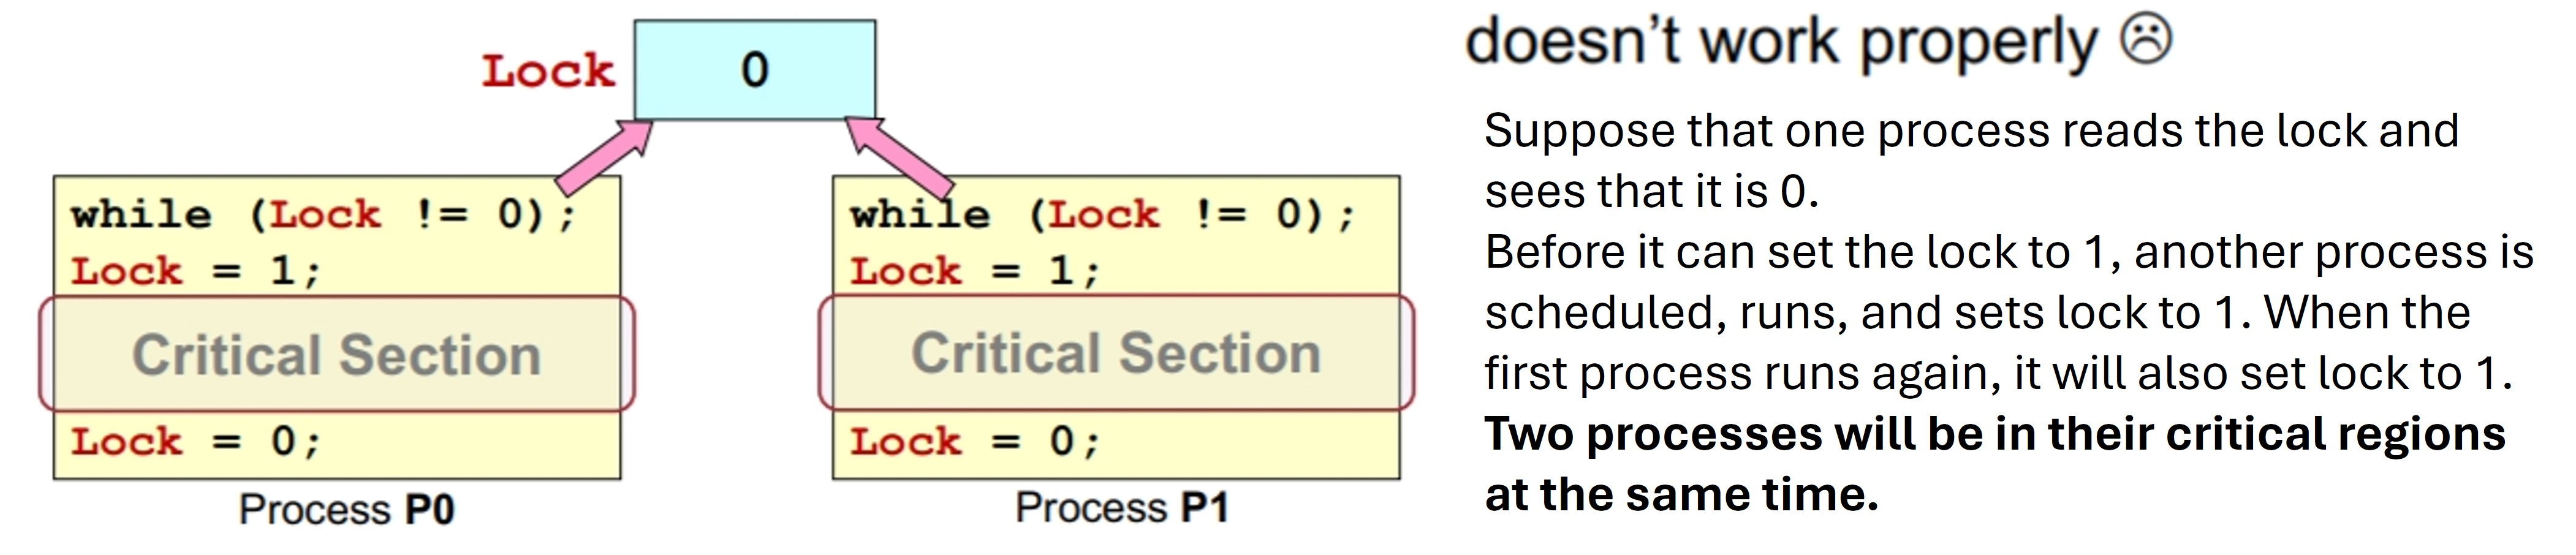
\includegraphics[width=1\linewidth]{HLL1}}

\subsection{Bad: Lock Variables with Interrupts Disabled}
Solve the problem by preventing context switch, by disabling interrupts.
\smallskip
\centerline{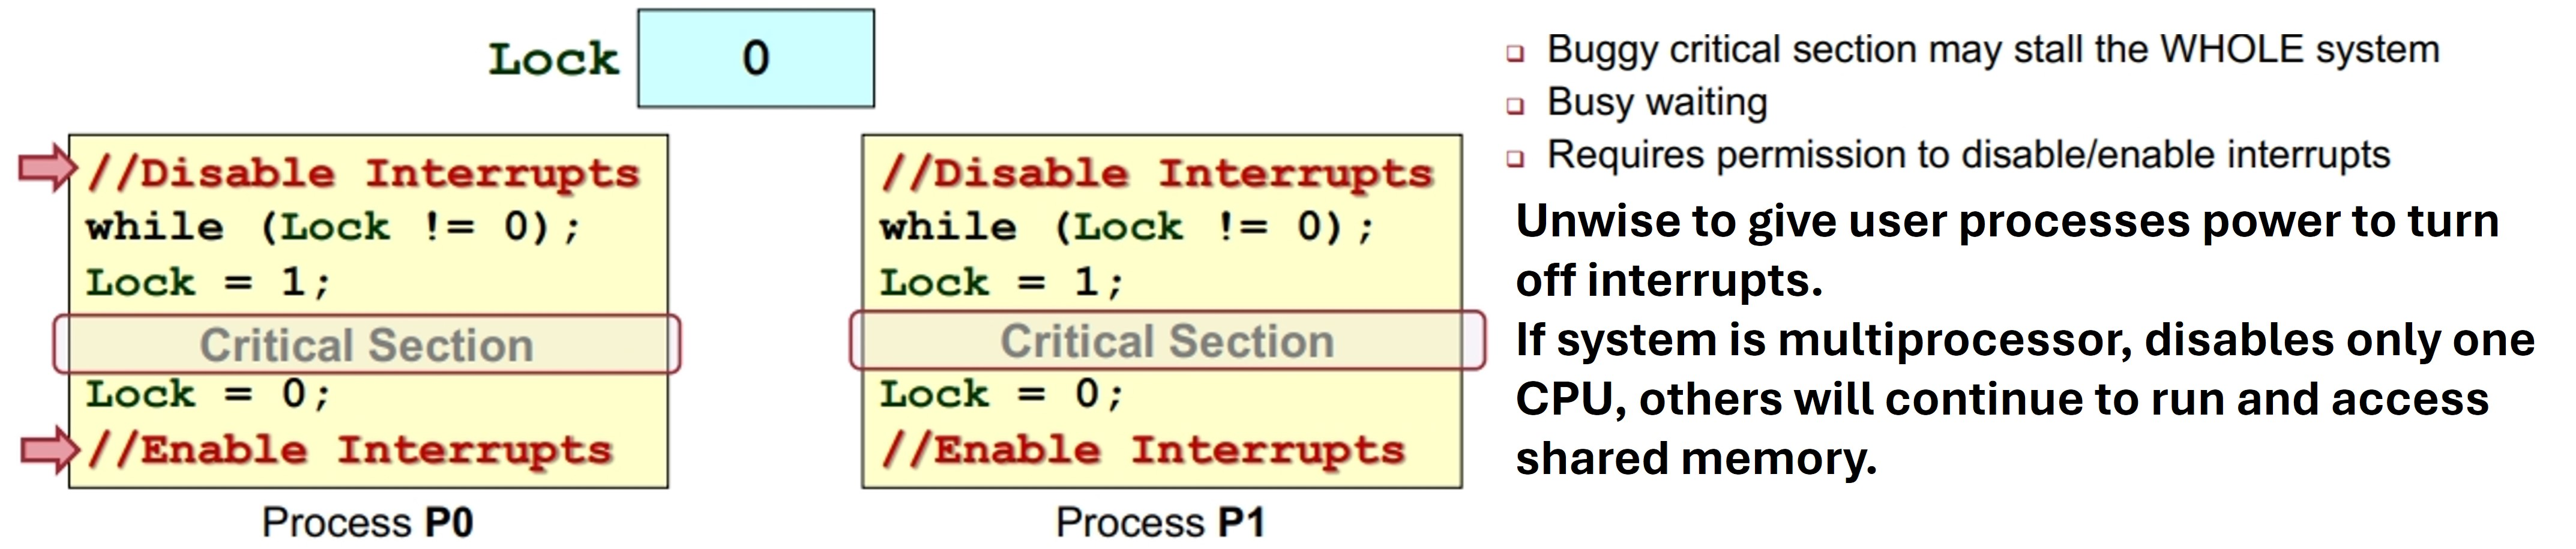
\includegraphics[width=1\linewidth]{HLL2}}

\subsection{Bad: Strict Alternation}
The integer variable turn, initially 0, keeps track of whose turn it is to enter the critical region and examine or update the shared memory.
\smallskip
\centerline{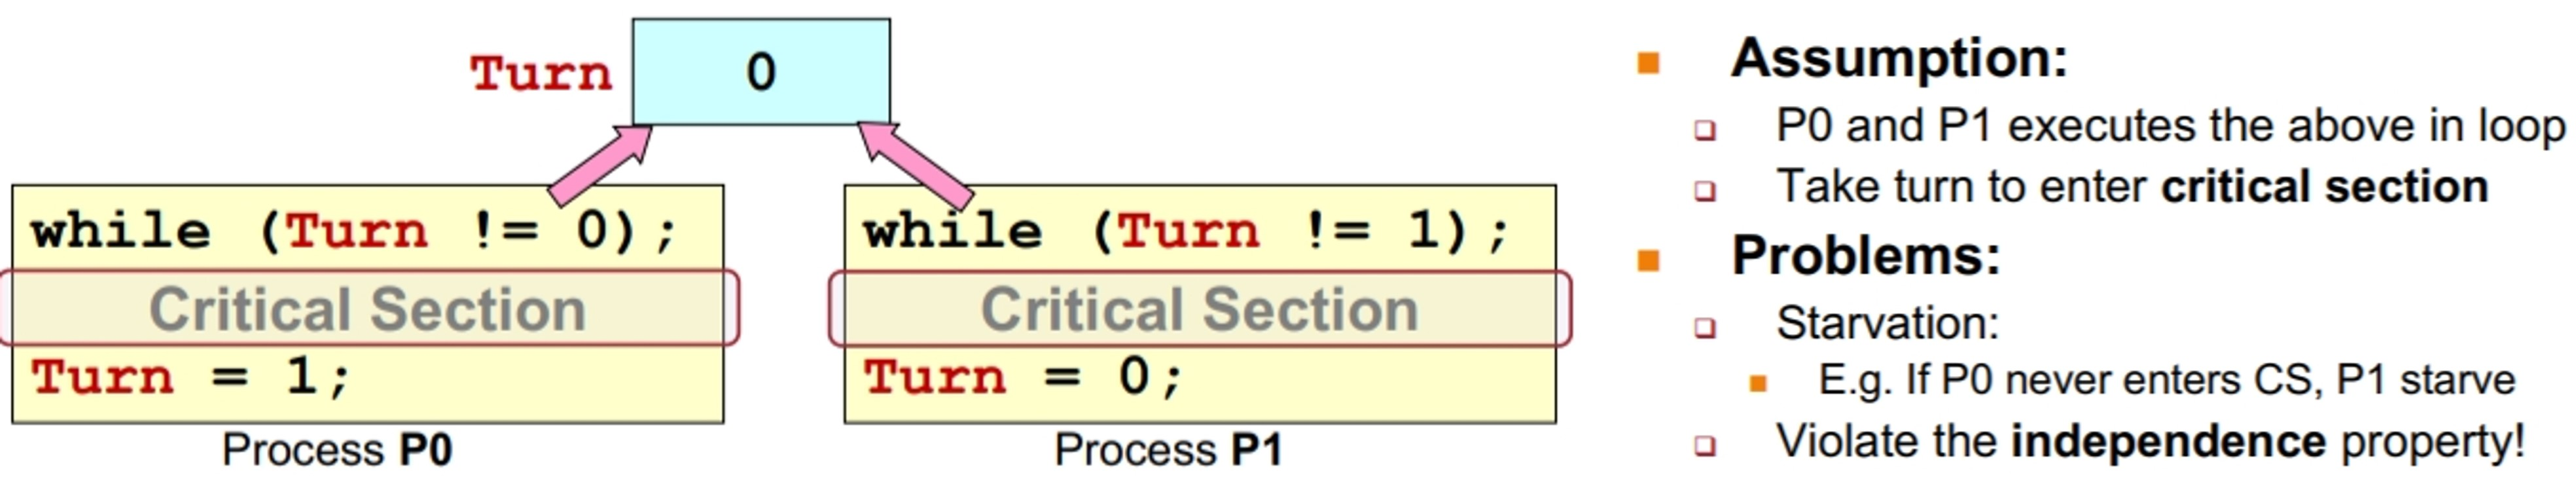
\includegraphics[width=1\linewidth]{HLL3}}
\textbf{Independence property violated}: After P0 enters CS, sets turn to 1, and wants to enter CS again, needs to wait for P1 to enter its CS to set turn to 0. If P1 does not enter CS, turn stuck at 1, P0 starves.

\subsection{Bad: Sub-Peterson Algorithm (without turn)}
Leading up to peterson's algorithm. Use global shared array Want, if process wishes to enter CS, set Want[n] to 1.
\smallskip
\centerline{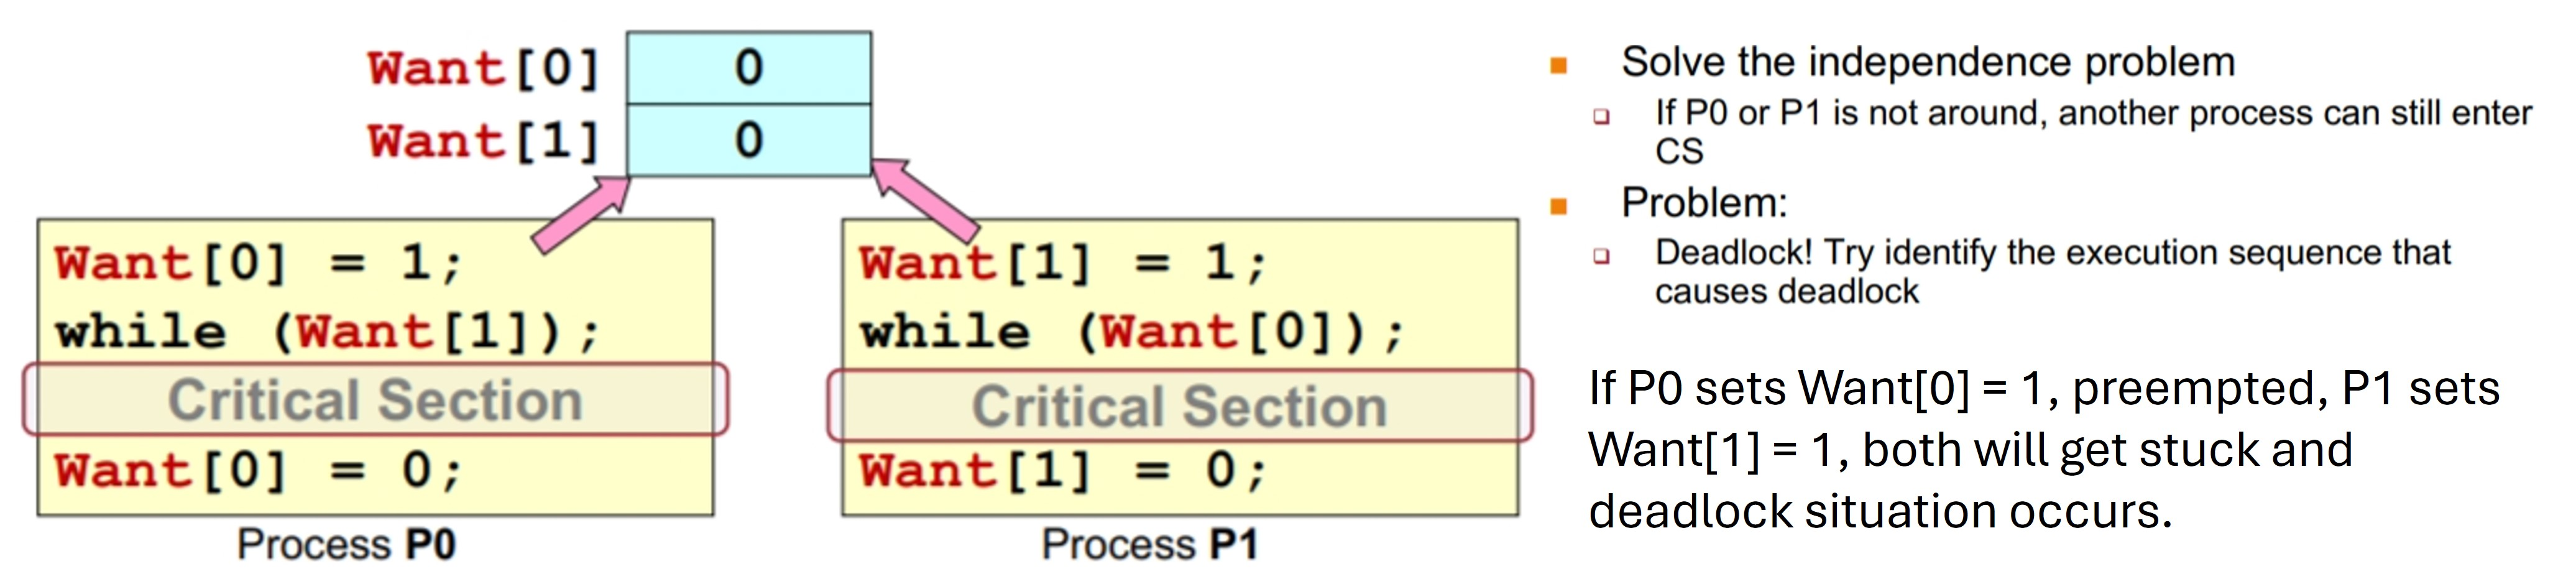
\includegraphics[width=1\linewidth]{HLL4}}

\subsection{Good: Peterson's Algorithm}
Assume that writing to Turn is an \textbf{atomic operation}.
\smallskip
\centerline{\includegraphics[width=1\linewidth]{Peterson}}
Process can store their process number, or the other process number in turn. 
Consider both processes trying to enter CS almost simultaneously. 
Both store in turn variable. Whichever store done last is the one that counts; first one overwritten and lost. After, only one can enter CS, the other will loop. 

\columnbreak

\section{6.3 High Level Abstraction Implementation}

\subsection{Semaphore}

\subsubsection{Understanding}
\begin{itemize}
\item E.W. Dijkstra proposed using semaphore to count the number of wakeups saved for future use. (Processes sleep while waiting for shared resource).
\item \textbf{Atomic}: Once a semaphore operation started, no other process can access semaphore until operation has completed or blocked.
\end{itemize}
\centerline{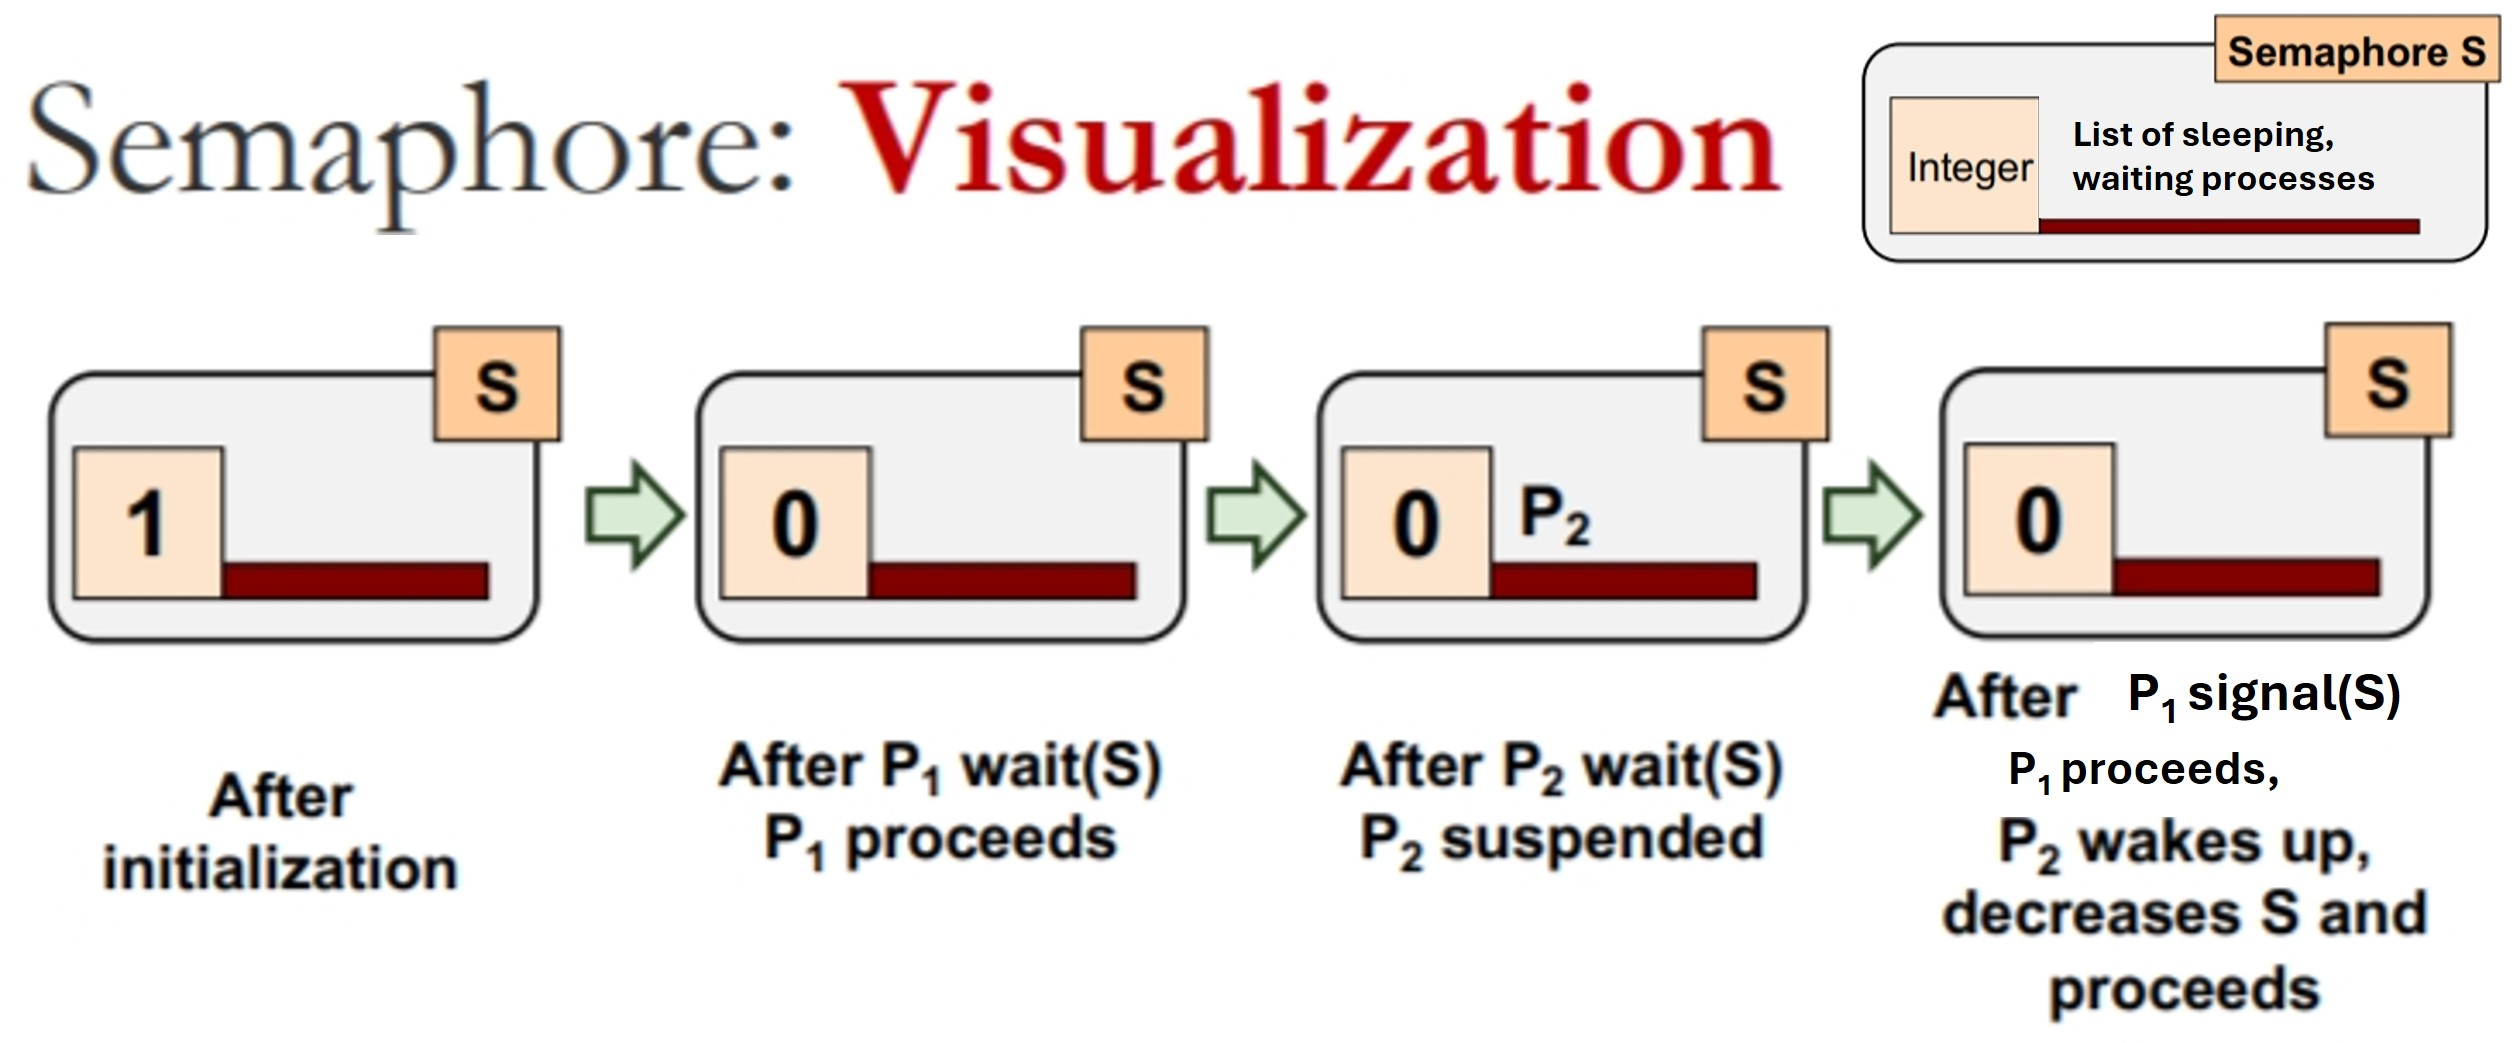
\includegraphics[width=0.7\linewidth]{semaphore}}

\textbf{Semaphore}: A generalized synchronization mechanism that specify behavior and not implementation. Provides a way to block a number of processes, which will then be known as \textbf{sleeping processes}.

\begin{itemize}
\item Semaphore S seen as a "protected integer", with non-negative initial value. 
\item A general semaphore (aka counting semaphore) can have values $S \geq 0$. A binary semaphore or mutex has values $S = 0$ or 1.
\end{itemize}

\subsubsection{Wait(S)}
Takes in a semaphore. If semaphore value is $\leq$ 0, blocks current process. \\
Decrements the value when it proceeds. Atomic operation. Aka \textbf{down()}.

\subsubsection{Signal(S)}
Takes in a semaphore, wakes up one sleeping process (if any) and increments the semaphore value. This is an atomic operation and never blocks. Aka \textbf{up()}.

\subsection{Semaphore Invariant}
\begin{itemize}
\item $S_{current} \geq 0$
\item $S_{current} = S_{initial} + \#signal(S) - \#wait(S)$
\item $\#signal(S)$ is number of $signal()$ executed, $\#wait(S)$ is number of $wait()$ operations completed.
\end{itemize}

\subsection{Mutex (Binary Semaphore Usage)}
\begin{itemize}
\item Set binary semaphore $s = 1$, for any process, do \textbf{wait(s)} before entering CS, and \textbf{signal(s)} after finishing CS.
\item S can only be 0 or 1, deduced by semaphore invariant.
\item This usage known as \textbf{mutex} (Mutual Exclusion)
\end{itemize}
\centerline{\includegraphics[width=0.95\linewidth]{mutexProof}}
\begin{itemize}
\item \textbf{Possible Deadlock}: Note incorrect usage of semaphore may still result in deadlock, e.g. incorrect interleave usage of semaphore.
\item \textbf{Conditional Variable}: Similar to semaphore, but allows process to wait for some event to happen. Once event happens, broadcast made to wake up all waiting tasks.
\end{itemize}

\section{6.4 Classical Synchronization Problems}

\subsection{Producer-Consumer Problem}
Processes share a bounded buffer of size K. Producers produce items to insert in buffer, only when the buffer
is not full. Consumers remove items from buffer, only when the buffer is not empty. \textit{How to sync the two?}

\subsubsection{Busy Waiting Solution (Inefficient)}
\centerline{\includegraphics[width=0.95\linewidth]{PCBusyWaiting}}

\subsubsection{Blocking Solution}
Solution uses three semaphores, one called (\textit{notFull}) for counting empty slots, one called (\textit{notEmpty}) for counting full slots, and one called \textit{mutex} to make sure producer and consumer do not access the buffer at the same time. 
\begin{itemize}
\item \textit{NotFull} is initially equal to the number of slots in the buffer, \textit{NotEmpty} is initially 0, and \textit{mutex} is initially 1.
\item When producing item, wait(notFull), which decrements. Then, acquire mutex. After producing, signal (release) mutex, and signal(notEmpty), causing it to increment.
\end{itemize}
\centerline{\includegraphics[width=0.95\linewidth]{PCBlocking}}

\subsection{Readers and Writers Problem}
Processes share a data structure $D$, where readers can access and read information from D together, while
writers must have exclusive access to $D$ to write information. \textit{How to sync the two?} \\ \smallskip
\centerline{\includegraphics[width=1\linewidth]{ReaderWriter}}
\begin{itemize}
\item \textbf{Problem}: As long as at least one reader active, subsequent readers admitted. Writer kept suspended until no reader is present. Writer may never get in.
\item \textbf{Rectification}: Program could be written slightly differently: when reader arrives and a writer is waiting, the reader suspended behind writer
instead of being admitted immediately. Writer waits for readers active to finish, but not readers after. Disadvantage is less concurrency and thus lower performance. 
\end{itemize}

\subsection{Dining Philosophers}
Five philosophers are seated around a table, and there are five single chopsticks placed between each pair
of philosophers. When any philosopher wants to eat, he/she will have to acquire both chopsticks from his/her left and right. \\
\textit{How can we have a deadlock-free and starvation-free way to allow the philosophers to eat freely?}

\subsubsection{Obvious Wrong Solutions}
\begin{itemize}
\item \textbf{Wait till fork is available}: Obvious solution is wrong. If all five philosophers take their left forks simultaneously. None will be able to take their right forks, and there will be a deadlock.
\item \textbf{After taking left fork, check right fork. If not available, put down left one, wait, and repeats}: Also fails, for different reason, if all philosophers start algorithm simultaneously, will cause livelock, fail to make progress, cause starvation. 
\item \textbf{Use single mutex}: Before acquiring forks, wait(mutex), after putting down, signal(mutex). While no deadlock, no starvation, It has perfomance bug, only one can eat at an instant. With five forks, at least two philosophers can eat at same time.
\end{itemize}

\subsubsection{Tanenbaum Solution}
The solution presented is deadlock-free and allows the maximum parallelism for an arbitrary number of philosophers.
\begin{itemize}
\item It uses an array, state, to keep track of whether a philosopher is eating, thinking, or hungry (trying to acquire cultery forks).
\item A philosopher may move into eating state only if neither neighbor is eating. Philosopher i’s neighbors are defined by the macros LEFT and RIGHT. In
other words, if i is 2, LEFT is 1 and RIGHT is 3.
\item The program uses an array of semaphores, one per philosopher, so hungry philosophers can block if the needed forks are busy.
\end{itemize}
\medskip
\centerline{\includegraphics[width=1\linewidth]{DiningP}}

\subsubsection{Limited Eater Solution}
\centerline{\includegraphics[width=1\linewidth]{DiningP2}}

\columnbreak

\section{6.5 Synchronization Implementations}
POSIX Implementations in Unix: \\ \medskip
\centerline{\includegraphics[width=1\linewidth]{POSIXsemaphore}}
\smallskip
\begin{itemize}
\item Programming languages with thread support will 
have some forms of synchronization mechanism
\item \textbf{Examples:}
	\begin{itemize}
	\item Java: all object has built-in lock (mutex) (monitor), synchronized method access, etc
	\item Python: supports mutex, semaphore, conditional variable, etc
	\item C$++$: Added built-in thread in C$++$11; Support mutex, conditional variable
	\end{itemize}
\end{itemize}

\vfill \null
\columnbreak

\section{7. Memory Management}
How OSes create abstractions from memory and how they manage them.

\section{7.1 Memory}
\begin{itemize}
\item \textbf{Physical memory storage}: Random Access Memory (RAM) accessible in O(1), think as an array of bytes, with \textbf{physical address} as "unique index".
\item \textbf{Contiguous memory region}: Interval of consecutive addresses.
\item \textbf{Memory hierarchy}: OS abstracts hierarchy into useful mode, and manages it.
\end{itemize}
\textbf{Binding of Memory Address for executable:} Executable contains code (text), data layout (data), that has been compiled by the compiler into machine code. This is \textit{load and run} into the main memory when we execute. 
\\ \textbf{Two types of data in a process}:
\begin{enumerate}
\item \textbf{Transient} Data: Valid for limited duration (e.g. function params, var)
\item \textbf{Persistent} Data: Valid for duration of program unless removed (e.g. global var, dynamically allocated memory).
\end{enumerate}

\textbf{OS needs to perform the following tasks}:
\begin{itemize}
\item Allocate memory space to new processes
\item Manage memory space for processes
\item Protect memory space of processes from each other
\item Provides memory related system calls to processes
\item Manage memory space for internal use
\end{itemize}

\section{7.2 Memory Abstraction}
Memory abstraction: presenting a logical interface for memory accesses.

\subsection{No Memory Abstraction}
\begin{itemize}
\item \textbf{Pros}: Straightforward, fast, addresses fixed during compile time.
\item \textbf{Cons}: Both processes assume they start at 0, resulting in conflicts. Hard to protect memory.
\end{itemize}

\subsubsection{Solution 1: Relocate Addresses}
\begin{itemize}
\item Recalculate memory references when process is loaded into memory, e.g. if process B is located at address
8000, add 8000 to all memory addresses. 
\item However, the loading time is slow and it is not easy to distinguish a memory address from any arbitrary integer.
\end{itemize}


\subsubsection{Solution 2: Base + Limit Registers}
\begin{itemize}
\item Use a special \textbf{Base Register} that stores the starting address of the process memory space. 
All memory references will be offset by this register value. We then use a \textbf{Limit Register} to indicate the range, i.e. cannot access past the limit. 
\item However, there is a lot of overhead since we need to perform an addition and comparison per access. This
is later generalised in segmentation.
\end{itemize}


\subsubsection{Memory Abstraction: Physical and Logical Addresses}
\begin{itemize}
\item \textbf{Physical Address}: Generally, embedding \textbf{physical addresses} in programs is a bad idea.
\item \textbf{Logical Address}: Thus let each process have a self contained, independent logical memory space that they will reference using logical addresses, then the OS will do the mapping.
\item \textbf{Multitasking}: Need ways to partition memory, switch between processes using different memory partitions. 
\item When physical memory is full, either remove partitions used by terminated processes or swap blocked process to secondary storage.
\end{itemize}


\section{7.3 Contiguous Memory Allocation}
Allocating and managing \textbf{continuous} chunk of memory.

\subsubsection{Assumptions}
\begin{itemize}
\item Each process uses a \textbf{memory partition} of a contiguous memory region.
\item Physical memory \textbf{large enough} to contain processes with complete memory space.
\end{itemize}

\subsection{Fixed-Size Partitions}
Physical memory split into fixed number of partitions, process occupies one.
\begin{itemize}
\item \textbf{Internal fragmentation}: When process does not occupy entire partition.
\item \textbf{Easy to manage, fast to allocate}: Give any free partition, all same.
\item \textbf{Need to fit largest process:} All smaller processes will waste space in partition large enough to accomodate largest process.
\end{itemize}

\subsection{Variable-Size (Dynamic) Partitions}
Allocate just the right amount of space needed, forming \textbf{holes} (free memory spaces) between such partitions.
\begin{itemize}
\item \textbf{No internal fragmentation}: All processes get the exact space required.
\item \textbf{External fragmentation}: When holes between processes become unusable, wasting space. Can be
fixed via compaction, but slow (running processes need to stop). Better than internal, as internal is unreachable.
\item \textbf{Maintain more info} in OS, \textbf{slower to allocate} to find appropriate region.
\end{itemize}

\subsection{Allocation Algorithms}
Assuming the OS maintain a list of partitions and holes. Algorithm to locate partition of size N: Search for hole with size $M > N$. \textbf{Variants:}
\begin{itemize}
\item \textbf{First-Fit}: Take the first hole that is large enough. Split it into two, give the process the required space, and the remaining space is a new hole.
\item \textbf{Best-Fit}: Take the smallest hole that is large enough.
\item \textbf{Worst-Fit}: Take the largest hole. (Creates larger holes for next process).
\item \textbf{Merging and Compaction}: Try to merge freed partition with adjacent holes. Can also do compaction i.e. move partitions around,
but this is expensive and should not be done frequently.
\end{itemize}
\textbf{Partition info} can be maintained as either a \textbf{linked list} or a bitmap. For \textbf{linked list}, each node contains: 1. Status: True = Occupied, False = Free, 2. Start Address, 3. Length of partition/hole, 4. Pointer to next node.


\subsection{Dynamic Allocation: Buddy System}
\textbf{Buddy Memory Allocation}: Implementation of multiple free lists, provides efficient partition splitting, locating free partition (O(1)), partition deallocating and coalescing (merging).
\begin{itemize}
\item Free block is \textbf{split into half repeatedly} to meet request size. The two halves forms a sibling blocks (buddy blocks). Later, when buddy blocks both free, can merge to form larger block.
\item \textbf{Buddy Blocks}: Two blocks B and C are buddy of size $2^k$, if the lowest K bits (bits 0 .. K-1) of B and C identical, and Bit $K$ of B and C is different.
\end{itemize}
\centerline{\includegraphics[width=0.8\linewidth]{buddyBlocks}}

\section{7.4 Disjoint Memory Allocation}
Allocating, managing memory in disjoint areas. (Remove assumption, process memory space now \textbf{split into disjoint} physical memory ranges.)


\subsection{7.4.1 Paging Scheme}
Split physical memory into \textbf{physical frames} and logical memory into \textbf{logical pages} of same size.
Logical memory remains contiguous (page-wise), while each page can be mapped (loaded) into any available disjoint memory frame.

\subsubsection{Page Table (Lookup Mechanism)}
To support translation, use \textbf{page table} (one per process), array where the index is the page number and value is the frame number. 

\centerline{\textbf{Physical Address} = Frame\_number $\times$ sizeof(physical\_frame) + offset} 
\smallskip

Two design decisions to simplify address translation: \\
1. Keep frame/page size as a power of 2 \\
2. Keep frame and page size equal \\ \smallskip
For page/frame size of $2^n$ and address of $m$ bits, to translate, we copy the last $n$ bits (the offset), then for the rightmost $m-n$ bits (page number),
we index it into the page table and replace it with the value (frame number).
\centerline{\includegraphics[width=0.6\linewidth]{paging}}

\subsubsection{Paging: Analysis}
\begin{itemize}
\item \textbf{No external fragmentation}: No leftover physical memory region
\item \textbf{Has internal fragmentation}: When a logical memory space is not a multiple of page size. (Max one page per process not fully utilized).
\item \textbf{Clear separation of logical and physical}: Flexible, simple translation
\end{itemize}

\subsubsection{Paging: Implementation}
Each process has own page table, stored in its PCB (\textit{Memory Context}). This PCB is in RAM. However, require \textbf{two RAM accesses} for every mem reference. \\
1. Read the indexed page table entry to get frame number \\
2. Access to actual memory item


\subsubsection{Paging: Translation Look-Aside Buffer}
The TLB is on the chip, and provides hardware support for paging. It caches 4KB of page table entries, cache multiple at once, like associative cache.
\begin{itemize}
\item \textbf{Fast}: Takes 1ns vs 50ns for RAM
\item \textbf{TLB-Hit vs TLB-Miss}: RAM is only accessed upon the latter, and TLB is updated after that
\item \textbf{Context switching}: In CS2106, can assume TLB is fully flushed when context switch (so new process does not get incorrect translation), as it is part of a process’ hardware context.
\end{itemize}

\subsubsection{Paging: Protection}
Extend the paging entries to include bits to support memory protection.
\begin{enumerate}
\item \textbf{Access right bits}: On whether the page itself is writable, readable or executable, e.g. cannot
write over text of process, but can execute
\item \textbf{Valid bit}: Some pages may be out of range for certain processes for certain reasons. OS will set these
valid bits when running. If out-of-range access is done, OS will catch.
\end{enumerate}

\subsubsection{Paging: Page Sharing}
Allow processes to share same frame, hence multiple pages pointing to same physical frame. E.g. some library code shared between processes. Use
a shared bit in the page table entry to track whether the page is shared.
\begin{itemize}
\item \textbf{Shared code page}: When shared library code or system calls, etc.
\item \textbf{Copy-On-Write}: When a parent forks, the parent and child share the same pages, i.e. page table is
copied but frames remain. Using a shared bit, when the child needs to update a shared page, then the
frame is duplicated and page “unshared”.
\end{itemize}


\subsection{7.4.2 Segmentation Scheme}
The memory space of a process contains \textbf{multiple logical regions} with different usages, permissions, lifetime, scope etc. (E.g. 4 types: Text, Data, Heap, Stack).
\smallskip
No need to put all the regions together in a contiguous logical memory space. Difficult to allow them to
shrink/grow freely individual if together. Also hard to check if a memory access is in-range. Hence, \textbf{manage memory at the level of memory segments}.

\subsubsection{Segmentation Scheme}
All program memory references specified as (Segment name + Offset). \\
\textbf{Memory segments}: Split the regions into their own segments
\begin{itemize}
\item \textbf{Name}: For reference, usually translated to an index, e.g. Text = 0, Data = 1, Heap = 2, etc.
\item \textbf{Base}: The physical base address
\item \textbf{Limit}: Indicate range of segment
\end{itemize}

\subsubsection{Segment Table}
Keep a table of [Base, Limit], indexed by the name indices / segment ids. Store segment table inside registers as size is fixed and small, for fast use.
\centerline{\includegraphics[width=0.7\linewidth]{segmentation}}
1. With [SegId, Offset], we use SegId to get the [Base, Limit]. \\
2. Check if Offset $<$ Limit, if so, segmentation fault. \\
3. Else access Base + Offset


\subsubsection{Segmentation Analysis}
\begin{itemize}
\item \textbf{Independent segments}: Each segment is contiguous and independent, and can shrink and grow independently
\item \textbf{External fragmentation}: Variable size, contiguous memory regions result in the same problem
\item \textbf{Not the same as paging}: Solving different problems
\end{itemize}

\subsection{7.4.3 Segmentation with Paging}
Each segment is now composed of pages and has a page table of its own. The segment table now points to the
page table address instead of the base address. Page limit remains unchanged.


\section{7.5 Virtual Memory Management}
Fully separate \textbf{logical memory} from \textbf{physical memory}. Use of secondary storage (HDD, SSD etc.) as extended memory region, as physical memory (RAM) may not be large enough to hold processes’ logical memory space completely. 
\begin{itemize}
\item A popular solution: keep some pages in physical memory, others on secondary storage. Bringing pages
in and out of memory called \textbf{swapping}.
\item \textbf{Logical Memory Address Size not restricted by physical}
\item \textbf{Efficient use of physical memory}: Only needed pages swapped in.
\item \textbf{More processes in memory}: Improves CPU utilisation since more processes can reside in memory, and to be chosen to run
\end{itemize}

\subsection{7.5.1 Extended Paging Scheme}
We add a “Is Memory Resident” bit in page table entries. When CPU tries to access non-memory resident pages, a \textbf{page fault} occurs. OS then needs to bring non-memory resident page into physical memory.
\centerline{\includegraphics[width=1\linewidth]{extendedPaging}}

\subsubsection{Page Fault (See diagram above)}
Updated page accessing process, now with page faults.\\
1. (Hardware) Check page table. If memory resident, done, else continue\\
2. (Hardware) Page fault: TRAP to OS\\
3. (OS) Locate page in secondary storage\\
4. (OS) Load copy of page in physical memory frame\\
5. (OS) Update page table\\
6. (OS) Go back to step 1 to retry\\

\begin{itemize}
\item \textbf{Thrash}: Poor performance of virtual memory / paging system when same pages loaded repeatedly due to lack of main memory.
\item \textbf{Thrashing}: Constants state of paging and \textbf{page faults}.
\end{itemize}

\subsubsection{Virtual Memory and Locality}
\begin{itemize}
\item \textit{Temporal Locality}: Memory address used now likely to be used again.  Cost of loading is amortized.
\item \textit{Spatial Locality}: Memory addresses close to the address used now likely to be used soon. A page contains these many consecutive locations.
\end{itemize}

\subsubsection{Demand Paging}
What we have described thus far is demand paging, i.e. OS only copies a page into memory if a page
fault occurs, as compared to anticipatory paging. Unneeded pages never loaded, more efficient use of physical memory.
\begin{itemize}
\item Process start with \textbf{no memory resident page}, only allocate page when there is page fault.  Fast startup time, small memory footprint.
\item Process may be sluggish at start due to multiple page faults, may cause cascading thrashing on other processes.
\end{itemize}

\columnbreak

\subsection{7.5.2 Page Table Structure}
\textbf{Page Table} exists with process info, takes up \textbf{physical memory space}! Even if large number of pages are on disk (secondary storage), 
page tables themselves still take up a lot of space in memory. This results in \textbf{high overhead and fragmentation}, since the table itself needs to occupy several
pages.

\subsubsection{A. Direct Paging}
We keep all entries in a single page table, and we allocate each process this huge page table. To compute the size of this table:
\begin{enumerate}
\item Find number of pages from virtual address (byte-addressed) / Page Size.
\item For $2^p$ pages (b-bit addresses), need $p$ bits to specify one unique page.
\item If virtual address has 32 bits, and each page/frame is $4KB$ = $2^{12}B$, then $p = 32 - 12 = 20$ bits.
\item This also means $2^{20}$ pages and page table entries.
\item If each page table entry is 2 bytes, then page table size is $2^{20} \times 2$B $= 2$MB.
\end{enumerate}
But not all processes use the full virtual memory space, so much of this table will be unused

\subsubsection{B. 2-Level Paging}
We further split the page table into regions, and only allocate these regions when needed. Keep directory of these regions. Each table
entry points to the base address of the next page table. Further extendable to multilevel paging.
\begin{itemize}
\item \textbf{Size of page table}: Generally we want each (region) table to be same size as a page, to reduce fragmentation.
\item \textbf{Page directory base register}: One register that stores base address of process’ page directory, update during context switching.
\end{itemize}
\centerline{\includegraphics[width=1\linewidth]{2levelPaging}}
\begin{itemize}
\item \textbf{Pros}: Enables page table structures to grow beyond size of a frame. Can have empty entries in page directory, corresponding page tables need not be allocated.
\item \textbf{Cons}: Requires two serialized memory accesses just to get the frame number (directory + page table), only then to access data.
\item Use TLB? TLB hits eliminate page-table accesses, but TLB misses experience longer \textit{page-table walks} (traversal of page-tables in hardware).
\end{itemize}

\columnbreak

\subsubsection{Overhead calculation (2 Level Paging)}
\begin{enumerate}
\item E.g. all tables/pages $=$ 4KB, each entry $=$ 2B, virtual address $=$ 32 bits. 
\item Since each frame/page is 4KB, the offset is $2^{12}$B, i.e. we only look the first 20 bits of the address. 
\item Since each page table (the ones that are split) is 4KB big, and each entry is 2B, then each table has $2^{12} \div 2$ = $2^{11}$ entries. 
\item That means directory has $2^{20} \div 2^{11} = 2^9$ entries. This means it will take up $2^9 \times 2$B $= 2^{10}$B $= 1$KB. 
\item Although technically directory itself would also take 1 page, we can consider it to only have
an overhead of 1KB. Let’s say we only allocated and are using 3 page tables. 
\item Then total overhead $= 1$KB$ + 12$KB $= 13$KB.
\end{enumerate}

\smallskip

\centerline{\includegraphics[width=0.9\linewidth]{2levelPaging2}}

\subsubsection{Hierarchical Page Table}
\centerline{\includegraphics[width=1\linewidth]{2levelPaging3}}


\subsubsection{C. Inverted Page Table}
We want to keep a page table that tells us which process is using which frame. We can thus keep an array
with the same size as number of frames. In each entry, we store the \textbf{PID} and \textbf{page number}.
\begin{itemize}
\item \textbf{Fast lookup by frame}: Often to support RAM management operations
\item \textbf{Ease of use}: Frame management is a lot easier $+$ one table for all processes
\item \textbf{Slow translation}: From page number to frame number, since we need to search through the entire
table. However, normally we use page directories and tables for that. Inverted page table used as auxiliary structure, e.g. to show processes using a frame.
\end{itemize}

\columnbreak

\subsection{7.5.3 Page Replacement Algorithms}
When there are no free pages during a page fault, we will need to replace an existing page. 
Based on a \textbf{dirty bit} for the page entry, if the page has been modified, it will need to be written back to disk.

\subsubsection{Memory Reference Strings}
The offset does not matter when talking about page replacement, only page numbers. A sequence of page numbers is called a memory reference string.
(E.g. 3, 2, 1, 0, 3, 2, 4, 3, 2, 1, 0, 4).

\subsubsection{Memory Access Time}
\centerline{$T_{access} = (1 - p) \times T_{mem} + p \times T_{page fault}$}
Want to reduce $p$ (probability of page fault) since $T_{fault} >> T_{mem}$.

\subsubsection{A. Optimal Page Replacement (OPT)}
Replace the page that will not be used again for the longest period of time. \textbf{Minimum page faults guaranteed}, used as a benchmark. However, \textbf{need to know the future}, not feasible irl.

\subsubsection{B. FIFO Page Replacement}
Evict oldest memory page (based on loading time, NOT access time).
\begin{itemize}
\item \textbf{Queue}: Maintain queue of resident pages, update during page fault.
\item \textbf{Simple to implement}: No need hardware support
\item \textbf{Belady’s anomaly}: Generally, if number of frames in RAM increases, page faults should
occur less frequently. However, for FIFO, we may actually see the opposite.
\item \textbf{Does not exploit temporal locality}: This is the reason for above.
\end{itemize}

\subsubsection{C. LRU: Least Recently Used Page Replacement}
Replace the page that has not been used (accessed) in the longest time.
\begin{itemize}
\item \textbf{Temporal locality}: Makes use of it. Does not suffer Belady’s anomaly.
\item \textbf{Close to optimal algorithm}: Good approximation
\item \textbf{Difficult implementation}: Need to keep track of
last access time, thus need substantial hardware support.
\end{itemize}
\textbf{LRU Implementation Details}
\begin{enumerate}
\item \textbf{Time counter}: A logical time counter that increments for every stored reference and is stored
along with it. However, deletion is O(n) since we need to find the page with the lowest counter. We
may also have overflow issues with the counter.
\item \textbf{Stack}: Maintain a stack of page numbers. When a page is referenced, we pop it out from the stack (if inside), and push it to the top. 
For replacement, we remove the bottom most page. Hard to implement in hardware, and not exactly a stack, since we can pop from anywhere.
\end{enumerate}

\subsubsection{D. Second-Chance Page Replacement (CLOCK)}
Modified FIFO, maintain a separate reference bit for each page entry. When all page entries
have same reference bit, effectively becomes a FIFO algo. \\
1. We maintain a circular queue of page numbers, and a pointer to the “oldest”, or victim page. \\
2. When we load a page entry, we set the reference bit to 0 (for CS2106). \\
3. Upon accessing the page entry, we will set the reference bit to 1 \\
4. When a page replacement is required, we check the current victim page \\
(a) If the reference bit is 0, we replace it. \\
(b) Else if the reference bit is 1, we set it to 0 and move the pointer to the next page \\
5. Repeat step 4 until a victim page with reference bit 0 is found.

\subsection{7.5.4 Frame Allocation}
If there are N physical frames and M processes competing for frames, we need to distribute these frames.
\begin{enumerate}
\item \textbf{Equal allocation}: Each process gets $N/M$ frames.
\item \textbf{Proportional allocation}: Each process gets $\frac{size_p}{size_{total}} \times N$ frames.
\end{enumerate}

\subsubsection{Local (Page) Replacement}
Victim page selected among \textbf{pages of process} that caused the page fault.
\begin{itemize}
\item \textbf{Constant frame allocation}: Number of frames is the same, performance is stable between runs.
\item \textbf{Insufficient allocation}: Will result in hindering of the process
\item \textbf{Thrashing}: Limited to one process, but that single process can hog the I/O (to bring non-resident pages into RAM) and degrade the performance of other processes.
\end{itemize}

\subsubsection{Global (Page) Replacement}
Victim page is selected among pages of all processes.
\begin{itemize}
\item \textbf{Self-adjustment}: Processes that need more frames can get them from other processes
\item \textbf{Malicious processes}: Can affect others.
\item \textbf{Inconsistent performance}: Between runs
\item \textbf{Cascading thrashing}: One process that thrashes
will steal pages from others, resulting in other processes also thrashing
\end{itemize}

\subsubsection{Working Set Model}
Generally, the \textbf{(working) set} of pages referenced by a process is quite constant in a period of time due to locality.
The number of page faults is minimal until process transmits to new locality, e.g. new function call, etc. \\
\textbf{Working Set Model}: monitors the memory usage patterns of processes \textbf{(look back last $x$ frames and see how many unique frames used)} and adjusts the frame allocations based on the working set of each process.

\centerline{\includegraphics[width=0.85\linewidth]{workingSet}}

\begin{itemize}
\item Define a \textbf{working set} window $\delta$, which is an interval of time
\item $W(t, \delta)$ is the set of active pages in the interval at time $t$
\item We thus want to allocate enough frames for pages in $W(t, \delta)$ to reduce page fault
\item Accuracy of model depends on choice of $\delta$: Too small, miss pages in current locality. Too large, contains pages from different localities.
\end{itemize}

\subsubsection{All Page Entry Bits Thus Far}
1. Access Right Bits \\
2. Valid Bit \\
3. Is-Shared Bit\\
4. Is-Memory Resident Bit\\
5. Dirty Bit\\
6. Reference Bit (for CLOCK)\\

\columnbreak

\section{8. File Systems}
\textbf{Motivation}: Physical memory (RAM) is violate, use external storage for \textit{persistent} info. Direct access to storage media \textbf{not portable / standard}. \\
 \textbf{File systems} consists of files and directories, and provides an abstraction for access, high level resource management scheme, protection and sharing between processes and users.

\subsection{General Criteria (of File System)}
\begin{itemize}
\item \textbf{Self-Contained}: Info on media should describe the
entire organisation. Hence, can plug-and-play on another system.
\item \textbf{Persistent}: Data persists beyond processes and OS
\item \textbf{Efficient}: Good management of free and used space, minimal overhead for bookkeeping.
\end{itemize}

\section{8.1 File System Abstractions}
\subsection{8.1.1 File}
\begin{itemize}
\item \textbf{File}: A logical unit of information created by a process, an ADT.
\item \textbf{File Metadata}: Attributes associated with the file.
\item Metadata includes: Name, Identifier (UID), Type, Size, Protection (permissions), Time/Date/Owner, Table of Content.
\item \textit{Abstract Data Type (ADT)}: Set of common operations with various possible implementation.
\end{itemize}

\subsubsection{File Name}
A human readable reference to the file. Different FS have different rules. Rules include length, case-sensitivity, allowed special symbols and file extension. Some FS use extension to indicate file type. (Name.extension)

\subsubsection{File Type}
Each file type has an associated set of operations and possibly specific program for processing. Common file types:
\begin{itemize}
\item \textbf{Regular files}: contains user info \\
- \textbf{ASCII files}: text files, source codes, etc. Can be printed as is. \\
- \textbf{Binary files}: executables, mp3, pdf, etc. Have a predefined internal structure that needs a specific program to process
\item \textbf{Directories}: system files for FS structure
\item \textbf{Special files}: character/block oriented
\end{itemize}
\textbf{Distinguishing File Type}:
\begin{itemize}
\item \textbf{Windows}: Uses file extension as file type
\item \textbf{UNIX}: Uses magic number embedded at beginning of file
\end{itemize}

\subsubsection{File Protection}
Control access to information stored in file. Most common approach: restrict access based on user identity. \\
Type of accesses: (R/W, Append, Execute[load into memory, execute], Delete, List[read metadata]).  \\
\textit{Related to CS2107 Access Control List, Permission Bits.} \\

\begin{itemize}
\item  \textbf{Access Control Scheme} A list of user identity \& allowed access types. 
\item Very customizable, but too much information associated with file.
\item Unix: Classify users into three classes (owner, group, universe), and define permission of R/W/E for these 3 classes of users.
\item \textbf{Access Control List (ACL)}: Minimal ACL (same as permission bits), extended ACL (added named users/groups).
\end{itemize}

\subsection{8.1.2 File Data}
\subsubsection{Different Structure}
\begin{itemize}
\item \textbf{Array of bytes}: Just raw bytes having a certain offset from the start of file.
\item \textbf{Fixed length records}: Each record has a fixed size.
This array of records can grow / shrink, and easy to jump to any record using offset.
\item \textbf{Variable length records}: Flexible but hard to locate a record.
\end{itemize}

\subsubsection{Access Methods}
\begin{itemize}
\item \textbf{Sequential access}: Read in order from beginning.
Cannot skip but can rewind.
\item \textbf{Random access}: Read in any order, either via a
read(offset) or seek(offset). UNIX and Windows
both use the latter.
\item \textbf{Direct access}: Basically random access but with
records instead of bytes. (For files with fixed-length records).
\end{itemize}

\subsection{8.1.3 File Operations}
Generally these operations are \textbf{system calls}, as it provides protection, and concurrent and efficient access.

\subsubsection{Metadata Operations}
1. Rename \\
2. Change attributes, e.g. file access permissions, dates, ownerships, etc. \\
3. Read attribute, e.g. get file creation time

\subsubsection{Data Operations}
1. \textbf{Create} a new file with no data \\
2. \textbf{Open} a file to prepare the necessary information for file operations later
3. \textbf{Read} data from file, usually from current position
4. \textbf{Write} data to file, usually from current position
5. \textbf{Reposition} (seek) to new location
6. \textbf{Truncate} removes data between specified position to end of file

\subsubsection{Representation of Open File}
1. \textbf{File pointer}: Current location in file
2. \textbf{Disk location}: Actual file location on disk
3. \textbf{Open count}: Useful to determine when to remove the entry.

\subsubsection{Two Table Approach}
1. \textbf{System-wide open-file table}
\begin{itemize}
\item Keeps track of open files in the system, one entry per unique file.
\item If one process opens the same file twice, or two processes open the same file, there will be two
separate entries
\item If one process opens a file then forks, only one entry here
\end{itemize}
2. \textbf{Per-process open-file table}
\begin{itemize}
\item Keeps track of open files for a process, also known as file descriptors
\item Each entry points to a system-wide table entry
\item If one process opens a file then forks, there will be two fds pointing to the same system-wide table entry. They will thus share the same offset.
\end{itemize}





\section{8.2 File System Implementation}


\section{8.3 File System Case Studies}






































\end{multicols*}
\end{document}
